\documentclass[aspectratio=169,11pt,usenames,dvipsnames]{beamer}

% \usepackage[colorlinks=true,linkcolor=customblue, citecolor=hpred,urlcolor=customlightblue]{hyperref}

% theme
\usetheme{simple}

% packages
\usepackage{mathrsfs}  
\usepackage{cancel}
% \usepackage{caption}
% \usepackage{tikz}

\setbeamercovered{transparent}
\usepackage{tikz}
\usetikzlibrary{overlay-beamer-styles}
 \tikzset{
    highlight on/.style={alt={#1{fill=customblue!80!black,color=customblue!80!black}{fill=gray!30!white,color=gray!30!white}}},
}
\usetikzlibrary{shapes}
\usetikzlibrary{plotmarks}

\usepackage{xcolor}
\usepackage{graphicx}
\usepackage{empheq}
\usepackage{physics}
\usepackage{svg}
\usepackage{bm}
% \usepackage{esvect}
% \usepackage{emoji}
\usepackage{annotate-equations}

% back-up slides
\usepackage{appendixnumberbeamer}

\usepackage{relsize}


\usetikzlibrary{decorations.pathreplacing, decorations.pathmorphing,calc,arrows,positioning}

% Custom colors
\definecolor{lightcustomblue}{HTML}{aad1e6}
% \definecolor{lightcustomblue}{HTML}{d8bcc1}
\definecolor{customblue}{HTML}{3c9bb3}
\definecolor{isred}{HTML}{81182d}
\definecolor{hpred}{HTML}{712A27}

% \definecolor{customgreen}{HTML}{8B9556}
% ming
\definecolor{customgreen}{HTML}{117877}

% \definecolor{custompink}{HTML}{CC8B8C}
% pinky
\definecolor{custompink}{HTML}{c35861}

\definecolor{starrymain}{HTML}{3B5B65}
\definecolor{starrysecond}{HTML}{719593}
\definecolor{hpblue}{HTML}{44545c}

\definecolor{angcorr}{HTML}{502d7e}

\definecolor{pinky}{HTML}{c35861}
\definecolor{ming}{HTML}{117877}

\definecolor{customred}{HTML}{9d1700}
% \definecolor{customyellow}{HTML}{ebcc2a}
\definecolor{customyellow}{HTML}{e0ad04}
\definecolor{lightgray}{HTML}{a6a4a4}

\definecolor{jyublue}{HTML}{002145}
\definecolor{jyured}{HTML}{e13126}
\definecolor{jyulightblue}{HTML}{909eae}

\hypersetup{colorlinks,linkcolor=normal,citecolor=customblue, citecolor=pinky,urlcolor=pinky}

% bibliography
% \usepackage[style=numeric]{biblatex}
% \addbibresource{references.bib}

% custom commands
\newcommand{\coloredeq}[2]{\begin{empheq}[box=\colorbox{#1}]{align*}#2\end{empheq}}
\newcommand\scalemath[2]{\scalebox{#1}{\mbox{\ensuremath{\displaystyle #2}}}}
\newcommand\coloreditem[1]{\item[\textcolor{#1}{\usebeamertemplate{itemize \beameritemnestingprefix item}}]}
\newcommand{\imp}[1]{{\sffamily\bfseries\color{customblue}#1}}

\setbeamertemplate{frametitle}[default][center]


% centered toc
% \newsavebox{\longestsec}

\usepackage{etoolbox}% http://ctan.org/pkg/etoolbox
\makeatletter
\newlength{\secnamelength}
\newsavebox{\longestsec}% Box to save longest sectional heading
\patchcmd{\beamer@section}% <cmd>
  {\beamer@savemode}% <search>
  {\begin{lrbox}{\longestsec}#1\end{lrbox}%
   \ifdim\wd\longestsec>\secnamelength\relax\setlength{\secnamelength}{\wd\longestsec}\fi%
   \beamer@savemode}% <replace>
  {}{}% <success><failure>
\AtEndDocument{% http://tex.stackexchange.com/q/137495/5764
  \immediate\write\@auxout{\global\secnamelength=\the\secnamelength}%
}
\makeatother


\renewcommand{\d}{\mathrm{d}}
\renewcommand{\tr}[1]{\mathrm{Tr}\left\{#1\right\}}

% customize beamer
% \setbeamercolor{frametitle}{fg=jyublue}
\setbeamercolor{framesubtitle}{fg=normal}
\setbeamercolor{subtitle}{fg=customblue}
\setbeamerfont{frametitle}{series=\normalfont\huge}
\setbeamerfont{framesubtitle}{series=\normalfont\normalsize}
\setbeamerfont{section in toc}{series=\normalfont\Large}
% \setbeamerfont{subsection in toc}{series=\itshape}

% all subsections in TOC in a single line
\defbeamertemplate*{subsection in toc}{sub on 1 line}
{
  \ifnum\inserttocsubsectionnumber=1
    \vspace{0.1cm}\hspace{0.45cm}\inserttocsubsection
  \else
    {\color{customblue}$\sbullet[0.6]$}\hspace{0.2cm}\inserttocsubsection
  \fi
}


\usefonttheme[onlymath]{serif}

% Item shape and color
\setbeamertemplate{itemize item}{\raisebox{0.2em}{\scalebox{0.7}{${\color{customblue}\blacktriangleright}$}}} 

\newcommand{\itemcolor}[1]{\setbeamertemplate{itemize item}{\raisebox{0.2em}{\scalebox{0.7}{${\color{#1}\blacktriangleright}$}}}}
\addtobeamertemplate{navigation symbols}{}{%
    \usebeamerfont{footline}%
    \usebeamercolor[fg]{footline}%
    \hspace{1em}%
    \insertframenumber/\inserttotalframenumber
}
\setbeamercolor{footline}{fg=customblue}
\setbeamerfont{footline}{series=\normalfont\footnotesize}
\setbeamertemplate{navigation symbols}{}

% scale bullet symbol
\newcommand\sbullet[1][.5]{\mathbin{\vcenter{\hbox{\scalebox{#1}{$\bullet$}}}}}

% colored box environment
\usepackage{tcolorbox}
\tcbuselibrary{skins,hooks}
\newcommand\fancybox[3]{%
\tcbset{
    mybox/.style={
        enhanced,
        boxsep=0mm,
        opacityfill=0,
        overlay={
            \coordinate (X) at ([xshift=2mm, yshift=-1.5mm]frame.north east);
            \node[align=left, text=#1, text width=5cm, anchor=north west] at (X) {#2};
            \draw[line width=0.3mm, color=#1] (frame.north east) -- (frame.south east); 
            }
        }
    }

\begin{tcolorbox}[mybox]
    #3
\end{tcolorbox}
}

% figure caption
\usepackage{caption}
\captionsetup[figure]{labelformat=empty}

% title page
\title{\normalfont\huge {\color{jyublue}Heavy quark} dynamics in the {\color{jyured}pre-equilibrium} phase}
\date{\vspace{-30pt}
    \begin{figure}[!hbt]
        \centering
    	
\includegraphics[width=0.95\textwidth]{images/logos_nobg.png}
    \end{figure}
    \vspace{-5pt}
    \begin{columns}
        \begin{column}{0.1\textwidth}\end{column}
        \begin{column}{0.8\textwidth}
            \centering
            \footnotesize QCD Challenges from pp to AA collisions 2024\end{column}
        \begin{column}{0.1\textwidth}\end{column}
    \end{columns}    
}
\author{\vspace{-10pt}\Large by {\color{jyured} $\displaystyle\int\mathcal{DA}$}vramescu\\[0.2cm]
% {\footnotesize\textit{dana.d.avramescu@jyu.fi}}\\
% {\footnotesize University of Jyväskylä\\
% Center of Excellence in Quark Matter\\[0.2cm]
% based on \href{https://journals.aps.org/prd/abstract/10.1103/PhysRevD.107.114021}{\color{isred}PRD 107, 114021}}
}
% \textit{\footnotesize Supervisors:}{\normalsize{ \color{hpblue}T. Lappi}, {\color{hpblue}H. M\"{a}ntysaari} (Uni Jyväskylä)} \\
%  \textit{\footnotesize Collaborators:}{\normalsize { \color{hpblue}A. Ipp}, {\color{hpblue}D. M\"{u}ller} (TU Wien), {\color{hpblue}V. Greco}, {\color{hpblue}M. Ruggieri} (Uni Catania), \\{\color{hpblue} V. Băran} (Uni Bucharest)}\vspace{-0.6cm}
 % } 
\institute{
%     % \vspace{-5pt}
% \begin{columns}
% % \begin{column}{0.02\textwidth}
% % \end{column}
%     \begin{column}{0.34\textwidth}
%       \centering
%       \normalsize{\color{jyublue}T. Lappi, H. M\"{a}ntysaari}\\
%       {\footnotesize University of Jyväskylä}
%     \end{column}
%     \begin{column}{0.33\textwidth}
%       \centering
%       \normalsize{\color{jyublue}A. Ipp, D. M\"{u}ller}\\
%       {\footnotesize TU Wien}
%     \end{column}
%     \begin{column}{0.33\textwidth}
%       \centering
%       \normalsize{\color{jyublue}V. Greco, M. Ruggieri}\\
%       {\footnotesize University of Catania}
%     \end{column}
% \end{columns}
% % \vspace{-5pt}
% % \begin{figure*}
% %     \begin{multicols}{2}
% %         
\includegraphics[height=200px]{images/3ebfe4c1-062b-4a9e-8dd2-23899a0f3f2e.jpg}\par 
% %         
\includegraphics[height=200px]{images/CoE-logo-01.pdf.crdownload}\par 
% %     \end{multicols}
% % \end{figure*}
}



\usebackgroundtemplate{
\tikz[overlay,remember picture] \node[opacity=0.1, at=(current page.center)] {
   
\includegraphics[height=0.7\paperheight]{images/CoE-QM-2_2-modified.png}};
}

\setbeamercolor{progress bar progress}{use=progress bar,bg=progress bar.fg}
\defbeamertemplate{footline}{progress bar}{
  \dimen0=\paperwidth
  \multiply\dimen0 by \insertframenumber
  \divide\dimen0 by \inserttotalframenumber
  \edef\progressbarwidth{\the\dimen0}

  \leavevmode%
  \begin{beamercolorbox}[wd=\paperwidth,ht=0.1cm]{progress bar}
    \begin{beamercolorbox}[wd=\progressbarwidth,ht=0.1cm]{progress bar progress}
    \end{beamercolorbox}%
  \end{beamercolorbox}%
}


\usepackage{tikz}

\definecolor{color1}{RGB}{173,216,230}
\definecolor{color2}{RGB}{255,140,0}

\newcounter{totavalue}
\newcounter{parvalue}

\def\aux{4}
\def\radius{12pt}
\def\innerradius{7pt}
\def\step{6pt}

\newcommand\circcounter{%
\ifnum\inserttotalframenumber<2\relax
\else
  \setcounter{totavalue}{\inserttotalframenumber}
  \setcounter{parvalue}{\insertframenumber}
  \ifnum\inserttotalframenumber>45\relax
    \renewcommand\step{0pt}
  \fi%
  \pgfmathsetmacro{\aux}{360/\thetotavalue}
  \begin{tikzpicture}[remember picture,overlay,rotate=90+\aux]
  \foreach \i in {0,1,...,\thetotavalue}
    \fill[lightcustomblue] 
      (0,0) -- (-\i*\aux:\radius) arc  (-\i*\aux:-(\i+1)*\aux+\step:\radius) -- cycle;
  \foreach \i in {1,...,\insertframenumber}
    \fill[customblue] 
      (0,0) -- (-\i*\aux:\radius) arc  (-\i*\aux:-(\i+1)*\aux+\step:\radius) -- cycle;
  \fill[white] circle (\innerradius);
  \node at (0,0) {\footnotesize\insertframenumber}; 
  % \node at (0,0) {}; 
  \end{tikzpicture}%
\fi%
}


% \setbeamertemplate{section in toc}[circle]
% \setbeamercolor{section number projected}{bg=customblue,fg=white}



% Slide with section title
% \AtBeginSection[]{
%   \begin{frame}
%   \centering
%   \Huge\normalfont\insertsectionhead
%   \end{frame}
% }


\begin{document}

%%%%%%%%%%%%%%%%%%%%%%%%%%%%%%%%%%%%%%%%%%%%%%%%%%%%%%%%%
%%%%%%%%%%%%%%%%%%%%%% TITLE SLIDE %%%%%%%%%%%%%%%%%%%%%%
%%%%%%%%%%%%%%%%%%%%%%%%%%%%%%%%%%%%%%%%%%%%%%%%%%%%%%%%%
% \setbeamertemplate{headline}{}

\maketitle

\usebackgroundtemplate{ } 
% \addtobeamertemplate{frametitle}{\vspace{-0.7cm}}{\vspace{1cm}}
%%%%%%%%%%%%%%%%%%%%%%%%%%%%%%%%%%%%%%%%%%%%%%%%%%%%%%%%%
%%%%%%%%%%%%%%%%%%%%%%%% OUTLINE %%%%%%%%%%%%%%%%%%%%%%%%
%%%%%%%%%%%%%%%%%%%%%%%%%%%%%%%%%%%%%%%%%%%%%%%%%%%%%%%%%


\setbeamertemplate{background}{
\tikz[overlay,remember picture] \node[opacity=0.15, at=(current page.center), align=center] {
    \\[15pt]
    {\transparent{0.1}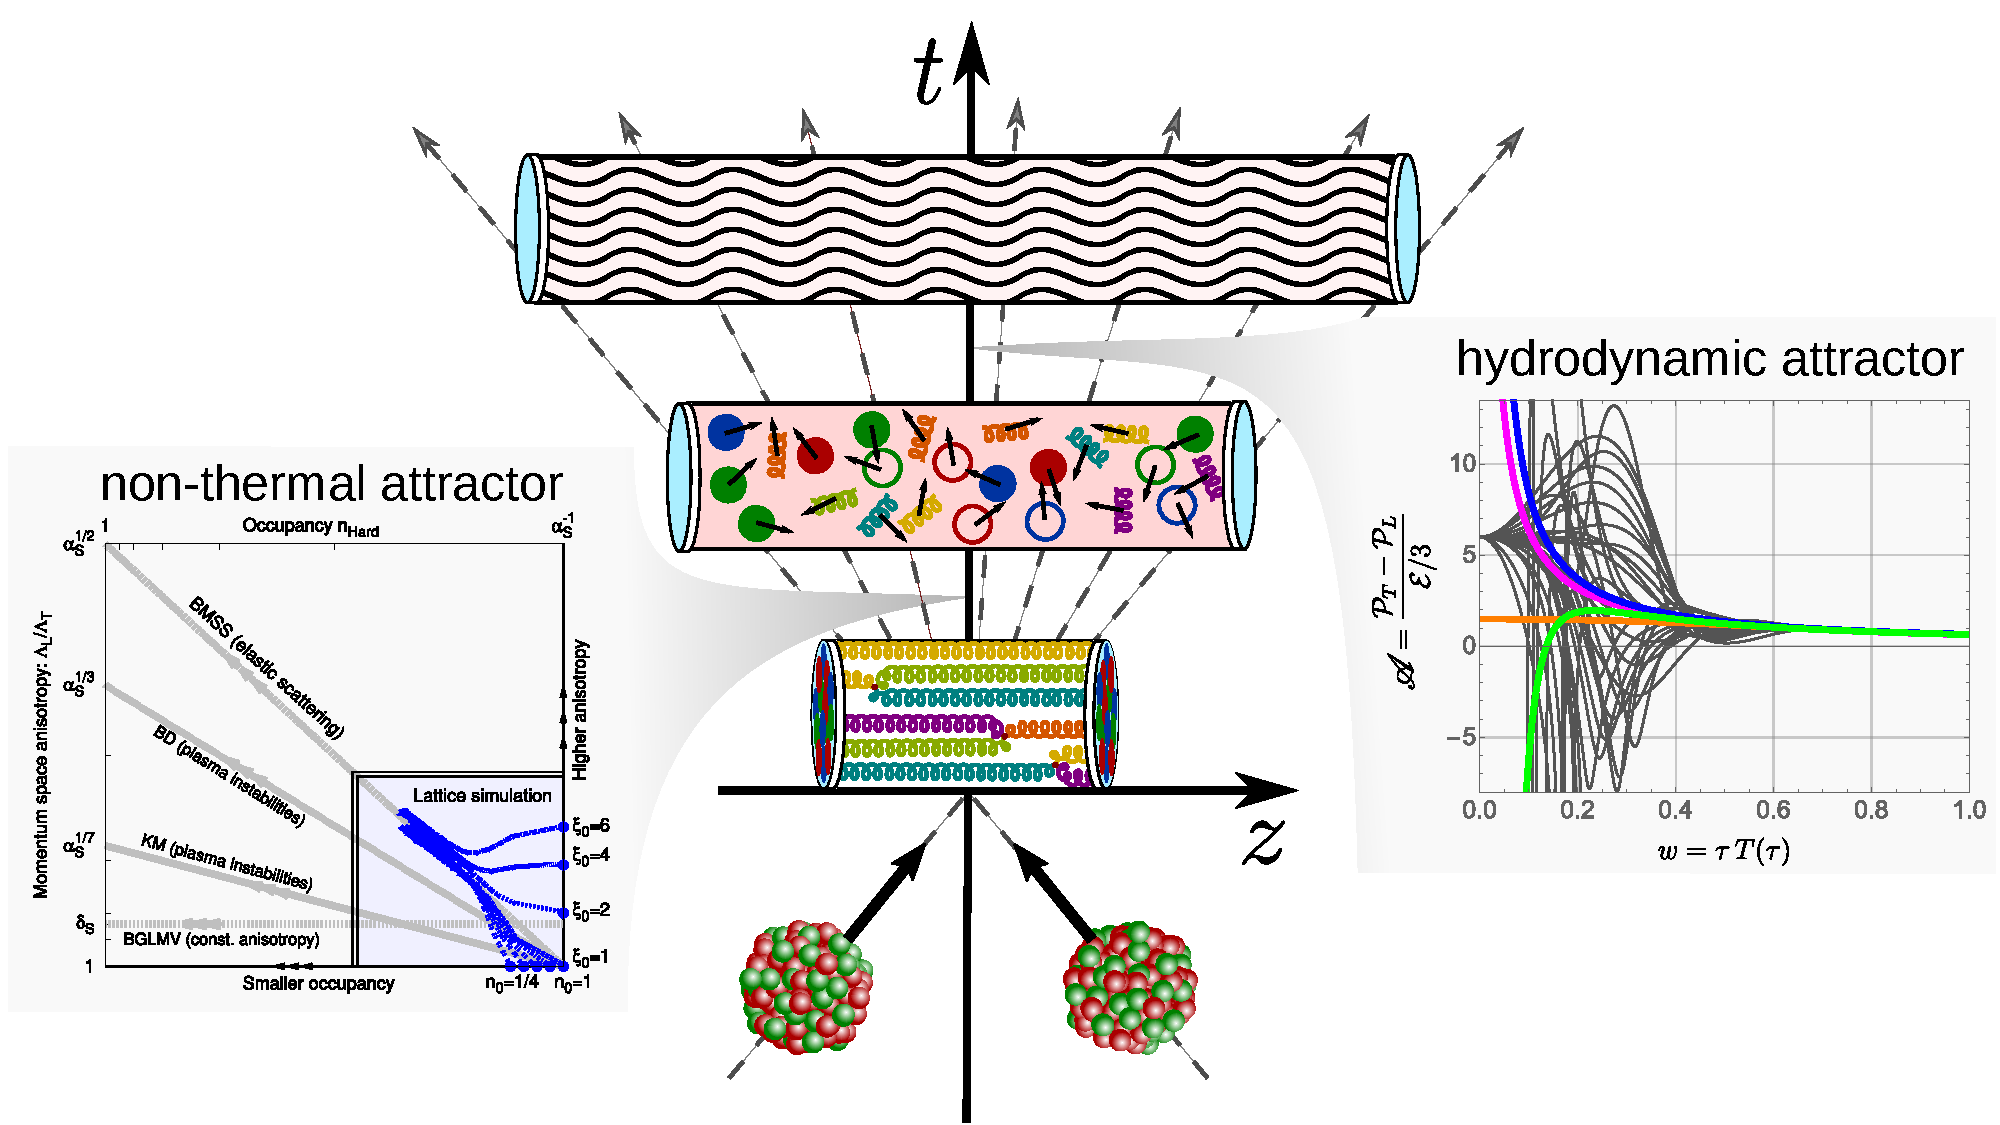
\includegraphics[height=0.7\paperheight]{images/fig01_cover_figure_RB10070_Berges.pdf}} \\[10pt]  
    {\transparent{0.2}\footnotesize\itshape Figure from  J. Berges, M. Heller, A. Mazeliauskas, R. Venugopalan \href{https://arxiv.org/abs/2005.12299}{{\color{lightgray}\texttt{[2005.12299]}}}}
   };
}
\begin{frame}{Brief outline}
    \begin{center}
        % \setlength{\leftskip}{\dimexpr.5\textwidth-.5\secnamelength\relax}% Advance left margin accordingly
        \tableofcontents
    \end{center}
\end{frame}
\setbeamertemplate{background}{}

\setbeamertemplate{background}{
\tikz[overlay,remember picture] \node[at=(current page.center), align=center] {
    \\[15pt]
    {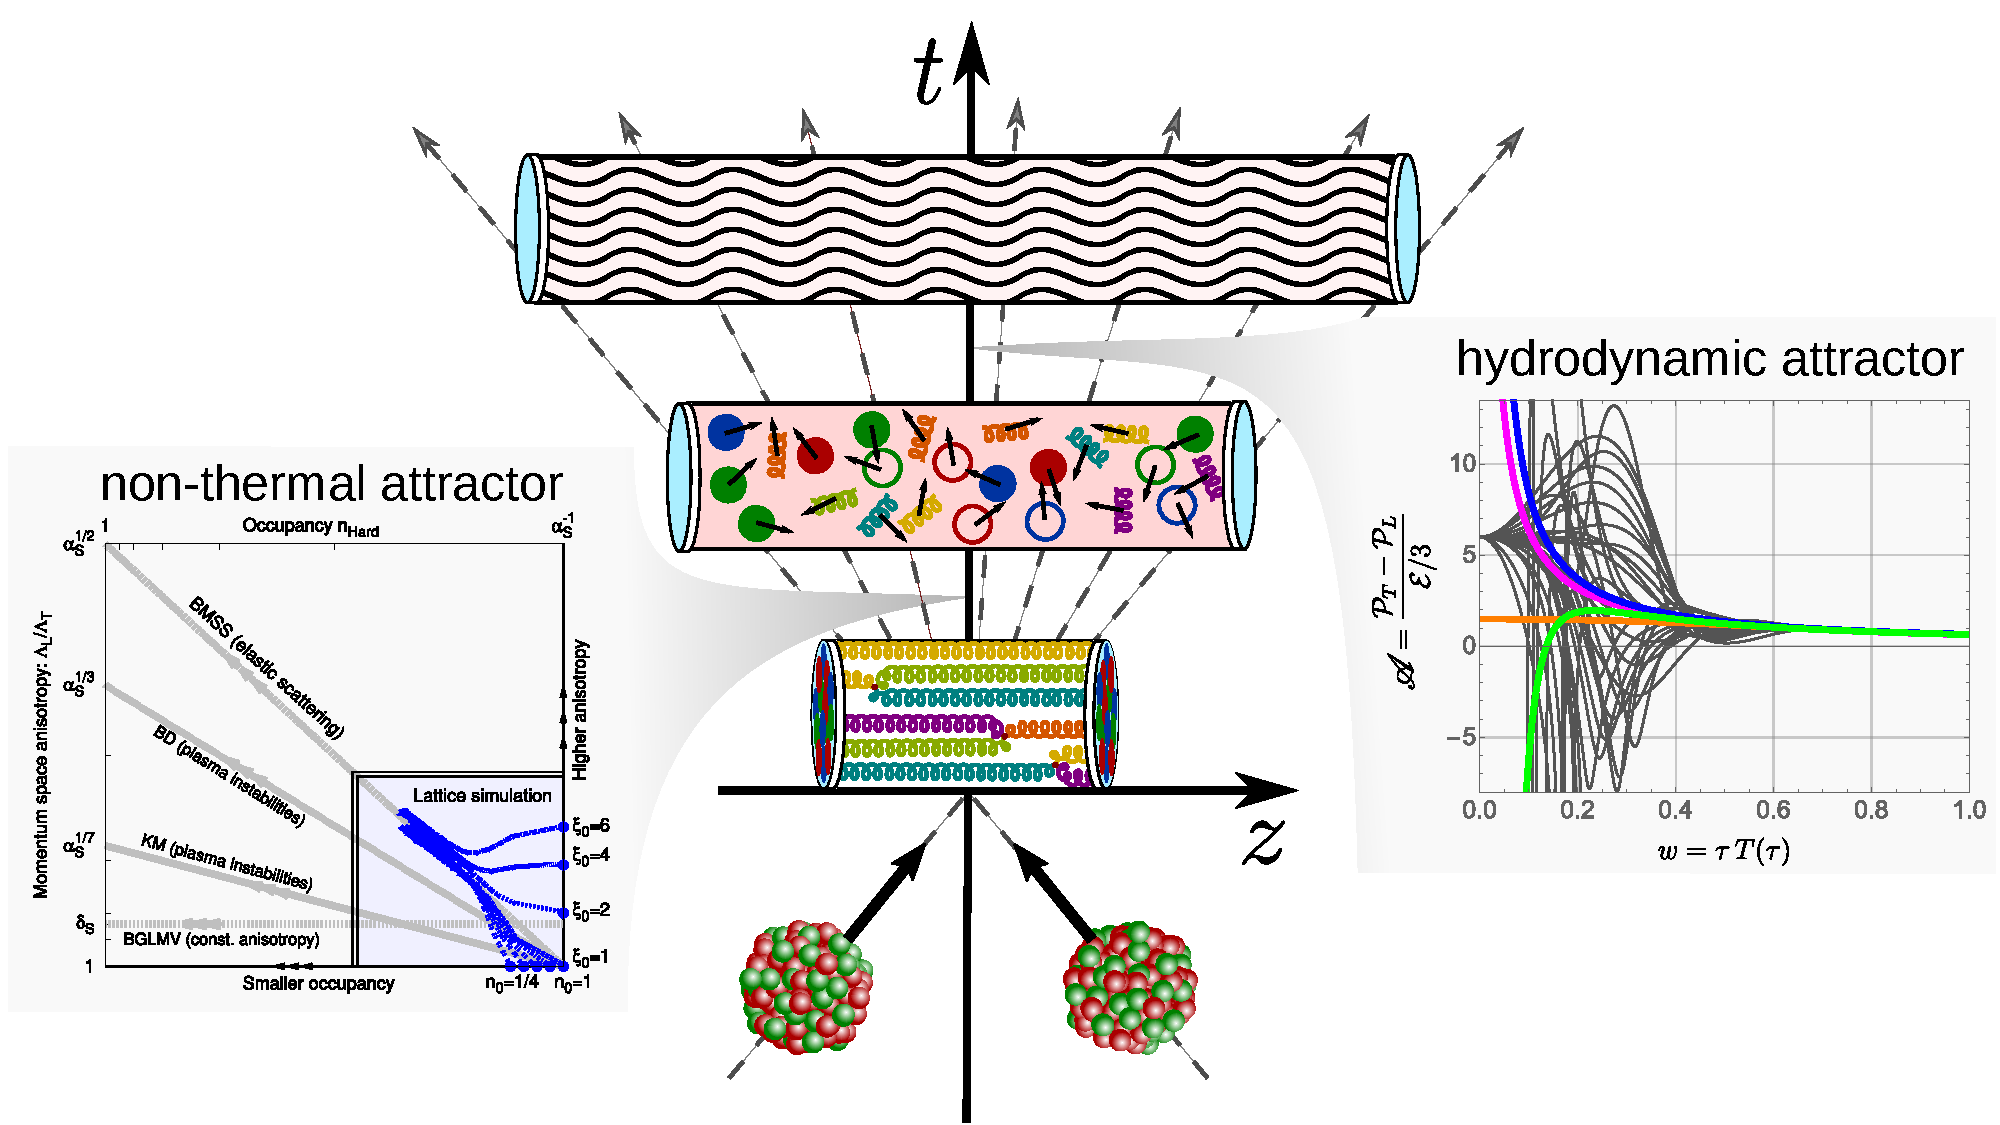
\includegraphics[height=0.7\paperheight]{images/fig01_cover_figure_RB10070_Berges.pdf}} \\[10pt]  
    {\footnotesize\itshape Figure from  J. Berges, M. Heller, A. Mazeliauskas, R. Venugopalan \href{https://arxiv.org/abs/2005.12299}{{\color{lightgray}\texttt{[2005.12299]}}}}
   };
}
\begin{frame}[noframenumbering]
    \frametitle{{\color{jyured}Pre-equilibrium} dynamics}
    % \begin{center}
    %     % \setlength{\leftskip}{\dimexpr.5\textwidth-.5\secnamelength\relax}% Advance left margin accordingly
    %     \tableofcontents
    % \end{center}
\end{frame}
\setbeamertemplate{background}{}


\setcounter{framenumber}{0}
\setbeamertemplate{footline}[progress bar]
\setbeamercolor{progress bar}{fg=customblue,bg=fondo}
\addtobeamertemplate{headline}{}{\vspace{1cm}\hfill\circcounter\hspace*{1cm}}
\addtobeamertemplate{frametitle}{\vspace{-0.8cm}}{}

%%%%%%%%%%%%%%%%%%%%%%%%%%%%%%%%%%%%%%%%%%%
%%%%%%%%%%%%%%%% SECTION 1 %%%%%%%%%%%%%%%%
%%%%%%%%%%%%%%%%%%%%%%%%%%%%%%%%%%%%%%%%%%%

\section{General context}

%%%%%%%%%%%%%%%%%%%%%%%%%%%%%%%%%%%%%%%%%%%
%%%%%%%%%%%%%%%%% SLIDE 1 %%%%%%%%%%%%%%%%%
%%%%%%%%%%%%%%%%%%%%%%%%%%%%%%%%%%%%%%%%%%%

\begin{frame}
    \frametitle{High-energy collisions}
    \framesubtitle{Stitching together effective theories}

    \begin{center}
        \begin{tikzpicture}
            \node[anchor=south west,inner sep=0] at (0,0) {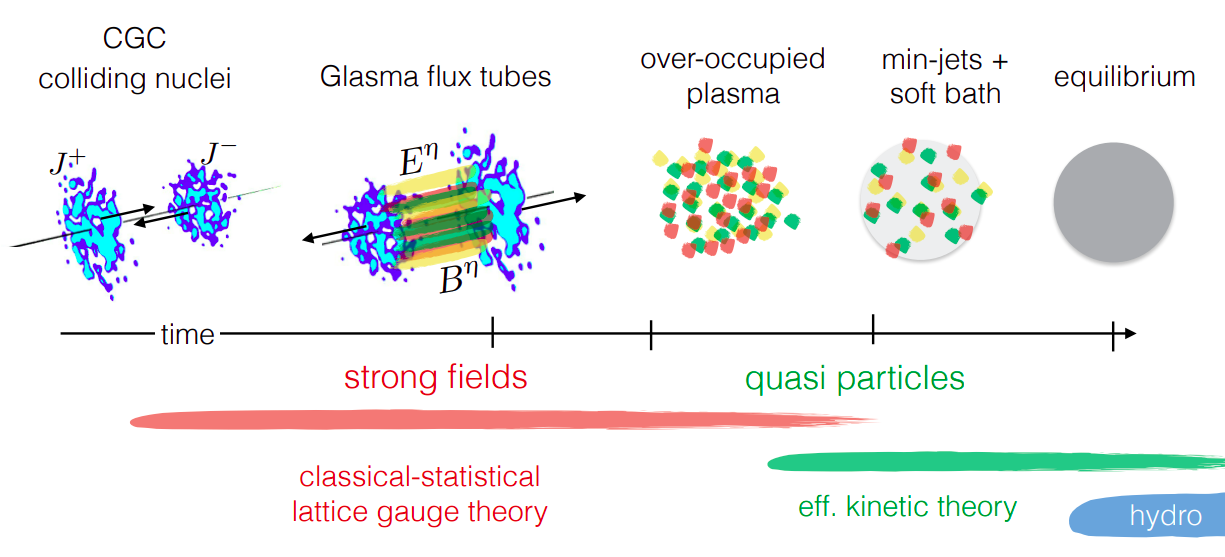
\includegraphics[width=0.8\textwidth]{images/schlichting_initial_stages_2016.png}};
            % \draw<1>[red,ultra thick,rounded corners] (1.6,1) rectangle (\textheight-1cm,5);
            % \draw<2>[red,ultra thick,rounded corners] (5.7,4.1) rectangle (7.5,4.9);
        \end{tikzpicture}
    \end{center}
        
    \begin{center}
        {\scriptsize\itshape Figure credits to S. Schlichting}
    \end{center}
\end{frame}

\setbeamertemplate{itemize item}{\raisebox{0.2em}{\scalebox{0.7}{${\color{pinky}\blacktriangleright}$}}} 

\begin{frame}[noframenumbering]
    \frametitle{High-energy collisions}
    \framesubtitle{{\color{jyured}Pre-equilibrium} stages}
    
    \begin{center}
        \begin{tikzpicture}[]
            \node[anchor=south west,inner sep=0] at (0,0) {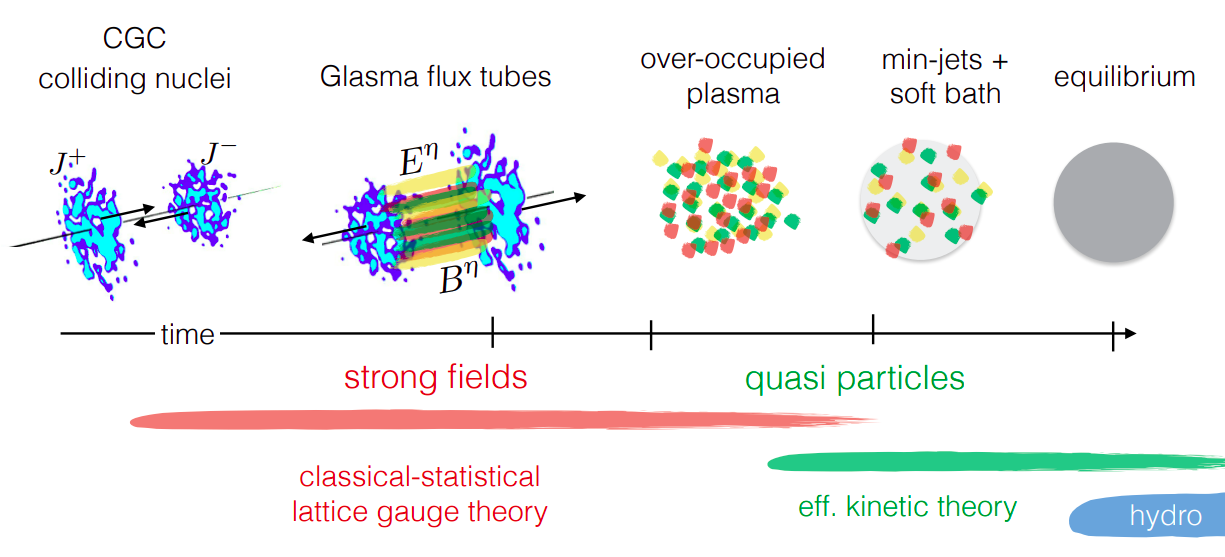
\includegraphics[width=0.8\textwidth]{images/schlichting_initial_stages_2016.png}};
            \draw<1>[white, fill=white, fill opacity=0.9] (8.37,0) rectangle (\textheight+4.6cm,5.5) node[pos=0.5, anchor=center, xshift=0.03\linewidth,text width=4cm] {{\Large\color{pinky} Glasma stage}\\[10pt]\footnotesize\begin{itemize}
                \item Gluons as color fields
                \item Classical gauge fields
                \item Weak coupling regime
                \item Color Glass Condensate
                \item Real-time classical lattice gauge theory
            \end{itemize}
            {\footnotesize\color{red}Add references}
            };
            \draw<1>[pinky,thick,fill=pinky,fill opacity=0.1] (0,0) rectangle (\textheight+0.6cm,5.5);
            % \draw<2>[red,ultra thick,rounded corners] (5.7,4.1) rectangle (7.5,4.9);
        \end{tikzpicture}
    \end{center}
        
    \begin{center}
        {\scriptsize\itshape Figure credits to S. Schlichting}
    \end{center}
\end{frame}

\setbeamertemplate{itemize item}{\raisebox{0.2em}{\scalebox{0.7}{${\color{ming}\blacktriangleright}$}}} 

\begin{frame}[noframenumbering]
    \frametitle{High-energy collisions}
    \framesubtitle{{\color{jyured}Pre-equilibrium} stages}
    
    \begin{center}
        \begin{tikzpicture}[]
            \node[anchor=south west,inner sep=0] at (0,0) {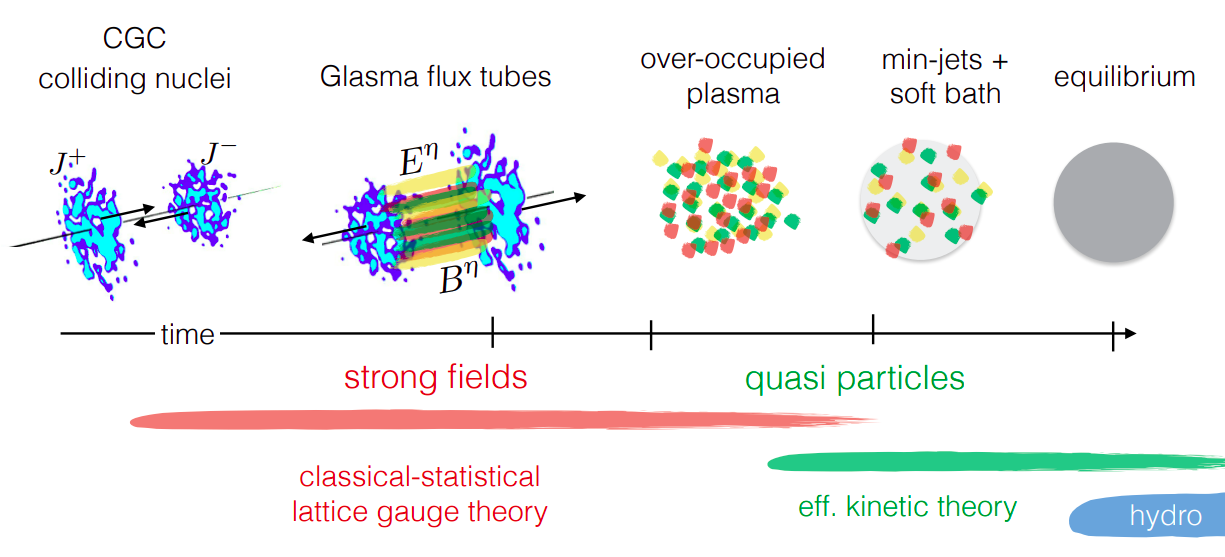
\includegraphics[width=0.8\textwidth]{images/schlichting_initial_stages_2016.png}};
            \draw<1>[white, fill=white, fill opacity=0.9] (0,0) rectangle (\textheight-1.55cm,5.5) node[pos=0.5, anchor=center, xshift=-0.01\linewidth,text width=5.5cm] {{\Large\color{ming} Kinetic theory}\\[10pt]\footnotesize\begin{itemize}
                \item Gluons as quasi-particles
                \item Distribution functions
                \item Weak coupling regime
                \item Bottom-up thermalization 
                \item AMY effective kinetic theory 
            \end{itemize}
            {\footnotesize\color{red}Add references}
            };
            \draw<1>[ming,thick,fill=ming,fill opacity=0.1] (6.2,0) rectangle (\textheight+4.6cm,5.5);
        \end{tikzpicture}
    \end{center}
        
    \begin{center}
        {\scriptsize\itshape Figure credits to S. Schlichting}
    \end{center}
\end{frame}

%%%%%%%%%%%%%%%%%%%%%%%%%%%%%%%%%%%%%%%%%%%
%%%%%%%%%%%%%%%% SECTION 2 %%%%%%%%%%%%%%%%
%%%%%%%%%%%%%%%%%%%%%%%%%%%%%%%%%%%%%%%%%%%

\section{{\color{jyured}Pre-equilibrium} dynamics}

\setbeamertemplate{background}{
\tikz[overlay,remember picture] \node[opacity=0.1, at=(current page.center), align=center] {
    \\[15pt]
    {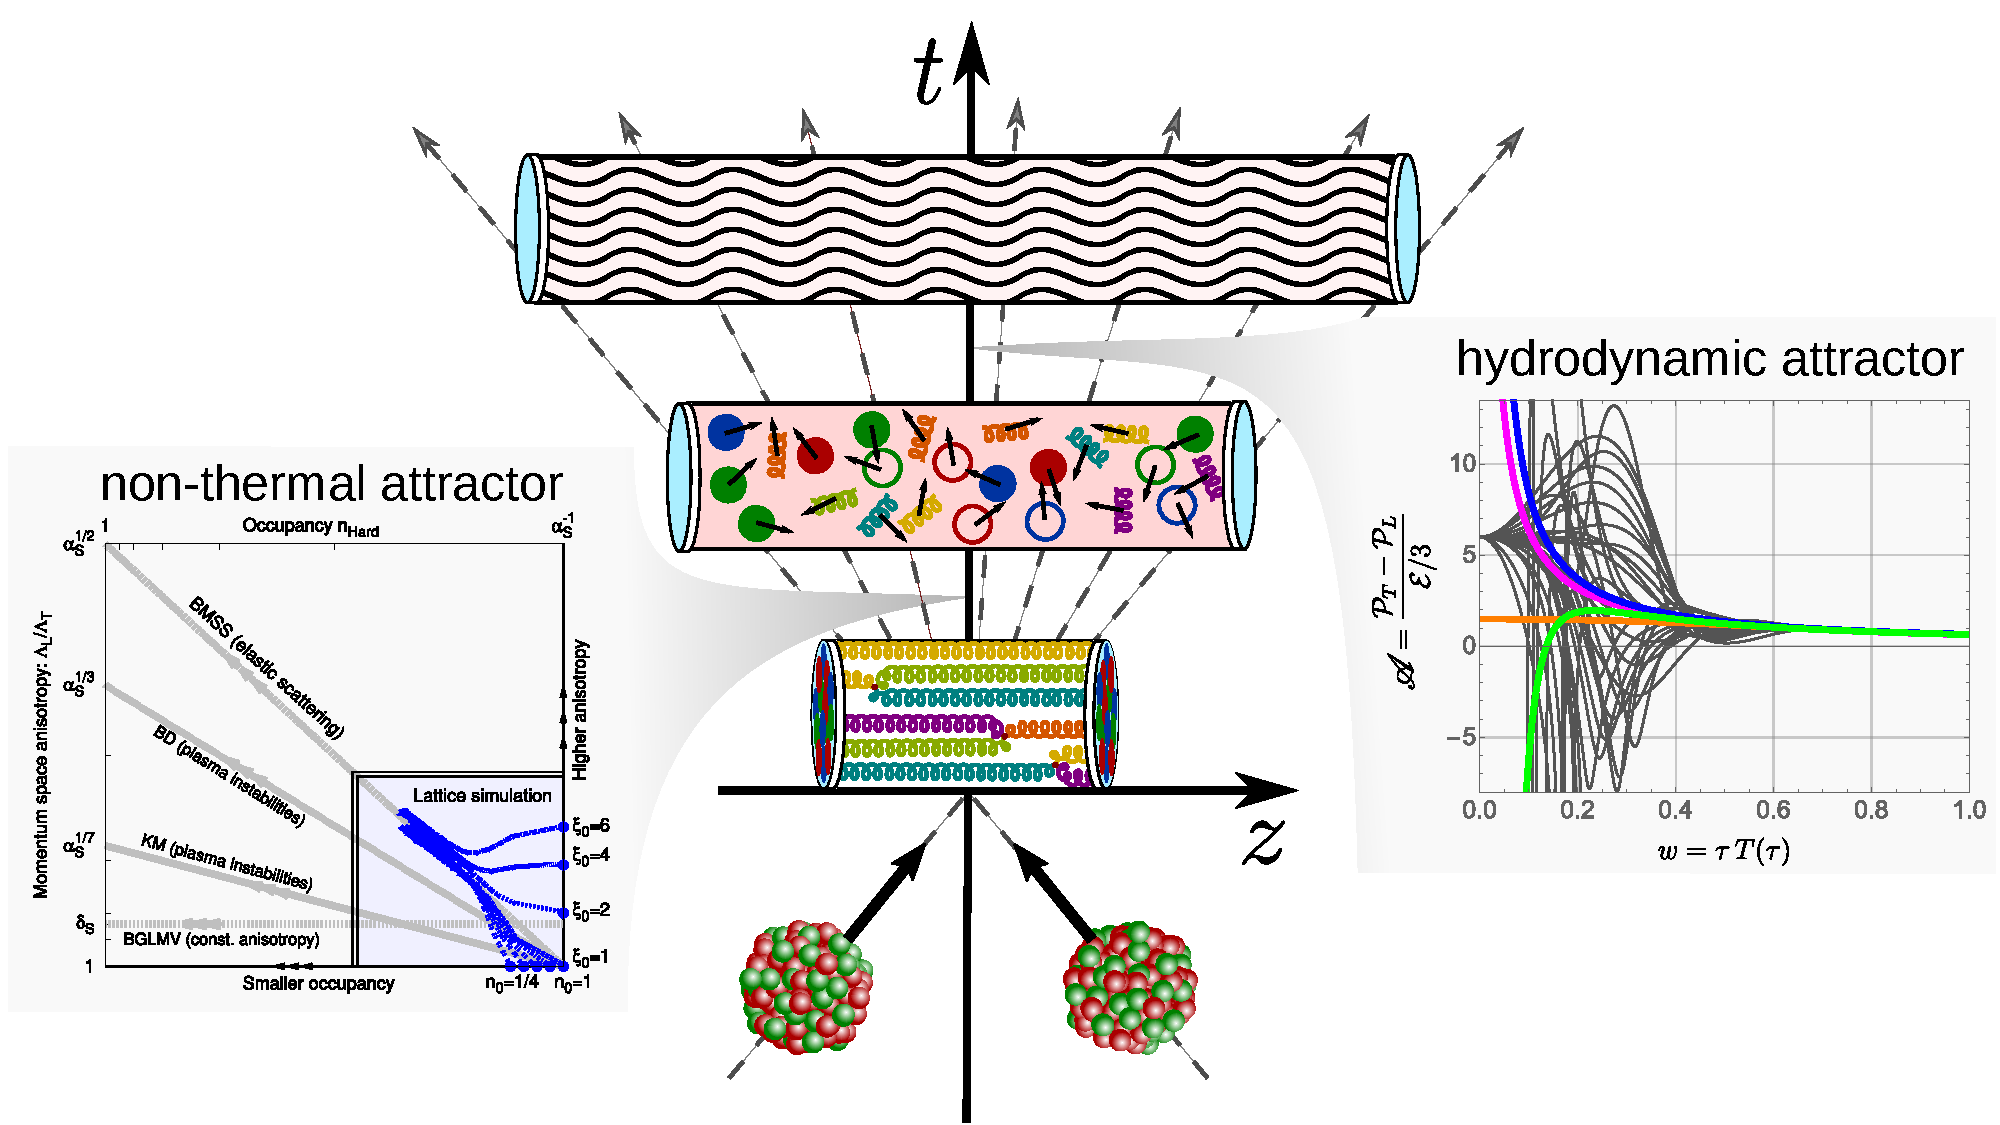
\includegraphics[height=0.7\paperheight]{images/fig01_cover_figure_RB10070_Berges.pdf}} \\[10pt]  
    {\footnotesize\itshape Figure from  J. Berges, M. Heller, A. Mazeliauskas, R. Venugopalan \href{https://arxiv.org/abs/2005.12299}{{\color{lightgray}\texttt{[2005.12299]}}}}
   };
}
\begin{frame}[plain, noframenumbering]
    \frametitle{\\{\color{jyured}Pre-equilibrium} dynamics}
    % \begin{center}
    %     {\Huge {\color{jyured}Pre-equilibrium} dynamics}
    % \end{center}
    % \\[20pt]
    \begin{center}
        % \huge {\color{jyured}Pre-equilibrium} frameworks \\
        {\huge {\color{pinky} Glasma} and {\color{ming}kinetic theory}}\\[20pt]
        {\footnotesize\itshape Other frameworks for pre-equilibrium dynamics are not included in this talk\\
        {\color{red}Add references}}
    \end{center}
\end{frame}
\setbeamertemplate{background}{}

\subsection{Glasma}

\setbeamertemplate{background}{
\tikz[overlay,remember picture] \node[opacity=0.1, at=(current page.center), align=center] {\\[10pt]
{\transparent{0.2}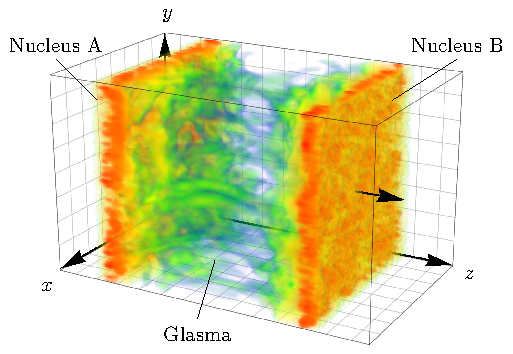
\includegraphics[height=0.8\paperheight]{images/fig1_overview.pdf}}
   \\[10pt]  
   {\transparent{0.5}\footnotesize\itshape Figure from  A. Ipp, D. Müller \href{https://arxiv.org/abs/1703.00017}{{\color{lightgray}\texttt{[1703.00017]}}}}};
}
\begin{frame}[plain,noframenumbering]{}
    \begin{center}
        \vspace{1cm}
        {\large\color{normal}Initial stage of pre-equilibrium}\\[0.3cm]
        {\huge\color{destacado}The glasma}
    \end{center}
\end{frame}
\setbeamertemplate{background}{}

\begin{frame}
    \frametitle{Color Glass Condensate}
    \framesubtitle{An EFT for high energy QCD}
    \vspace{-10pt}
    \begin{columns}[onlytextwidth,t]
        \column{.033\textwidth}
       \column{.5\textwidth}
            \begin{center}
                {\footnotesize Separation of scales between\\
                {\color{customgreen}small-{\tiny $x$}} and {\color{custompink}large-{\huge $x$}} degrees of freedom}
            \end{center}
            \vspace{-10pt}
            \begin{figure}[!hbt]
                \centering
                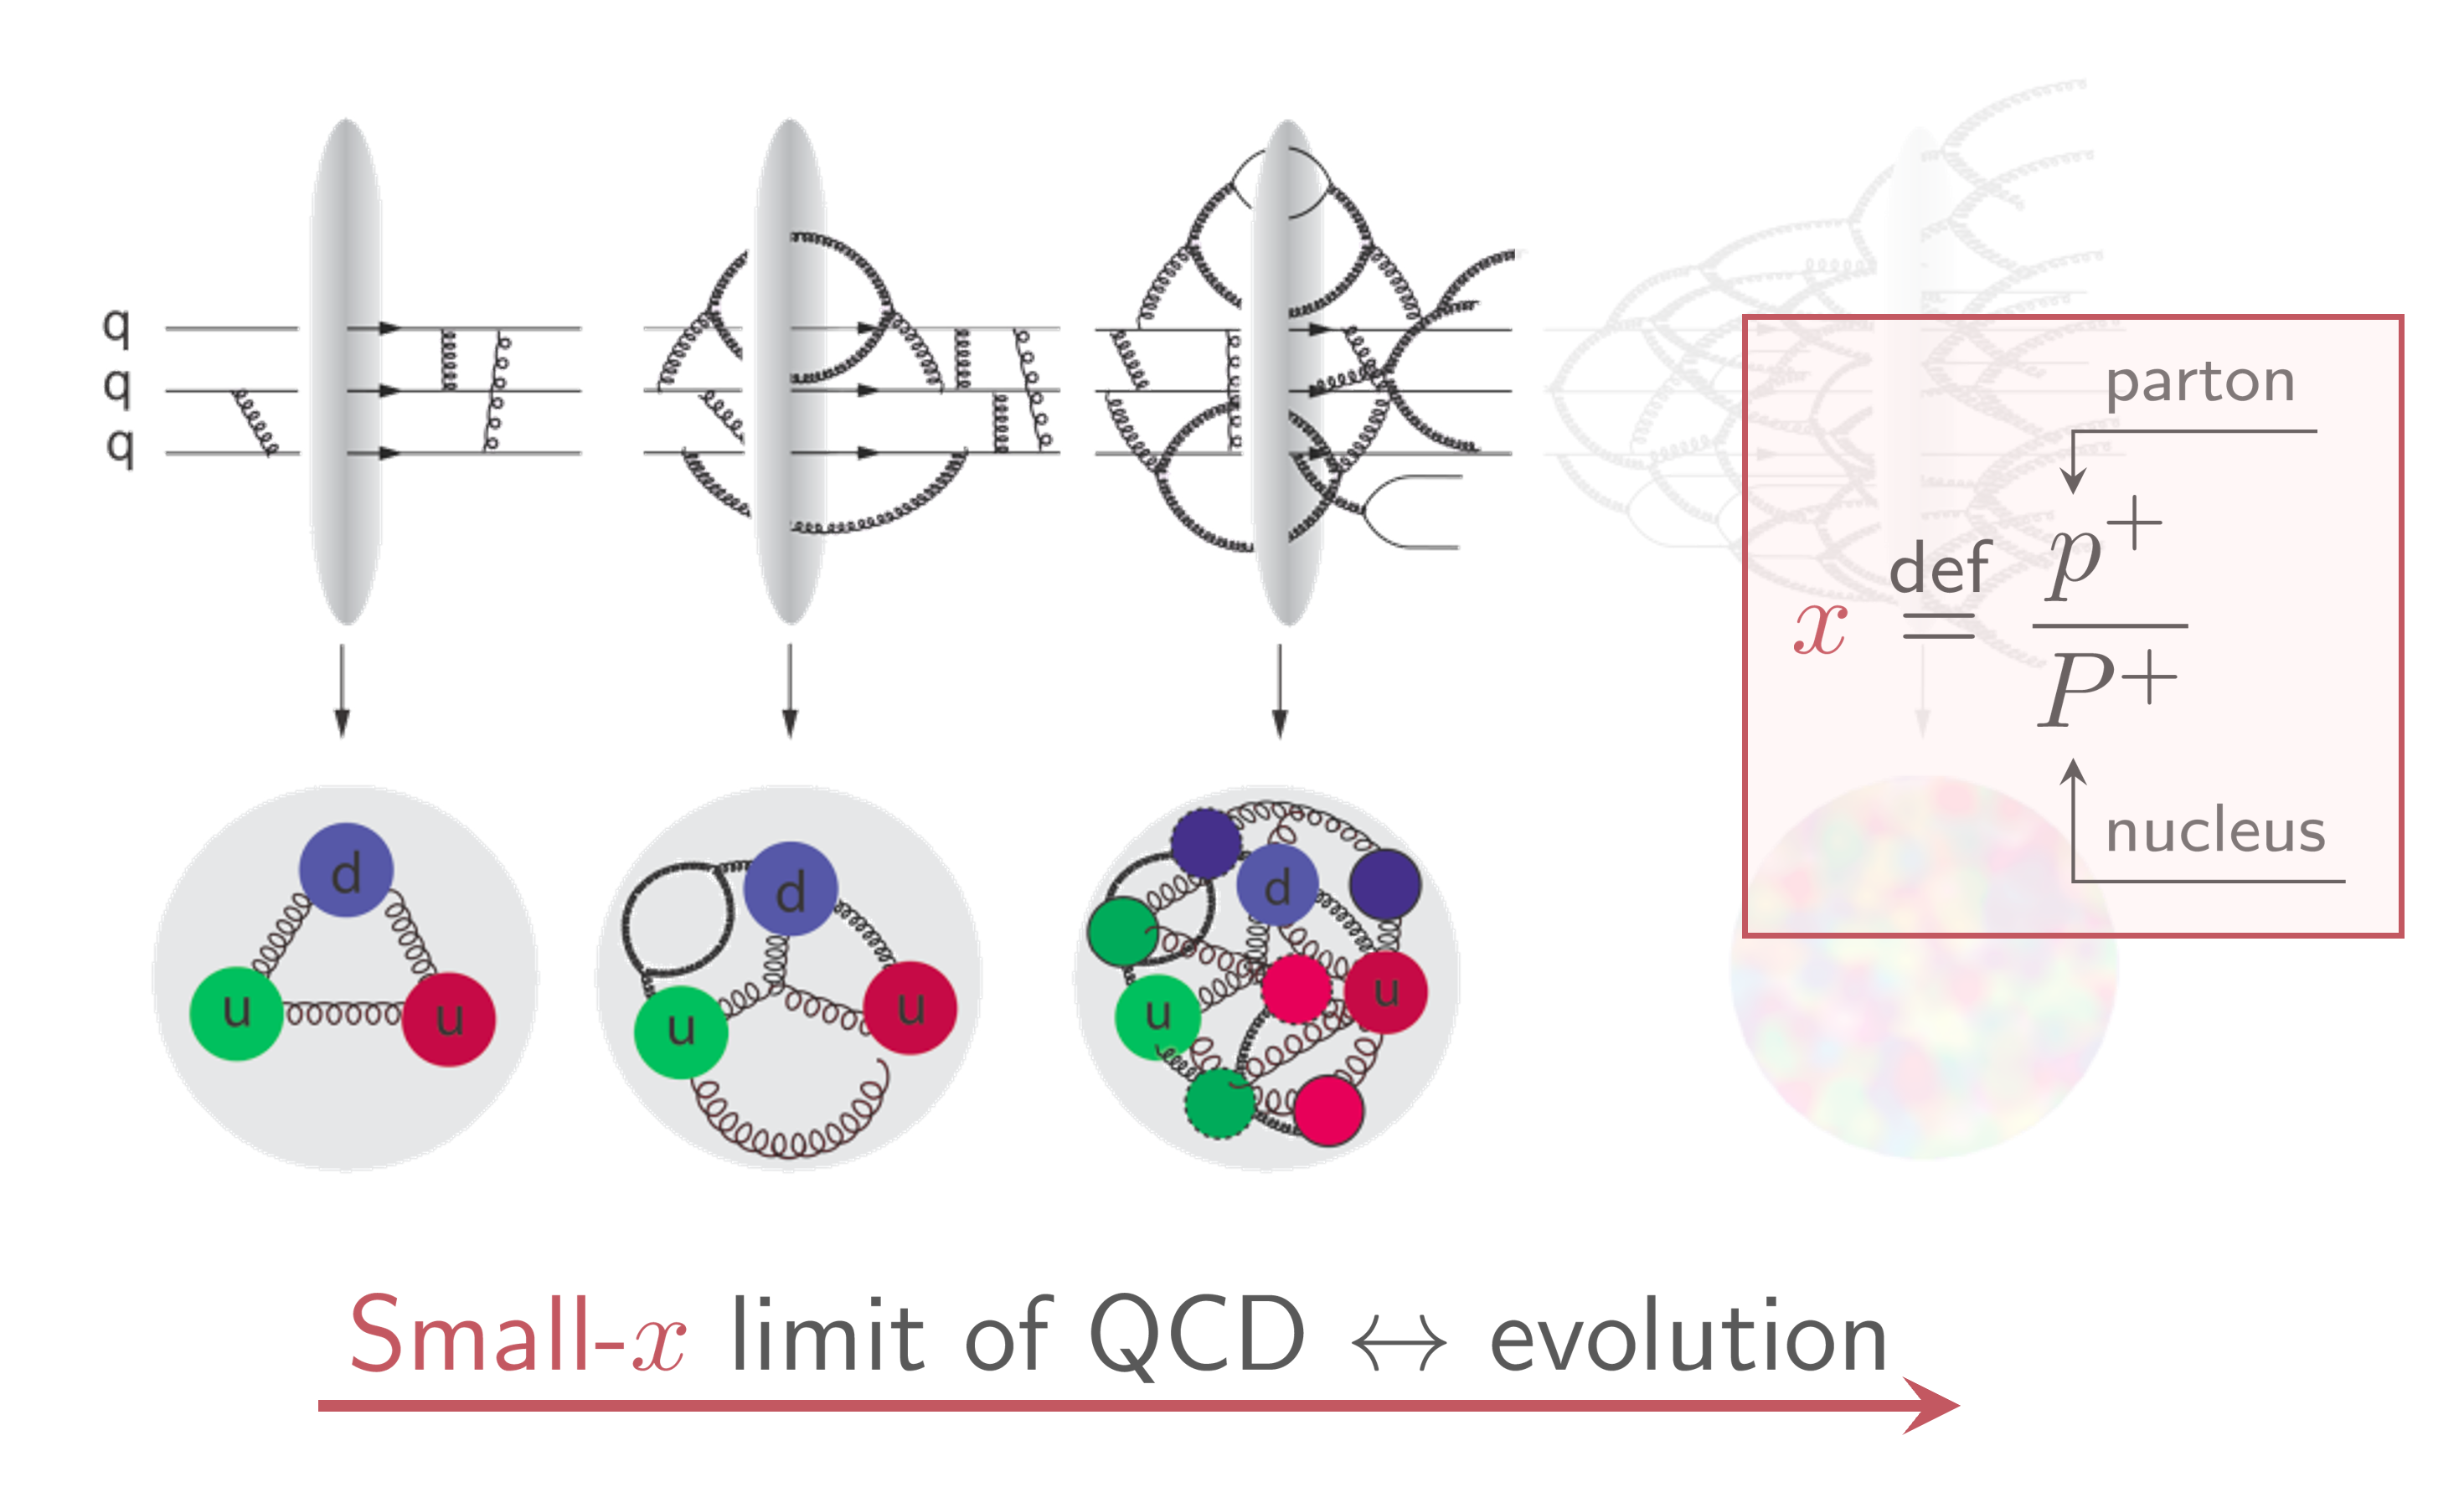
\includegraphics[width=\textwidth]{images/qcd_1.png}
                \captionsetup{justification=centering}
                \vspace{-20pt}
                \caption{\tiny\itshape Figure credits to T. Ullrich}
            \end{figure}
        \column{.033\textwidth}
        \column{.4\textwidth}
        \begin{center}
            {\transparent{0.2}
            \begin{figure}[!hbt]
                \centering
                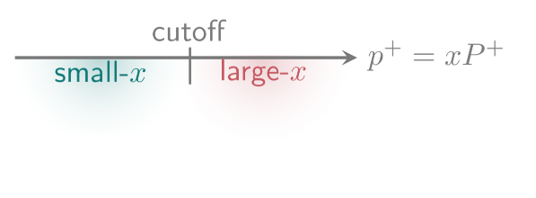
\includegraphics[width=0.9\textwidth]{images/small_large_x.png}
                \captionsetup{justification=centering}
                \vspace{-0.2em}
            \end{figure}
            \footnotesize
            \vspace{-10pt}
            Classical Yang-Mills equations\\[20pt]
            \renewcommand{\eqnhighlightheight}{\vphantom{\mathcal{D}_\mu}\mathstrut}\begin{equation*}
                \Big(\eqnmark[starrymain]{dmu}{\mathcal{D}_\mu}\eqnmark[starrysecond]{fmunu}{F^{\mu\nu}}\Big)\Big[\eqnmark[customgreen]{amu}{A^\mu}\Big]=\eqnmark[custompink]{jnu}{J^\nu}
                \end{equation*}
                \annotate[yshift=2.2em]{above, right}{dmu}{\scriptsize covariant derivative}
                \annotate[yshift=0.7em]{above}{fmunu}{\scriptsize field strength tensor}
                \annotate[yshift=-0.5em]{below, left}{amu}{\scriptsize gluons gauge field}
                \annotate[yshift=-2em]{below, left}{jnu}{\scriptsize color current of nucleus}}
        \end{center}
        \column{.033\textwidth}
    \end{columns}
\end{frame}

\begin{frame}[noframenumbering]
    \frametitle{Color Glass Condensate}
    \framesubtitle{An EFT for high energy QCD}
    \vspace{-10pt}
    \begin{columns}[onlytextwidth,t]
        \column{.033\textwidth}
       \column{.5\textwidth}
            \begin{center}
                {\footnotesize Separation of scales between\\
                {\color{customgreen}small-{\tiny $x$}} and {\color{custompink}large-{\huge $x$}} degrees of freedom}
            \end{center}
            \vspace{-10pt}
            \begin{figure}[!hbt]
                \centering
                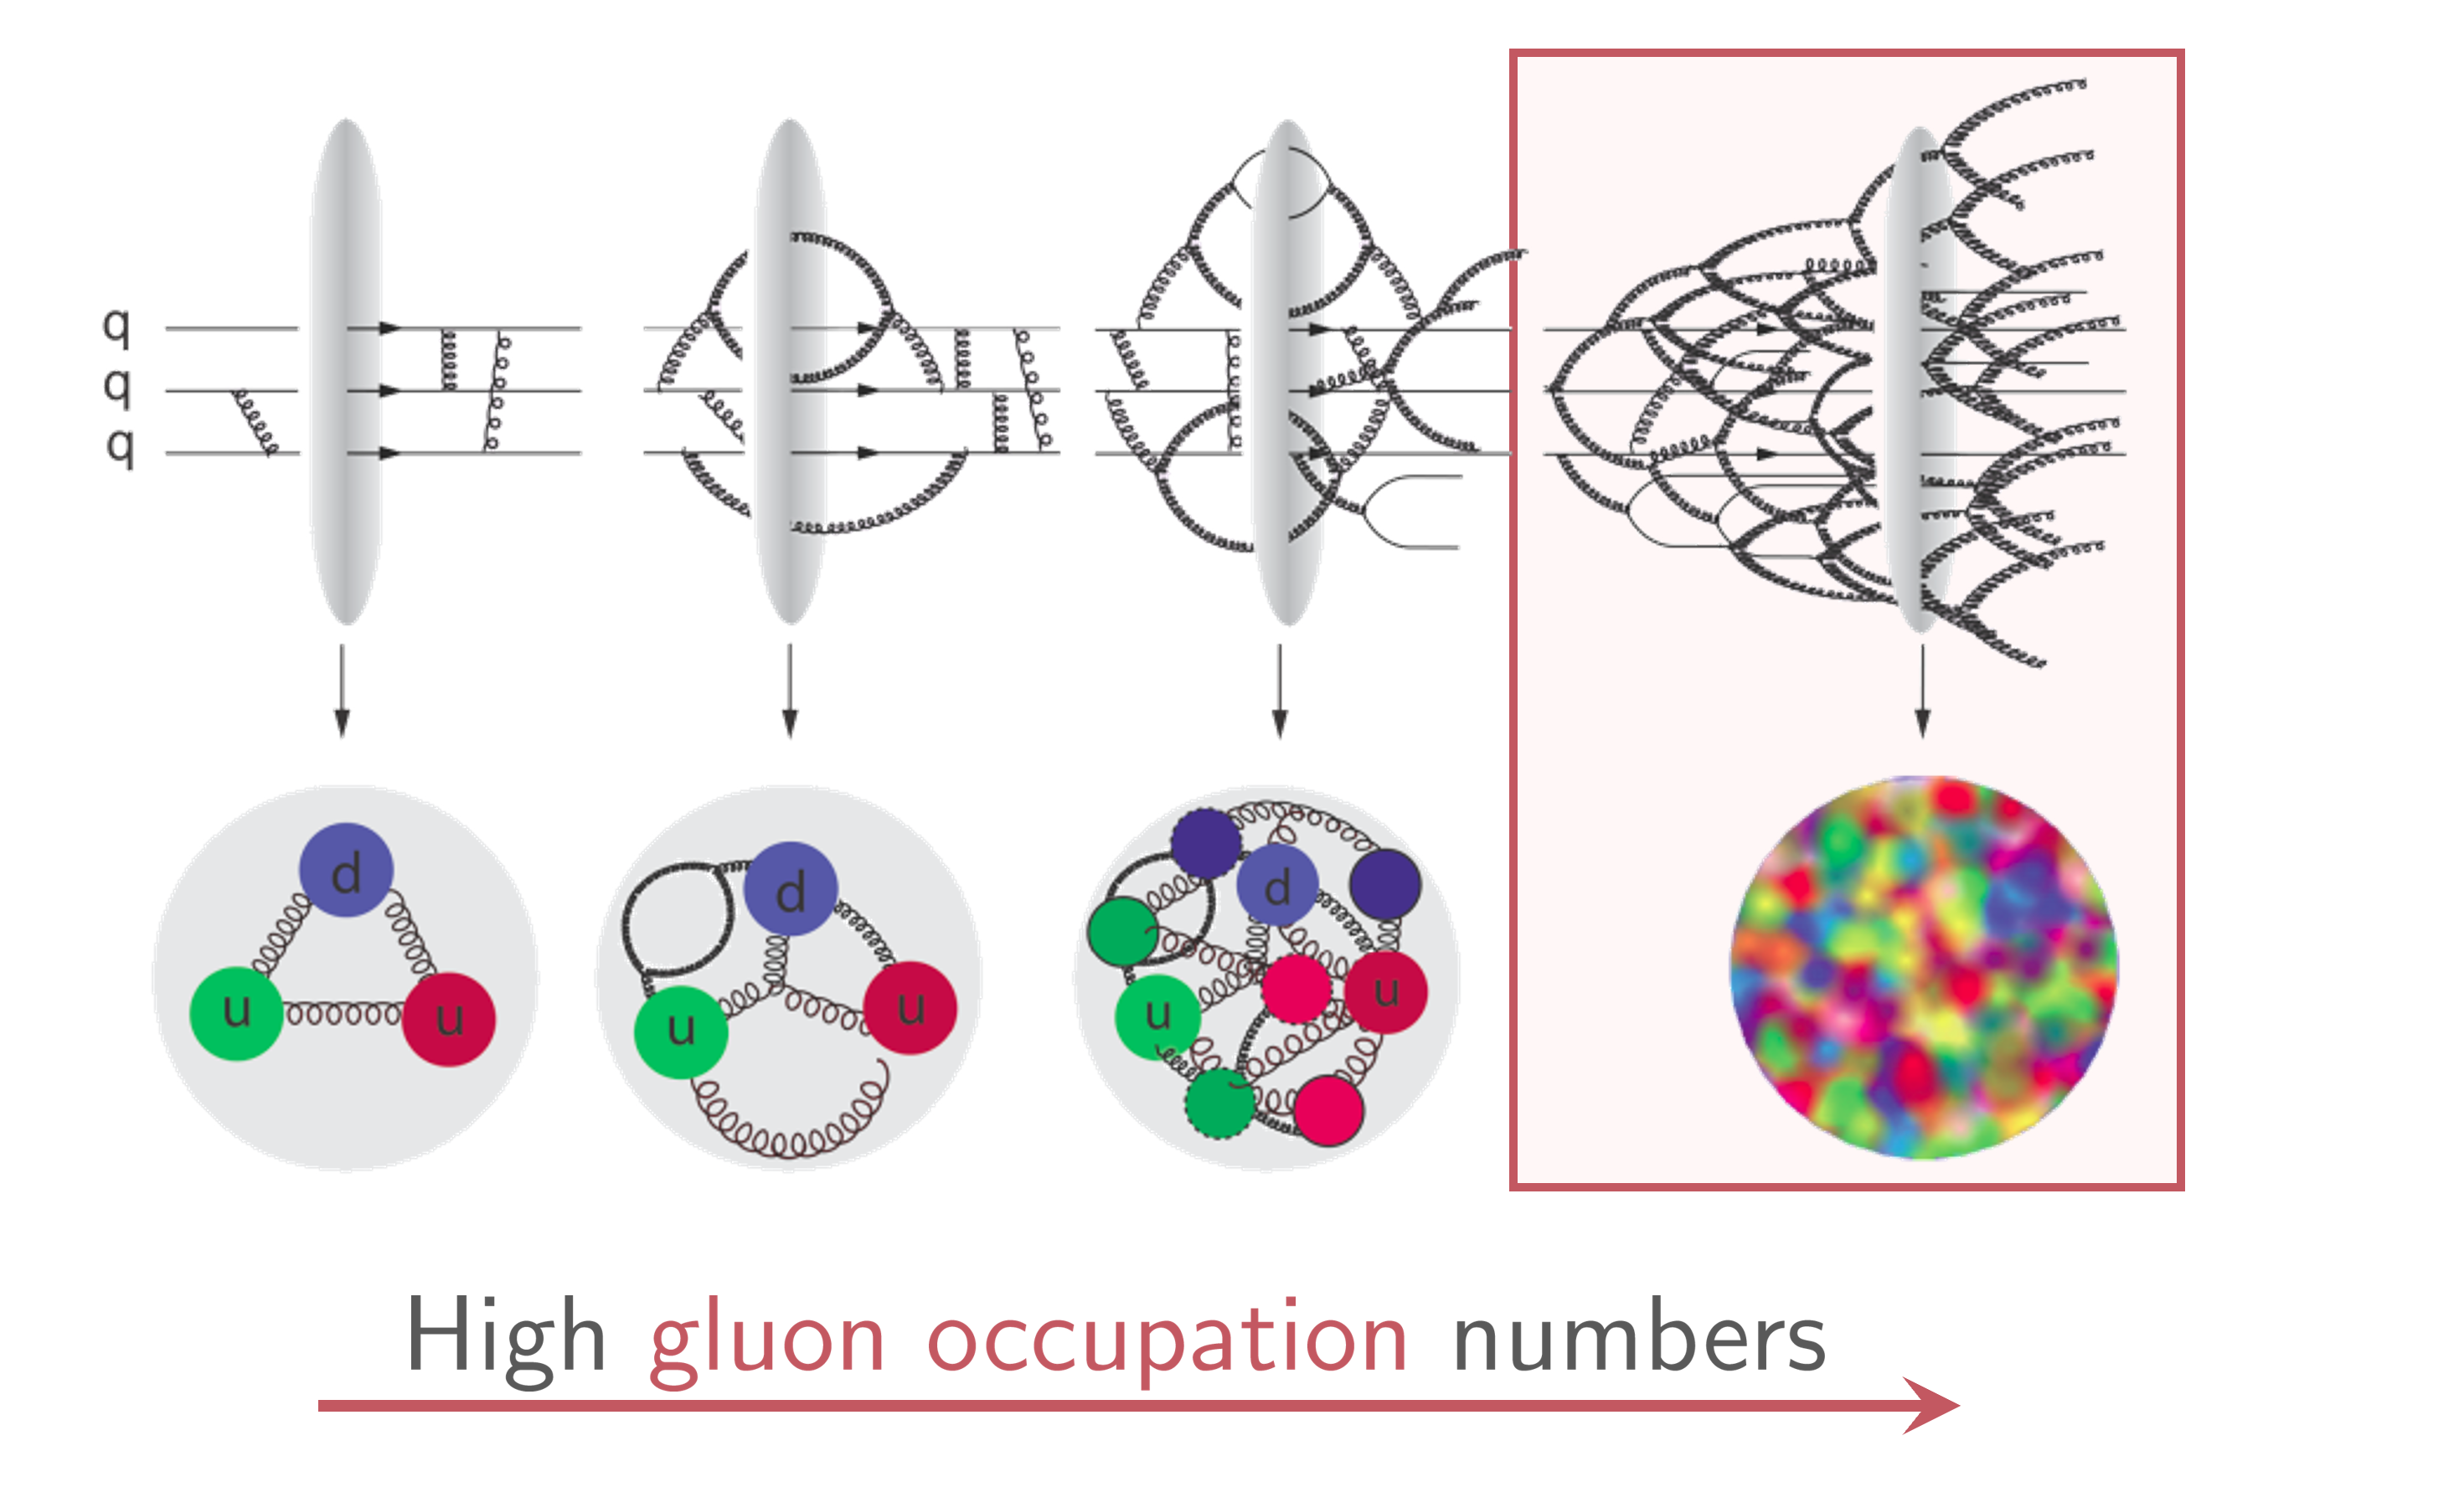
\includegraphics[width=\textwidth]{images/qcd_2.png}
                \captionsetup{justification=centering}
                \vspace{-20pt}
                \caption{\tiny\itshape Figure credits to T. Ullrich}
            \end{figure}
        \column{.033\textwidth}
        \column{.4\textwidth}
        \begin{center}
            \begin{figure}[!hbt]
                \centering
                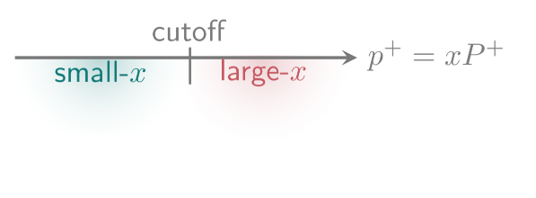
\includegraphics[width=0.9\textwidth]{images/small_large_x.png}
                \captionsetup{justification=centering}
                \vspace{-0.2em}
            \end{figure}
            \footnotesize
            \vspace{-10pt}
            Classical Yang-Mills equations\\[20pt]
            \renewcommand{\eqnhighlightheight}{\vphantom{\mathcal{D}_\mu}\mathstrut}\begin{equation*}
                \Big(\eqnmark[starrymain]{dmu}{\mathcal{D}_\mu}\eqnmark[starrysecond]{fmunu}{F^{\mu\nu}}\Big)\Big[\eqnmark[customgreen]{amu}{A^\mu}\Big]=\eqnmark[custompink]{jnu}{J^\nu}
                \end{equation*}
                \annotate[yshift=2.2em]{above, right}{dmu}{\scriptsize covariant derivative}
                \annotate[yshift=0.7em]{above}{fmunu}{\scriptsize field strength tensor}
                \annotate[yshift=-0.5em]{below, left}{amu}{\scriptsize gluons gauge field}
                \annotate[yshift=-2em]{below, left}{jnu}{\scriptsize color current of nucleus}
                {\footnotesize\color{red}Add references}
        \end{center}
        \column{.033\textwidth}
    \end{columns}
\end{frame}

\begin{frame}
    \frametitle{CGC fields}
    \framesubtitle{Analytical fields before the collision}
        % \begin{center}
        %     Initial stage using {\color{customblue}Color Glass Condensate} $\leftrightarrow$ EFT for high energy QCD \\
        %     High energy nucleus $\leadsto$ many gluons 
        %     % $\Leftrightarrow$ high occupation numbers for gluon fields \\ 
        %     $\Rightarrow$ classical colored fields $\equiv$ {\color{custompink}Glasma}
        % \end{center}
    % \vspace{-0.2cm}
    \begin{figure}[!hbt]
        \centering
    	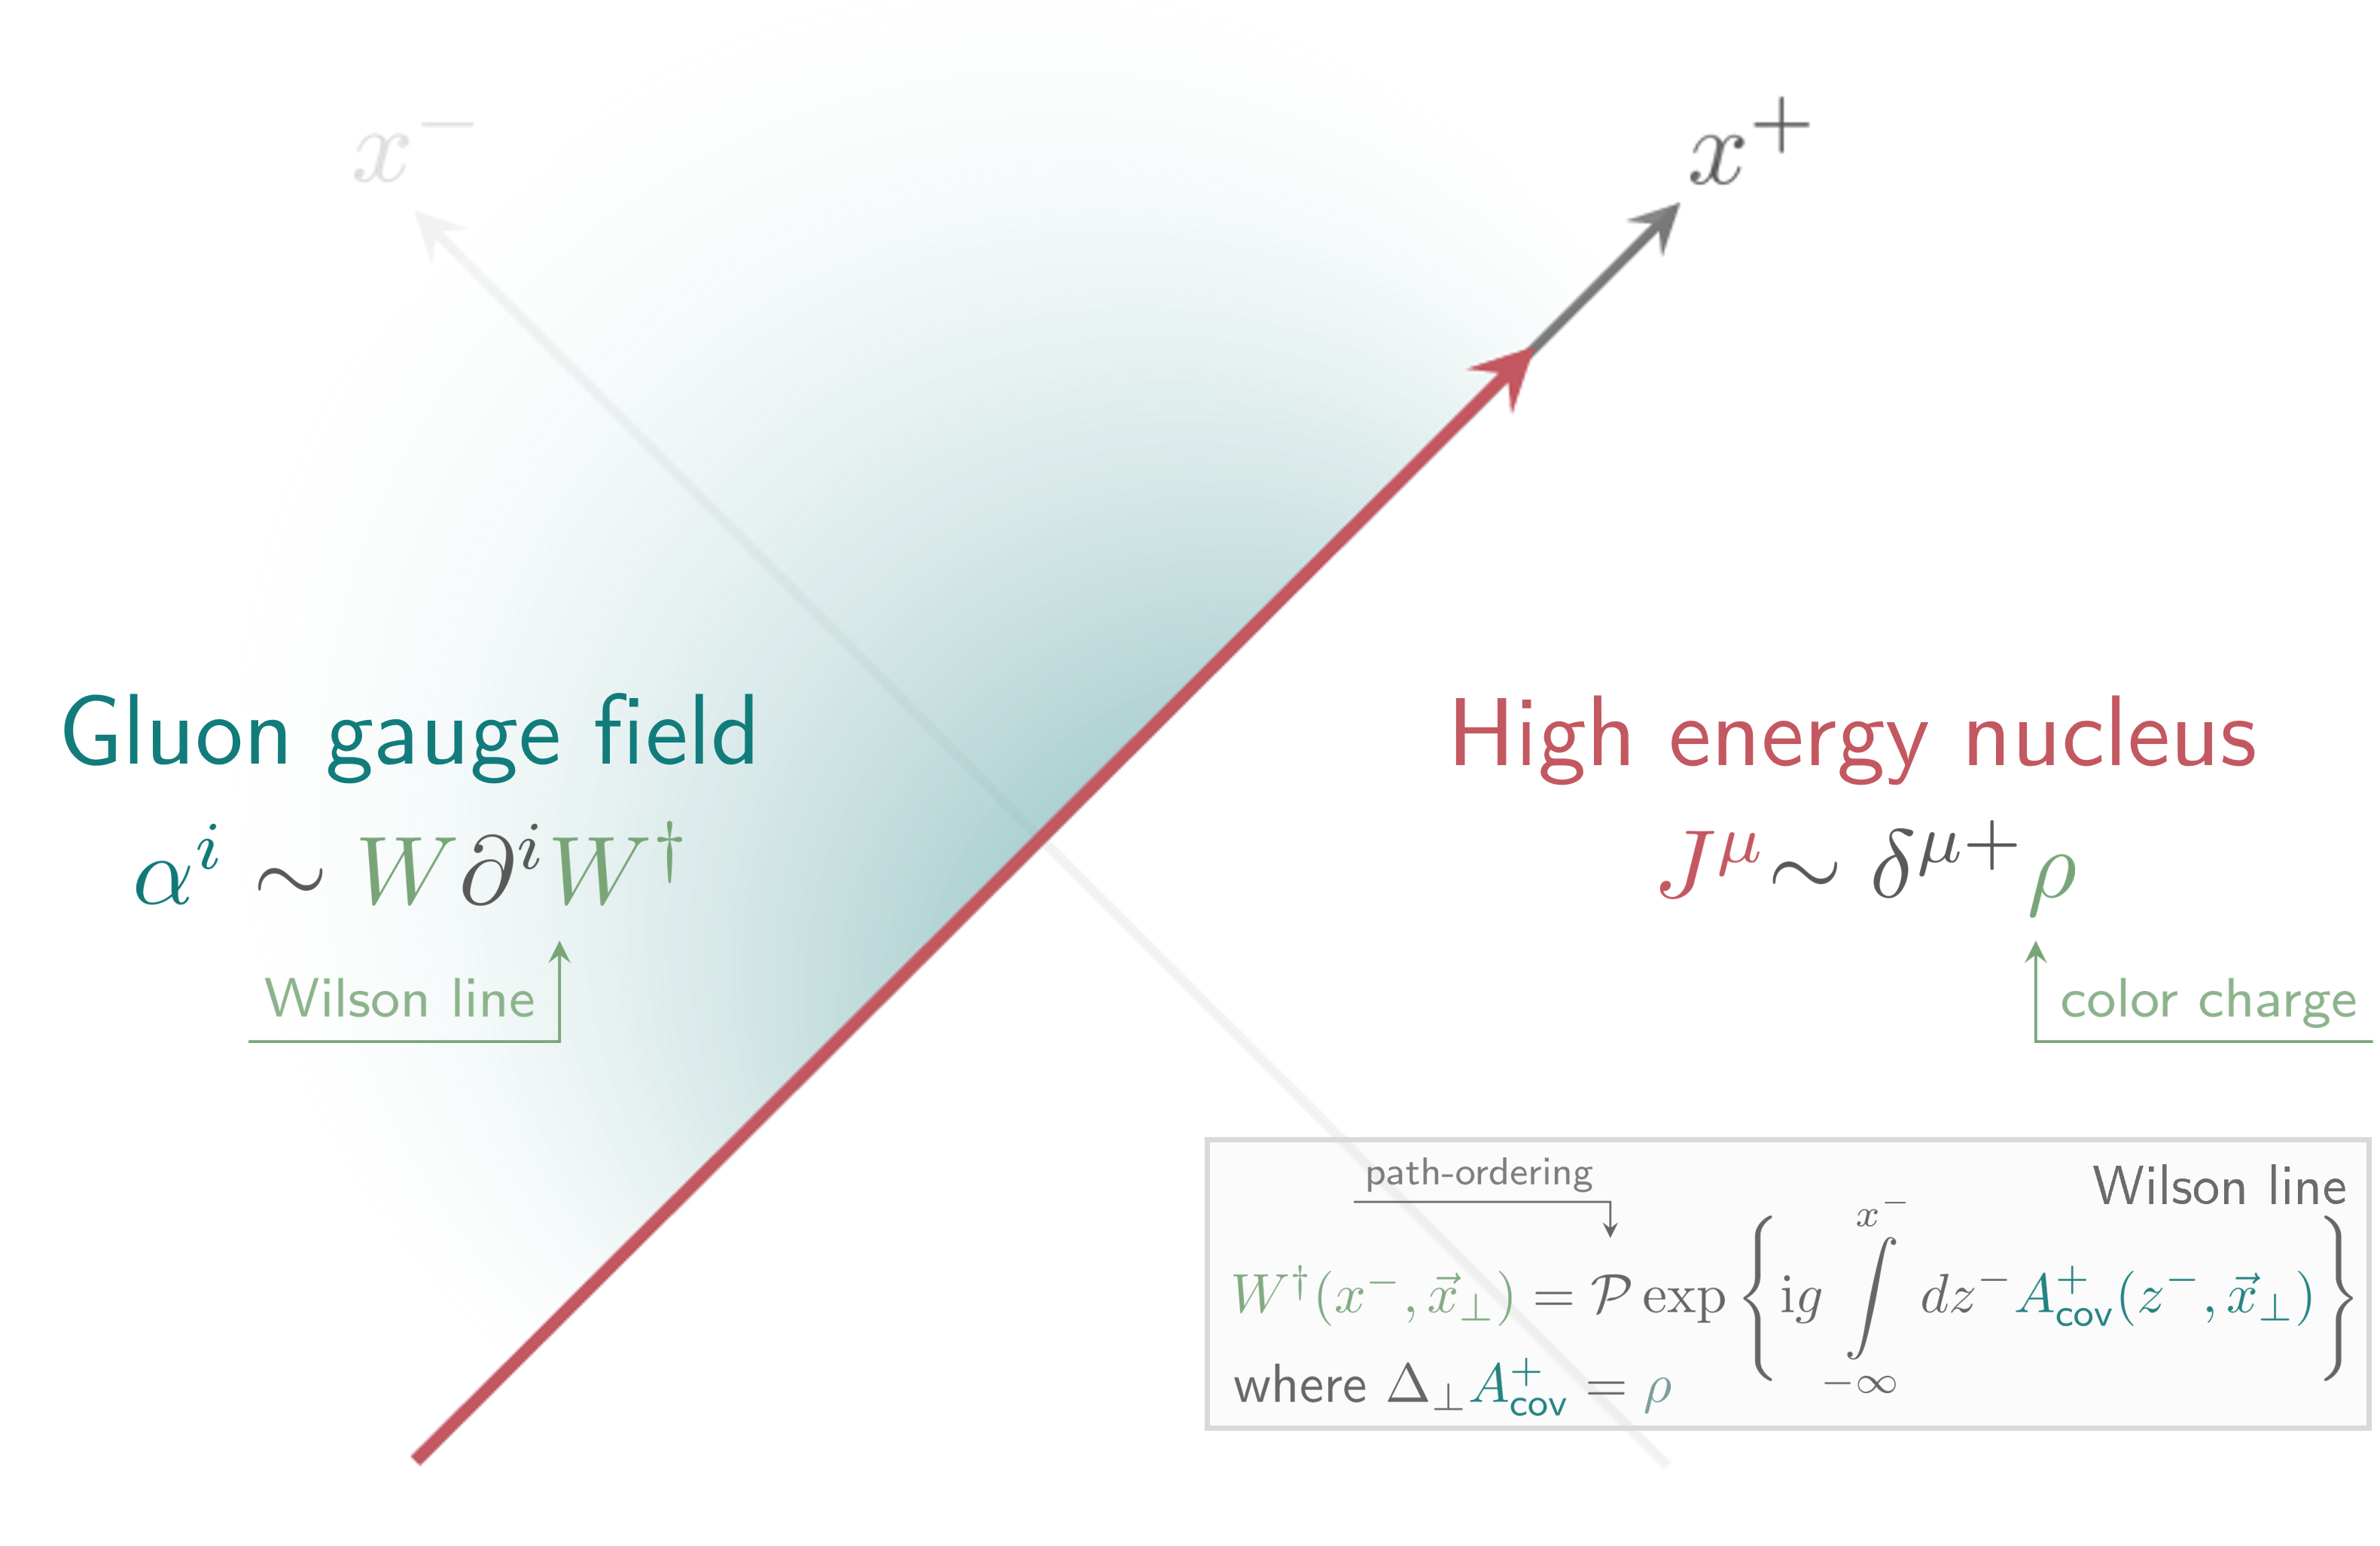
\includegraphics[width=0.7\textwidth]{images/cgc_nuclei.png}
        \captionsetup{justification=centering}
    \end{figure}
    {\footnotesize\color{red}Add references}
\end{frame}


% \addtocounter{framenumber}{-1}
\begin{frame}[noframenumbering]
    \frametitle{Glasma fields}
    \framesubtitle{Numerical field after the collision}
    \begin{columns}[onlytextwidth,t]
        \column{.02\textwidth}
       \column{.46\textwidth}
       \begin{figure}
            \centering
            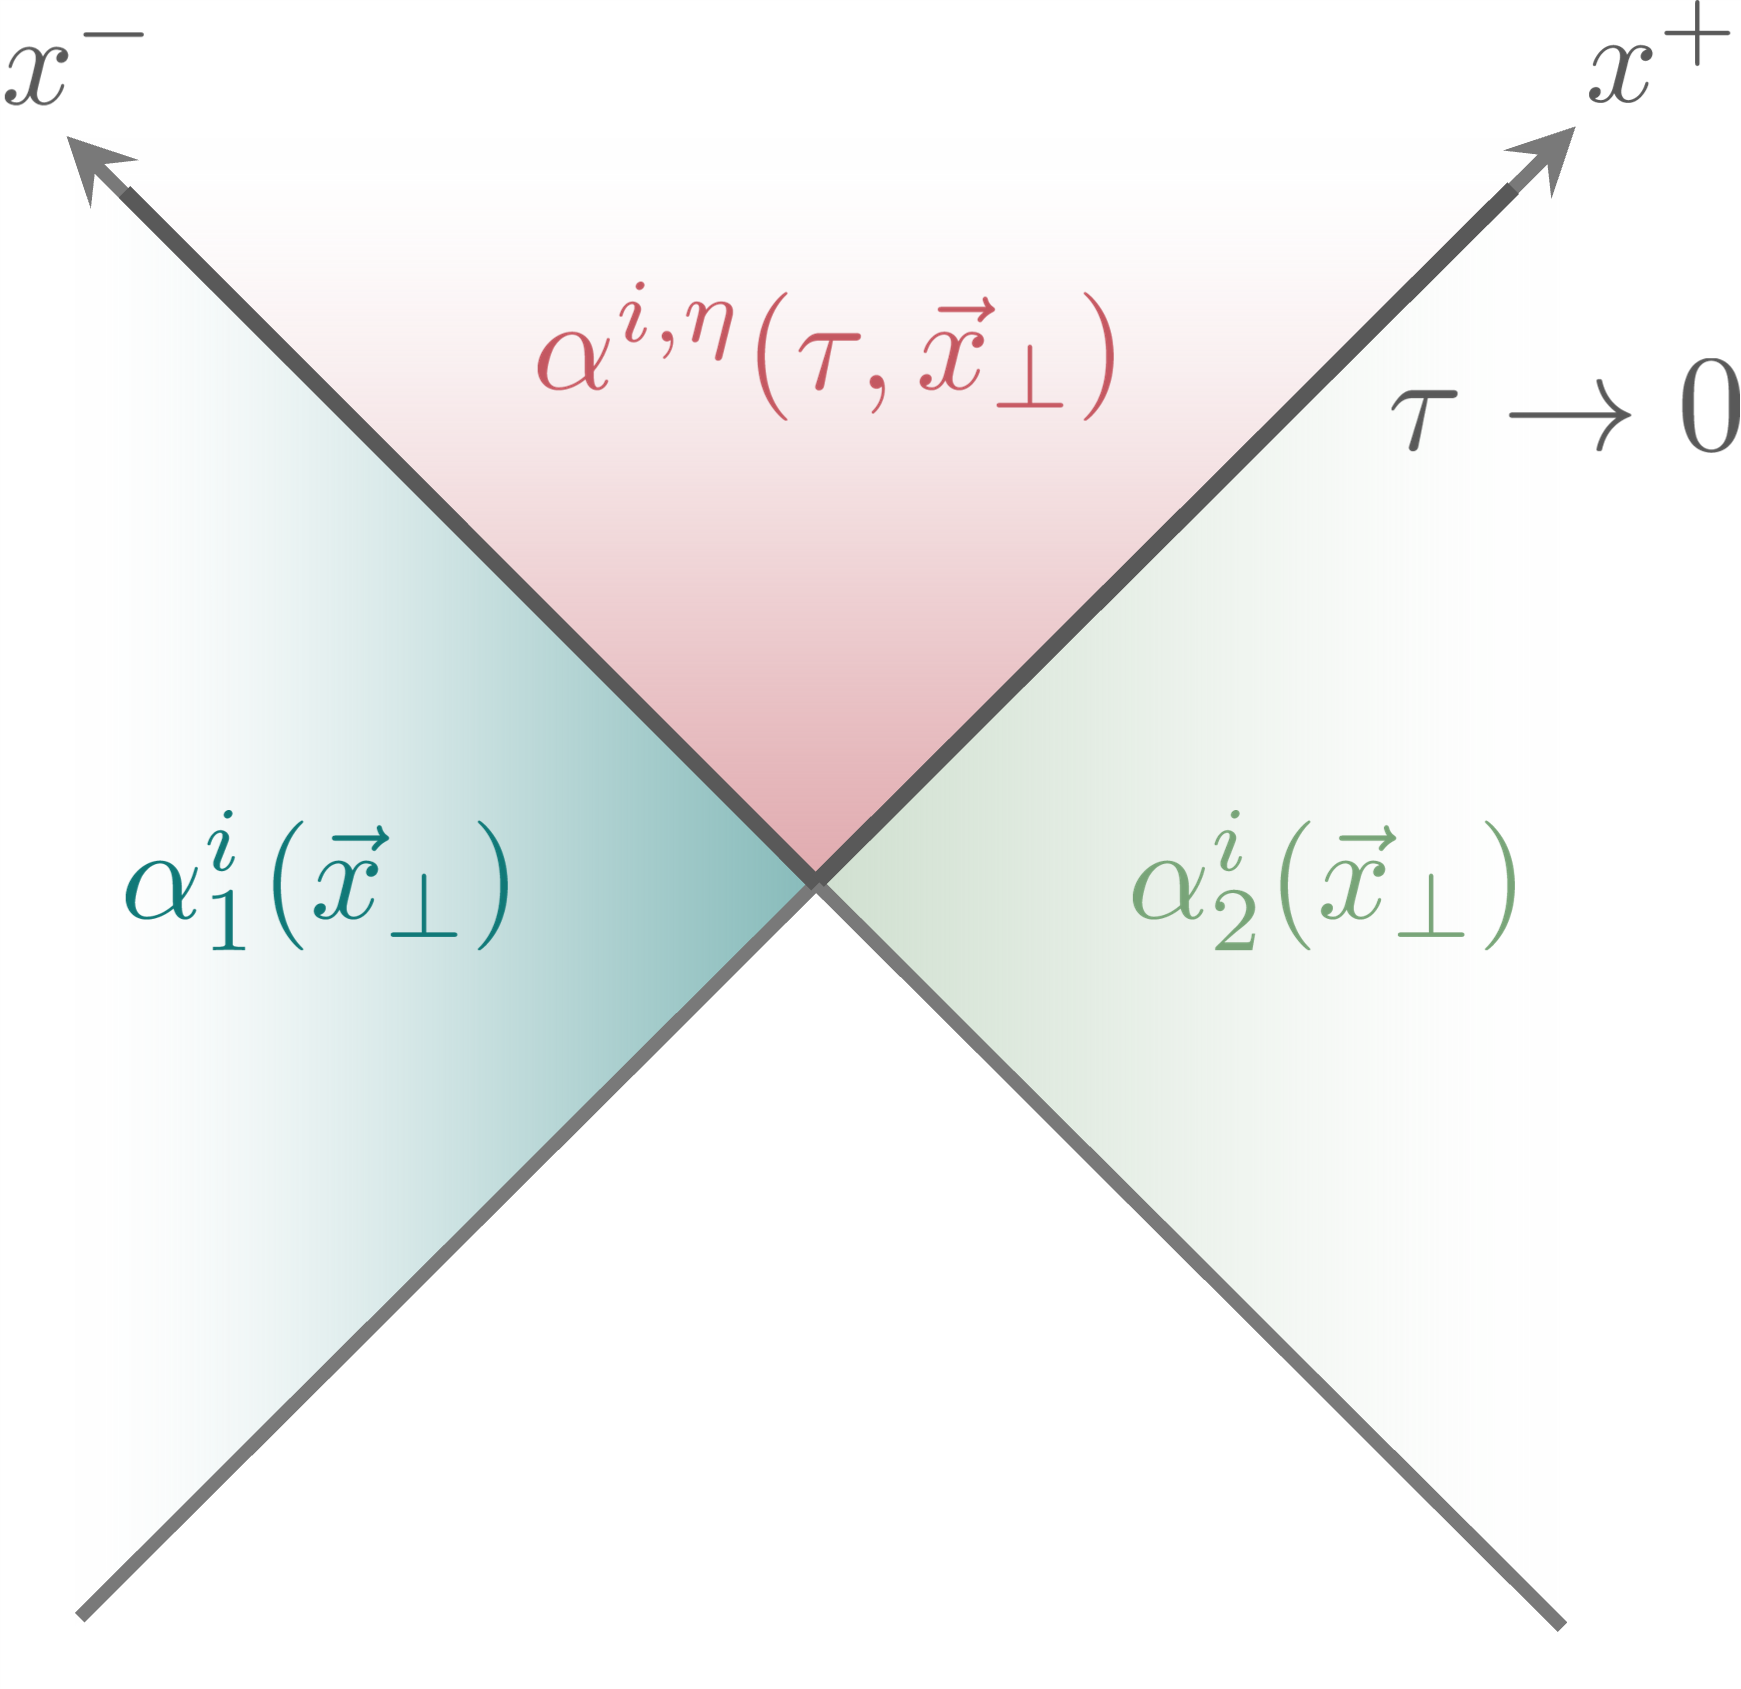
\includegraphics[width=0.85\columnwidth]{images/cgc_col.png}
            % \vspace{-0.7cm}
            \captionsetup{justification=centering}
            % \caption{\scriptsize\itshape Figure credits to D. M\"{u}ller}
        \end{figure}
        \column{.02\textwidth}
        \column{.5\textwidth}
        \vspace{0.2cm}
        \begin{center}
            {\color{customgreen}$\sbullet[0.6]$ Known CGC fields} at $\tau<0$ \\[0.1cm]
            {\color{custompink}$\sbullet[0.6]$ Unknown Glasma fields} at $\tau>0$ \\[0.5cm]
            {\scriptsize{\color{lightgray}Milne coordinates ($\tau$, $\eta$)} \\
            {\color{lightgray}$\tau=\sqrt{2 x^+x^-}$, $\eta=\ln(x^+/x^-)/2$}\\[0.4cm]
            {\color{lightgray}Boost-invariant approximation $\mathrm{fields}=\mathrm{indep}(\eta)$} \\[0.3cm]
            {\color{lightgray}Numerical solution of Yang-Mills}\\[-0.15cm] {\color{lightgray}equations $\Rightarrow$ Glasma}}
            {\footnotesize\color{red}Add references}
        \end{center}
        \column{.02\textwidth}
    \end{columns}
\end{frame}

\begin{frame}
    \frametitle{Features of glasma}
    \framesubtitle{Saturation scale, flux tubes, anisotropy}
    \begin{columns}[onlytextwidth,t]
        \column{.02\textwidth}
       \column{.44\textwidth}
       \begin{figure}
            \centering
            % 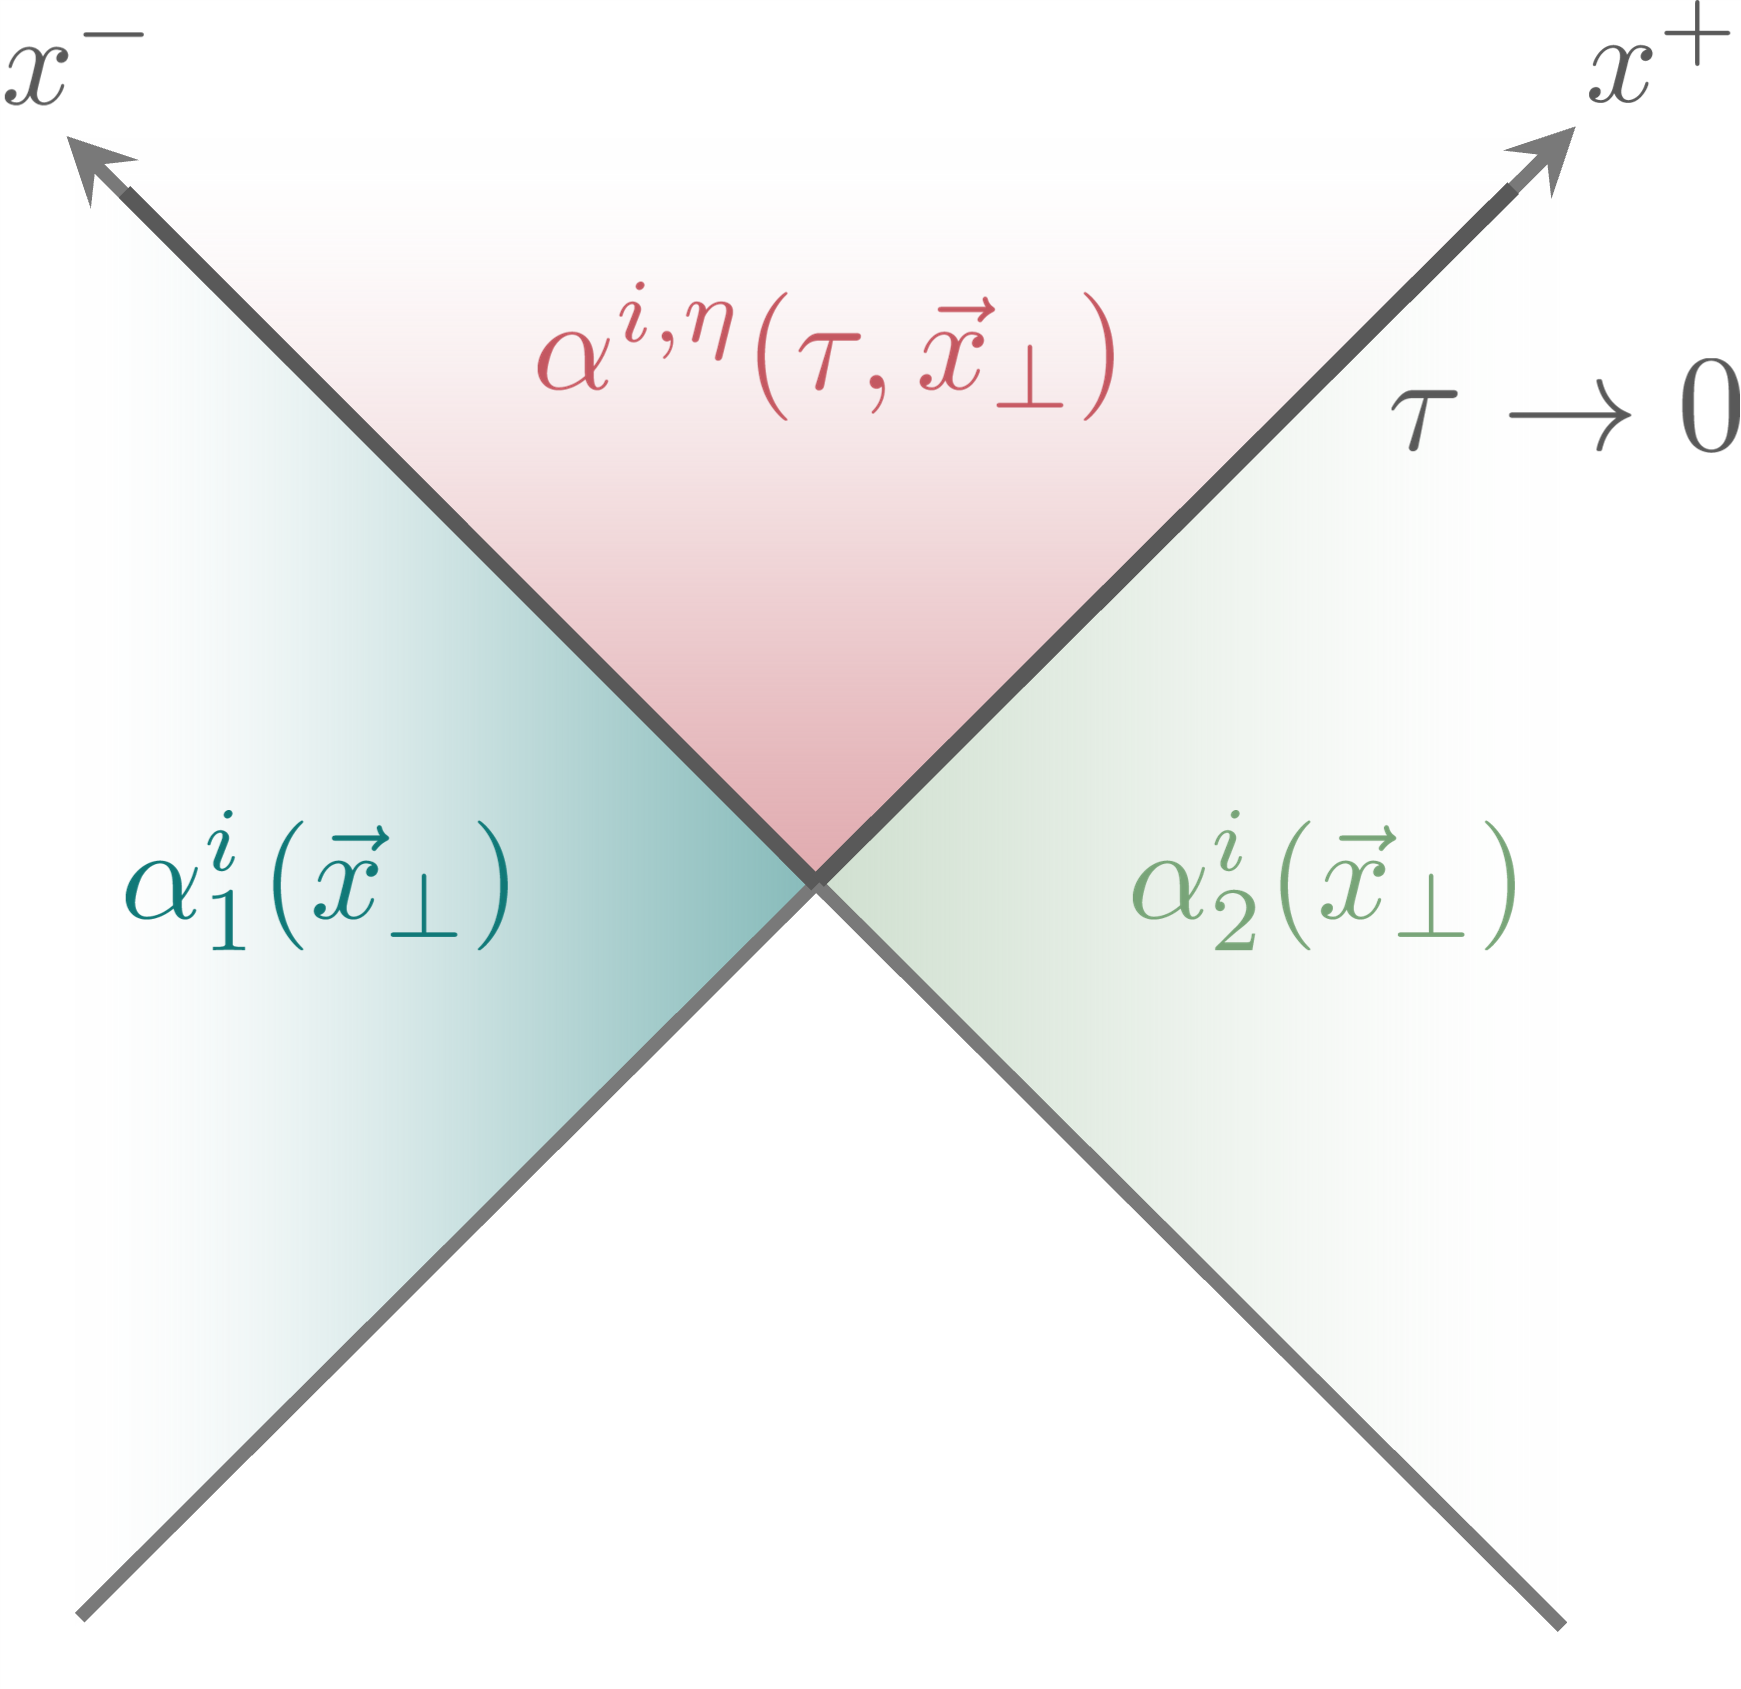
\includegraphics[width=0.85\columnwidth]{images/cgc_col.png}
            \only<1>{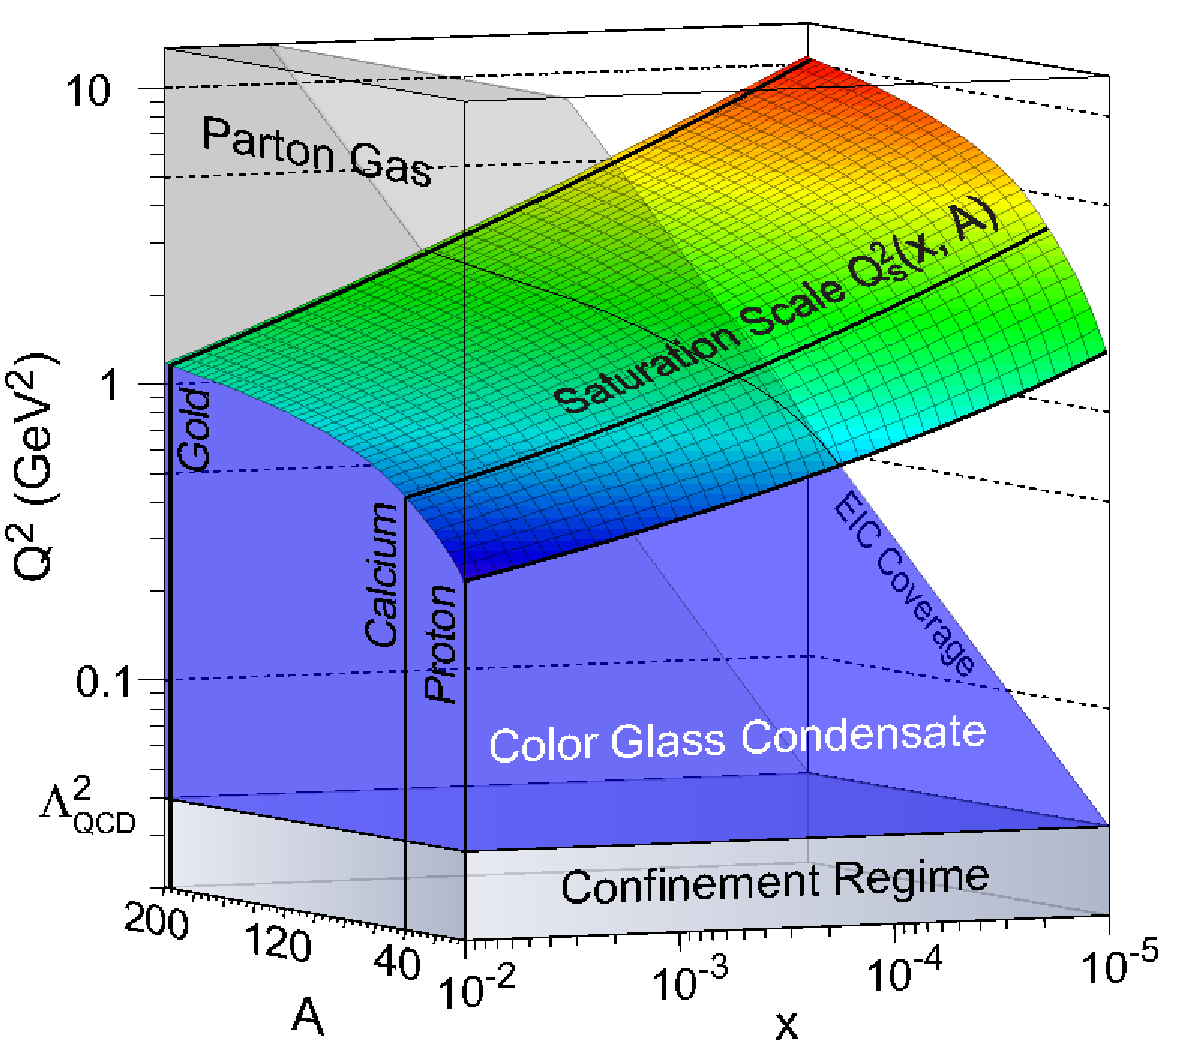
\includegraphics[width=0.75\textwidth]{images/QxA.pdf}
                \caption{\scriptsize\itshape Figure from F. Gelis \href{https://arxiv.org/abs/2102.07604}{{\color{lightgray}\texttt{[2102.07604]}}}}
            }
            \only<2>{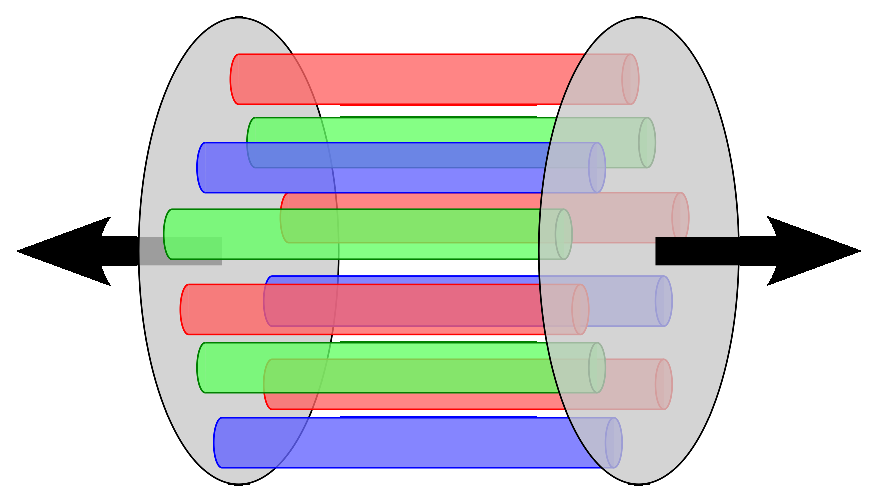
\includegraphics[width=0.75\textwidth]{images/glasma.eps}
                \caption{\scriptsize\itshape Figure from K. Fukushima \href{https://arxiv.org/abs/1603.02340}{{\color{lightgray}\texttt{[1603.02340]}}}}
            }
            % \only<3>{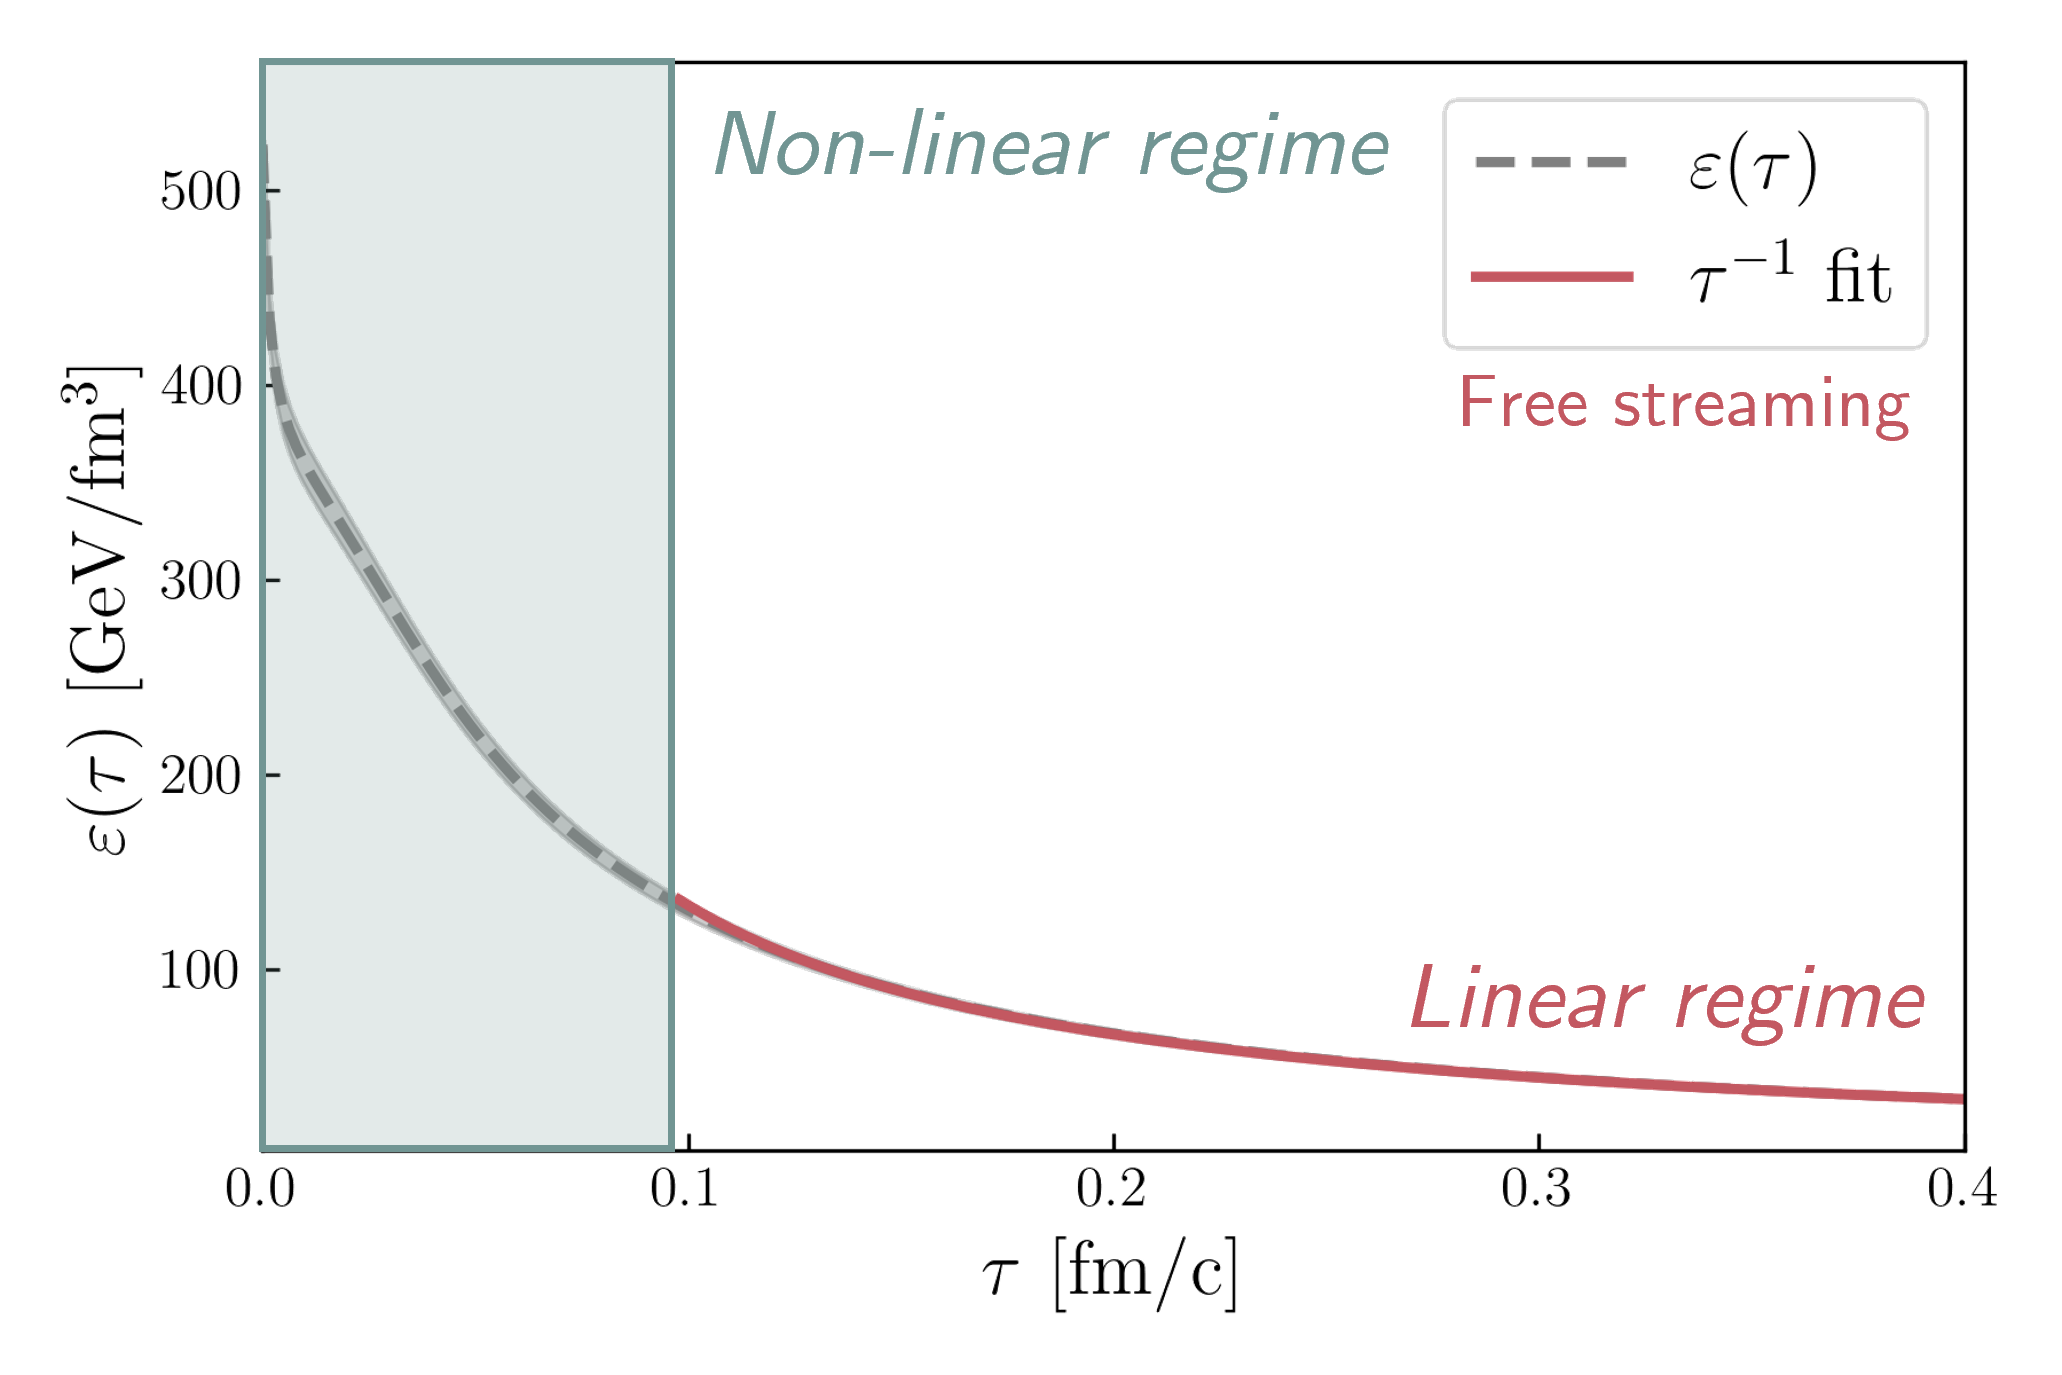
\includegraphics[width=0.9\textwidth]{images/dilute_2.png}
            %     % \caption{\scriptsize\itshape Figure from T. Lappi \href{https://arxiv.org/abs/hep-ph/0602189}{{\color{lightgray}\textit{[hep-ph/0602189]}}}}
            % }
            \only<3>{\includegraphics[width=0.75\textwidth]{images/components.eps}
                \caption{\scriptsize\itshape Figure from T. Lappi \href{https://arxiv.org/abs/hep-ph/0602189}{{\color{lightgray}\texttt{[hep-ph/0602189]}}}}
            }
            \only<4>{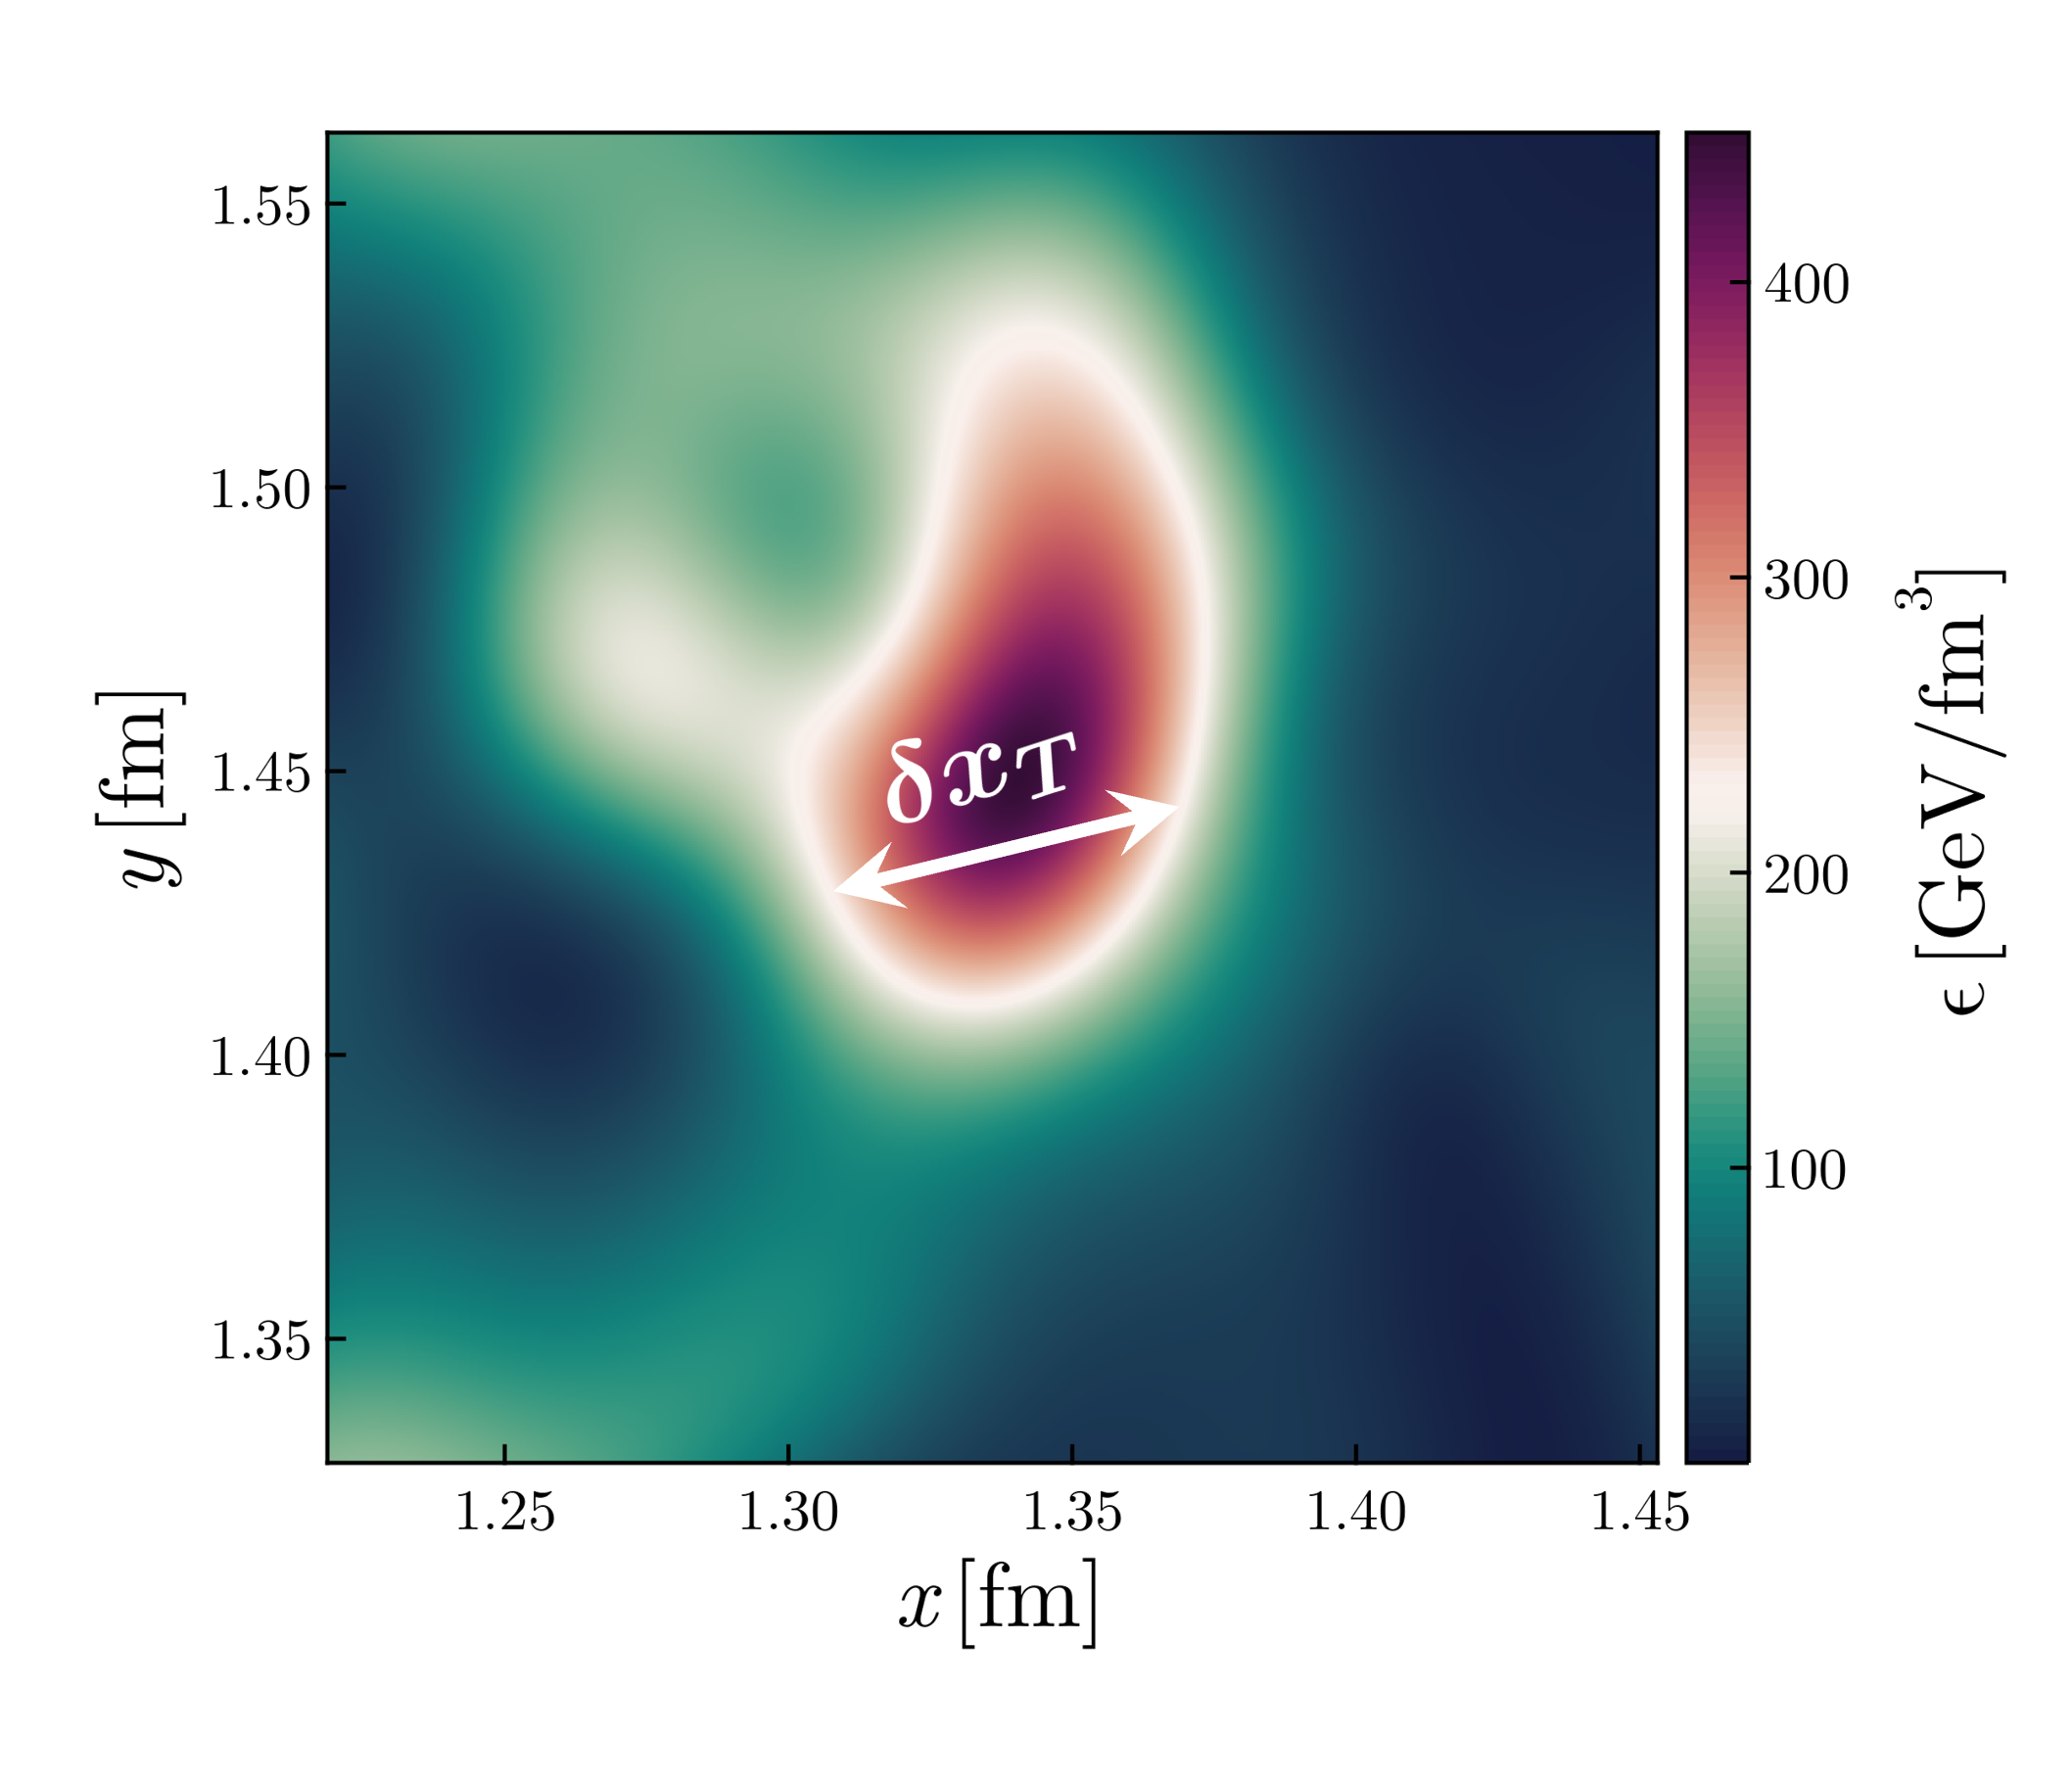
\includegraphics[width=0.9\textwidth]{images/correlation_2.png}
                % \caption{\scriptsize\itshape Figure from T. Lappi \href{https://arxiv.org/abs/hep-ph/0602189}{{\color{lightgray}\textit{[hep-ph/0602189]}}}}
            }
            % \only<5>{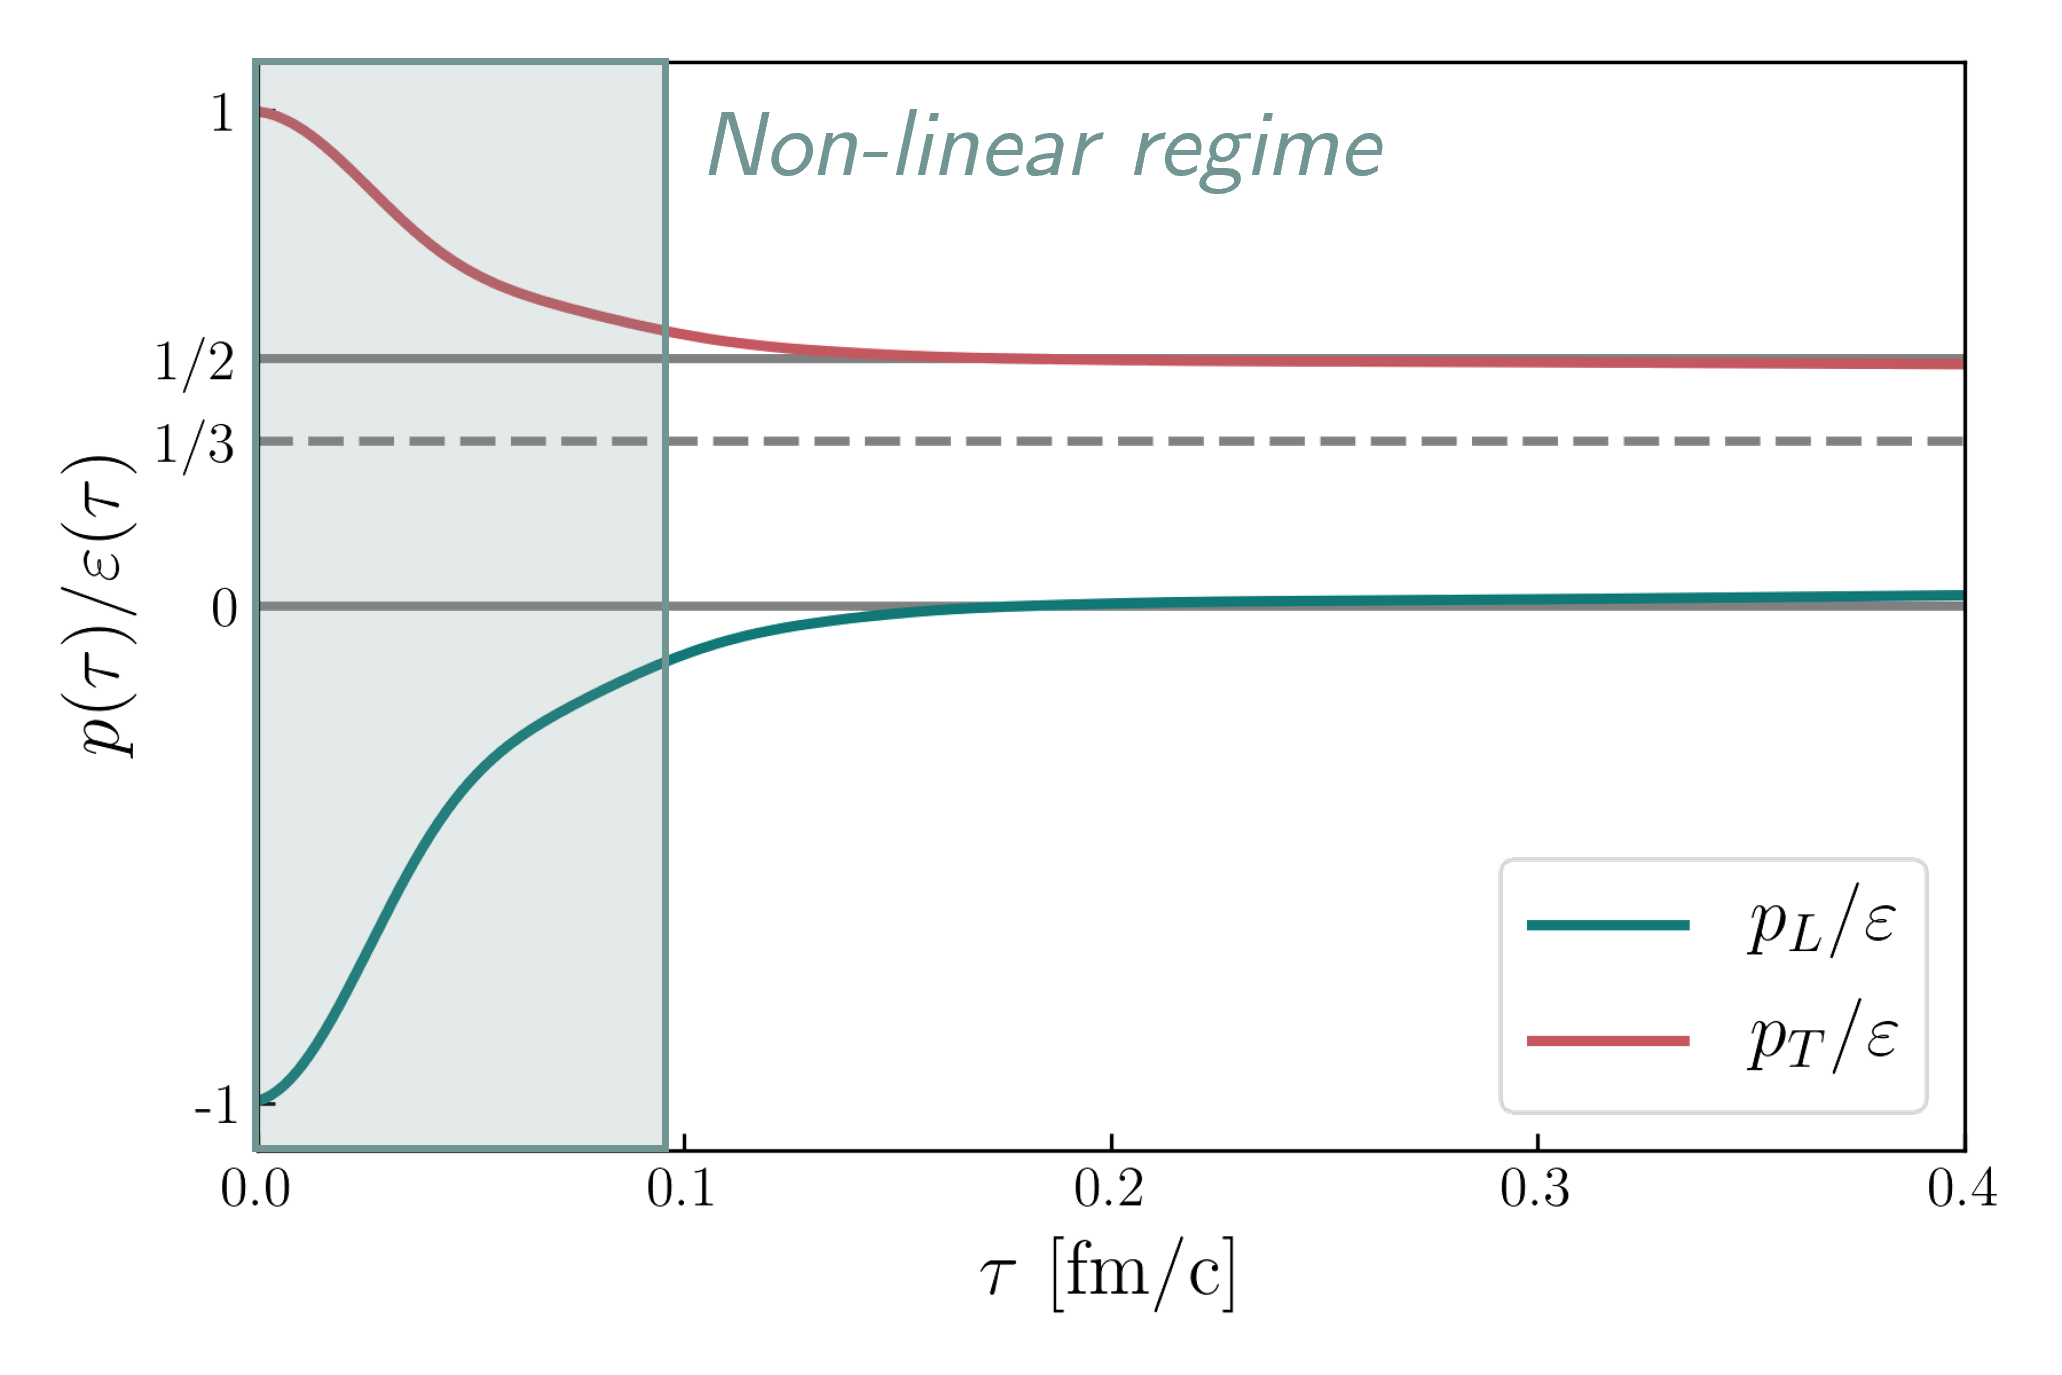
\includegraphics[width=0.9\textwidth]{images/anisotropy.png}
            \only<5>{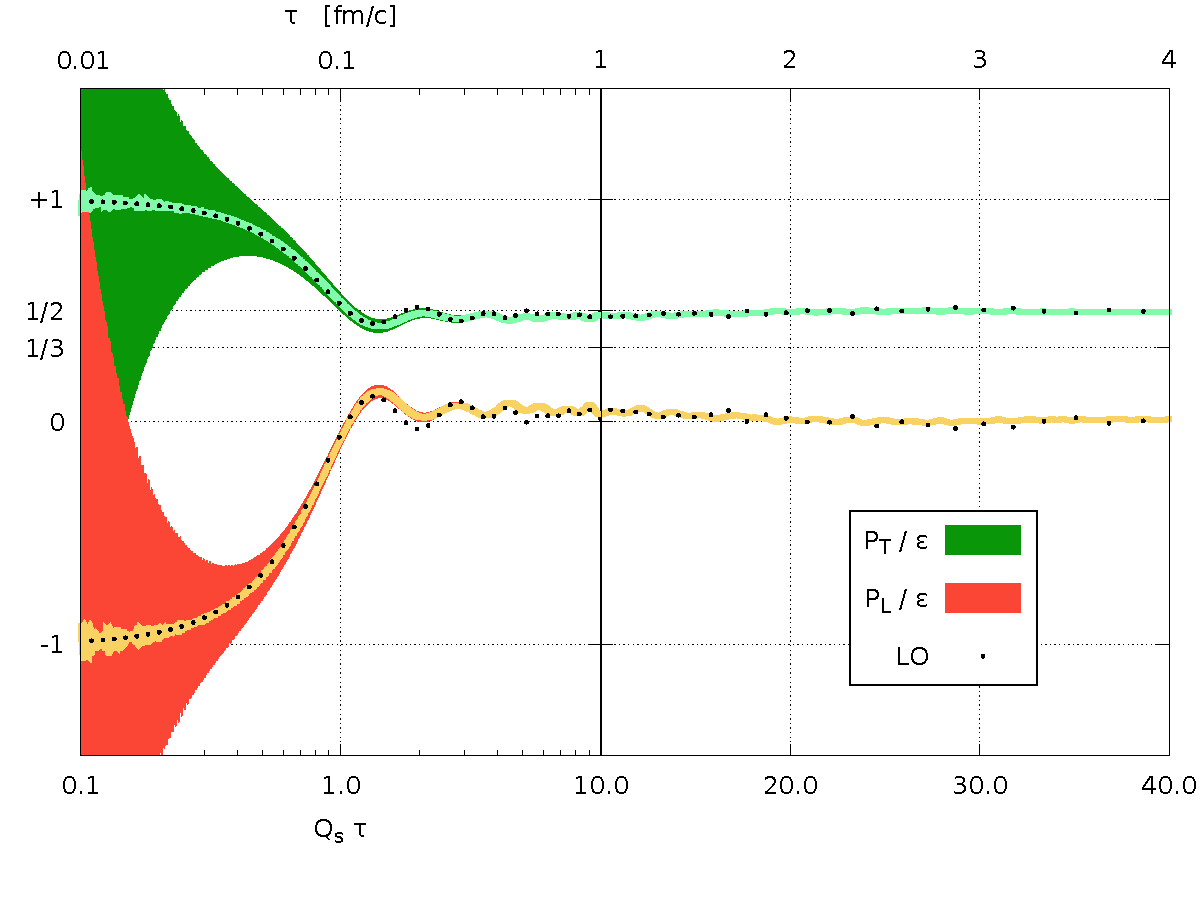
\includegraphics[width=0.9\textwidth]{images/ratio-0_1-1.pdf}
            \caption{\scriptsize\itshape Figure from F. Gelis \href{https://arxiv.org/abs/1307.2214}{{\color{lightgray}\texttt{[1307.2214]}}}}
            % \caption{\scriptsize\itshape Figure from T. Lappi \href{https://arxiv.org/abs/hep-ph/0602189}{{\color{lightgray}\textit{[hep-ph/0602189]}}}}
        }
            % \includegraphics[width=0.85\columnwidth]{images/components.eps}
            % \vspace{-0.7cm}
            % \captionsetup{justification=centering}
            % \caption{\scriptsize\itshape Figure credits to D. M\"{u}ller}
        \end{figure}
        \column{.02\textwidth}
        \column{.5\textwidth}
        \vspace{0.2cm}
        \begin{center}
            \begin{itemize}
                \onslide<1,2,3,4,5>{\item Relevant scale {\color{custompink}saturation momentum $Q_s$}}
                \onslide<2,3,4,5>{\item Initial longitudinal color flux tubes}
                \onslide<3,4,5>{\item Fields {\color{customgreen}dilute} after $\tau\simeq {\color{custompink}Q}^{-1}_{\color{custompink}s}$}
                \onslide<4,5>{\item Fields arranged in {\color{customgreen}correlation domains} of $\delta x_T \simeq {\color{custompink}Q}^{-1}_{\color{custompink}s}$}
                \onslide<5>{\item Longitudinal $\neq$ transverse pressures $\Rightarrow$ {\color{pinky}anisotropy}}
            \end{itemize}
        \end{center}
        \column{.02\textwidth}
    \end{columns}
\end{frame}

\subsection{Kinetic theory}

\setbeamertemplate{background}{
\tikz[overlay,remember picture] \node[opacity=0.1, at=(current page.center), align=center] {\\[3pt]
{\transparent{0.15}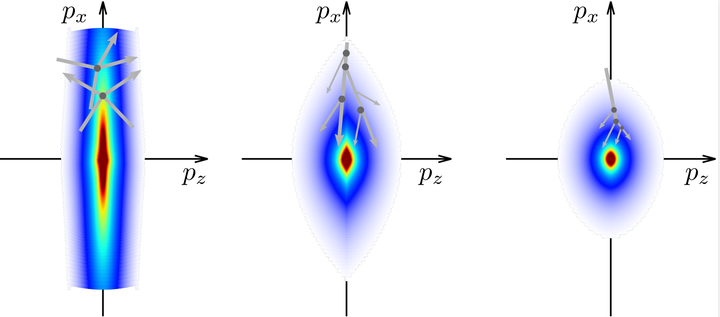
\includegraphics[height=0.6\paperheight]{images/featured_hud17e234a84b7f8be63afa171c5969276_311325_720x0_resize_lanczos_3.png}}
   \\[10pt]  
   {\transparent{0.5}\footnotesize\itshape Figure from  A. Kurkela, A. Mazeliauskas, J.-F. Paquet, S. Schlichting, D. Teaney \href{https://arxiv.org/abs/1805.00961}{{\color{lightgray}\texttt{[1805.00961]}}}}};
}
\begin{frame}[plain,noframenumbering]{}
    \begin{center}
        \vspace{1cm}
        {\large\color{normal}Next stages of pre-equilibrium}\\[0.3cm]
        {\huge\color{destacado}Effective kinetic theory}
    \end{center}
\end{frame}
\setbeamertemplate{background}{}

\setbeamertemplate{background}{
\tikz[overlay,remember picture] \node[at=(current page.center), align=center] {\\[40pt]
{\transparent{1}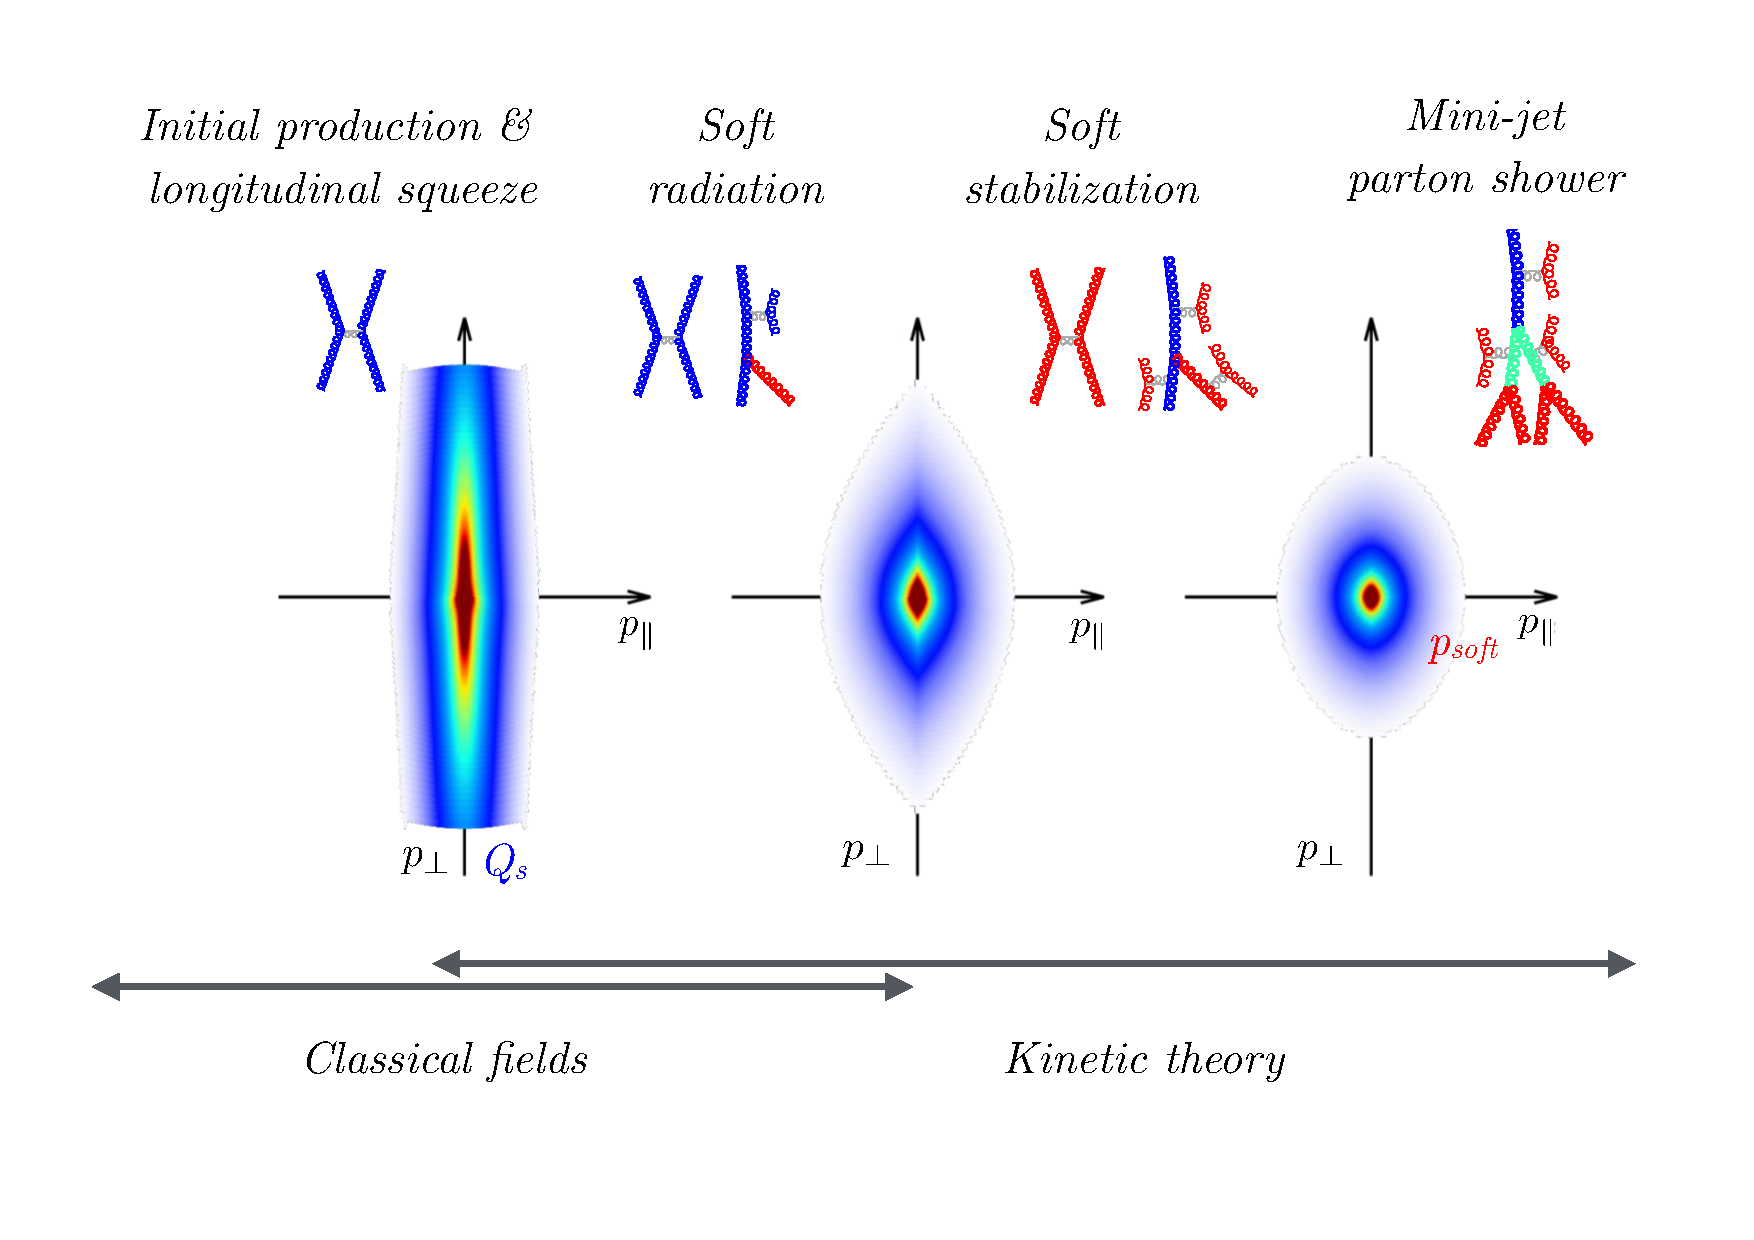
\includegraphics[height=0.65\paperheight]{images/CARTOON_BUP_SS.pdf}}
   \\[10pt]  
   {\transparent{1}\footnotesize\itshape Figure from  S. Schlichting, D. Teaney \href{https://arxiv.org/abs/1908.02113}{{\color{lightgray}\texttt{[1908.02113]}}}}};
}
\begin{frame}
    \frametitle{Bottom-up thermalization}
    \framesubtitle{Equilibration at weak coupling}
\end{frame}
\setbeamertemplate{background}{}

\begin{frame}
    \frametitle{Effective kinetic theory}
    \framesubtitle{\`{A} la AMY\footnote{\scriptsize Arnold, Moore, Yaffe \href{https://iopscience.iop.org/article/10.1088/1126-6708/2003/01/030}{{\color{customblue}\texttt{[JHEP01(2003)]}}}} and KZ\footnote{\scriptsize Kurkela, Zhu \href{https://journals.aps.org/prl/abstract/10.1103/PhysRevLett.115.182301}{{\color{customblue}\texttt{[Phys.Rev.Lett.115(2015)]}}}}}
    \begin{columns}[onlytextwidth,t]
        \column{.02\textwidth}
       \column{.46\textwidth}
       \begin{figure}
            \centering
            \captionsetup{justification=centering}
            \caption{\scriptsize Trajectories for different initial conditions\footnotemark[2]}
            \includegraphics[width=0.85\textwidth]{images/cdplot_4.eps}
        \end{figure}
        \column{.02\textwidth}
        \column{.5\textwidth}
        \vspace{0.2cm}
        \begin{itemize}
            % \item Gluon distribution function $f(t,\boldsymbol{p})$
            \item Boltzmann equation\\
                \renewcommand{\eqnhighlightheight}{\vphantom{\mathcal{D}_\mu}\mathstrut}\begin{equation*}
                -\frac{\mathrm{d}}{\mathrm{d} \tau}\eqnmark[pinky]{fp}{f_{\boldsymbol{p}}}=\Big(
                \eqnmark[ming]{c12}{\mathcal{C}_{1 \leftrightarrow 2}}+ \eqnmark[ming]{c22}{\mathcal{C}_{2 \leftrightarrow 2}}+ \eqnmark[starrysecond]{cexp}{\mathcal{C}_{\mathrm{exp}}}\Big)({\color{pinky}f_{\boldsymbol{p}}})
                \end{equation*}
                \annotate[yshift=-2.2em]{below, right}{fp}{\scriptsize distribution function}
                \annotatetwo[yshift=+1em]{above}{c12}{c22}{\scriptsize collision terms}
                \annotate[yshift=-0.7em]{below, left}{cexp}{\scriptsize longitudinal expansion}
                \\[20pt]
            {\footnotesize \item Soft scale $m_D$ $\ll$ hard scale $Q_s$
            \item Overoccupied $f\sim 1/\alpha_s$ at $Q_s\tau\sim 1$
            \item Boost-invariance $p_z\ll p_T$}
        \end{itemize}
        \column{.02\textwidth}
    \end{columns}
\end{frame}

\begin{frame}
    \frametitle{Stages of bottom-up}
    \framesubtitle{Classical fields, soft particles, energy loss}
    \begin{columns}[onlytextwidth,t]
        \column{.02\textwidth}
       \column{.44\textwidth}
       \begin{figure}
            \centering
            \captionsetup{justification=centering}
            \only<1>{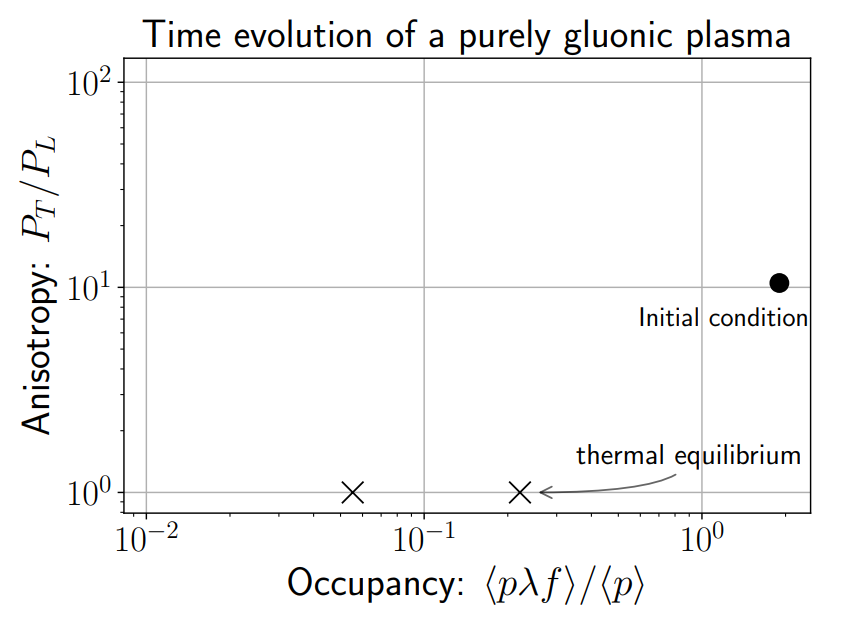
\includegraphics[width=0.95\textwidth]{images/Screenshot from 2024-08-23 15-55-35.png}}
            \only<2>{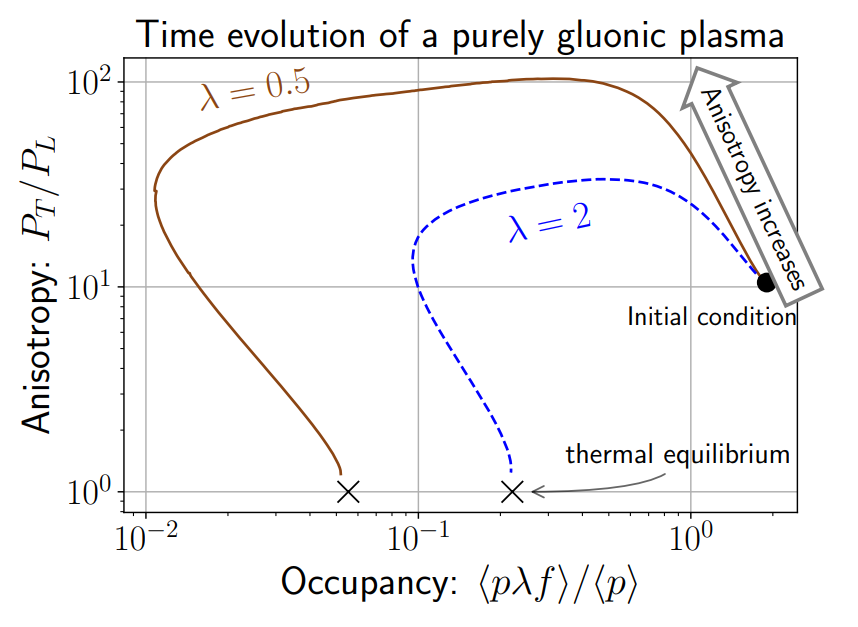
\includegraphics[width=0.95\textwidth]{images/Screenshot from 2024-08-23 15-55-47.png}}
            \only<3>{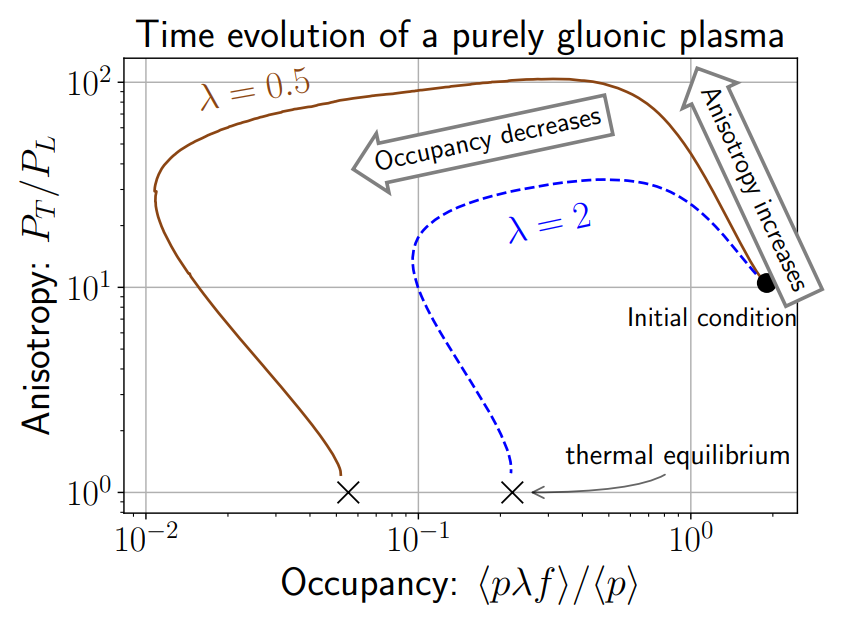
\includegraphics[width=0.95\textwidth]{images/Screenshot from 2024-08-23 15-55-53.png}}
            \only<4>{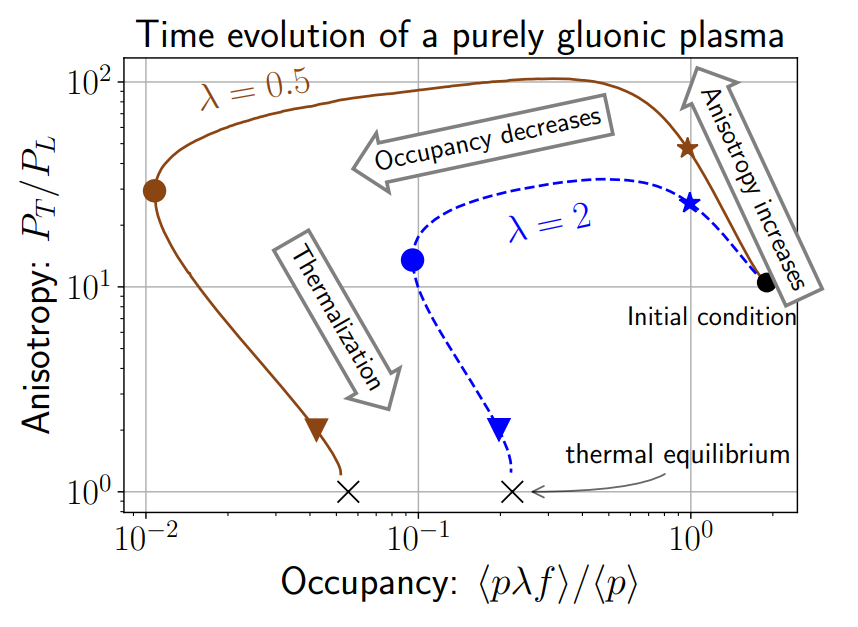
\includegraphics[width=0.95\textwidth]{images/Screenshot from 2024-08-23 15-56-03.png}}
            \only<5>{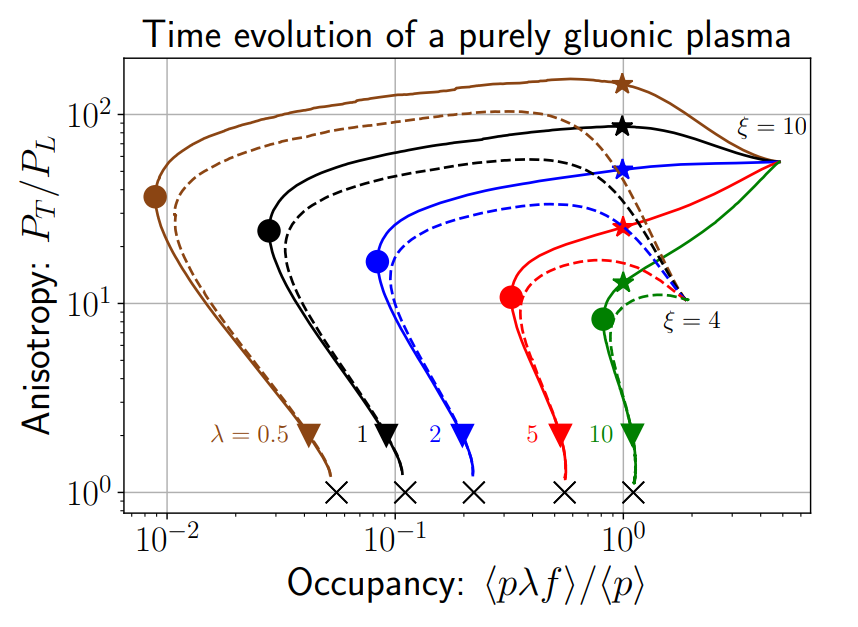
\includegraphics[width=0.95\textwidth]{images/Screenshot from 2024-08-23 15-56-07.png}}
        \end{figure}
        \column{.02\textwidth}
        \column{.5\textwidth}
        \vspace{0.2cm}
        \begin{center}
            \begin{itemize}
                \onslide<1,2,3,4,5>{\item Stage $\boldsymbol{\circ}$\\ 
                Overoccupied gluon fields\\
                Anisotropy $\xi$, coupling $\lambda=4\pi N_c\alpha_s$}
                \onslide<2,3,4,5>{\item {\color{ming}Stage $\boldsymbol{\star}$} \\
                Maximum anisotropy, hard modes}
                \onslide<3,4,5>{\item {\color{ming}Stage $\bullet$} \\
                Minimum occupancy, bath of soft modes}
                \onslide<4,5>{\item {\color{ming}Stage $\mathsmaller{\blacktriangledown}$} \\
                Almost isotropic, hard modes radiated}
                \onslide<5>{\\ Thermalization $\tau_{\mathrm{BMSS}}\sim \alpha_s^{-13/5}Q_s^{-1}$}
            \end{itemize}
        \end{center}
        \column{.02\textwidth}
    \end{columns}
\end{frame}

\begin{frame}[noframenumbering]
    \frametitle{Stages of bottom-up}
    % \framesubtitle{Many studies}
    \begin{center}
       \begin{figure}
            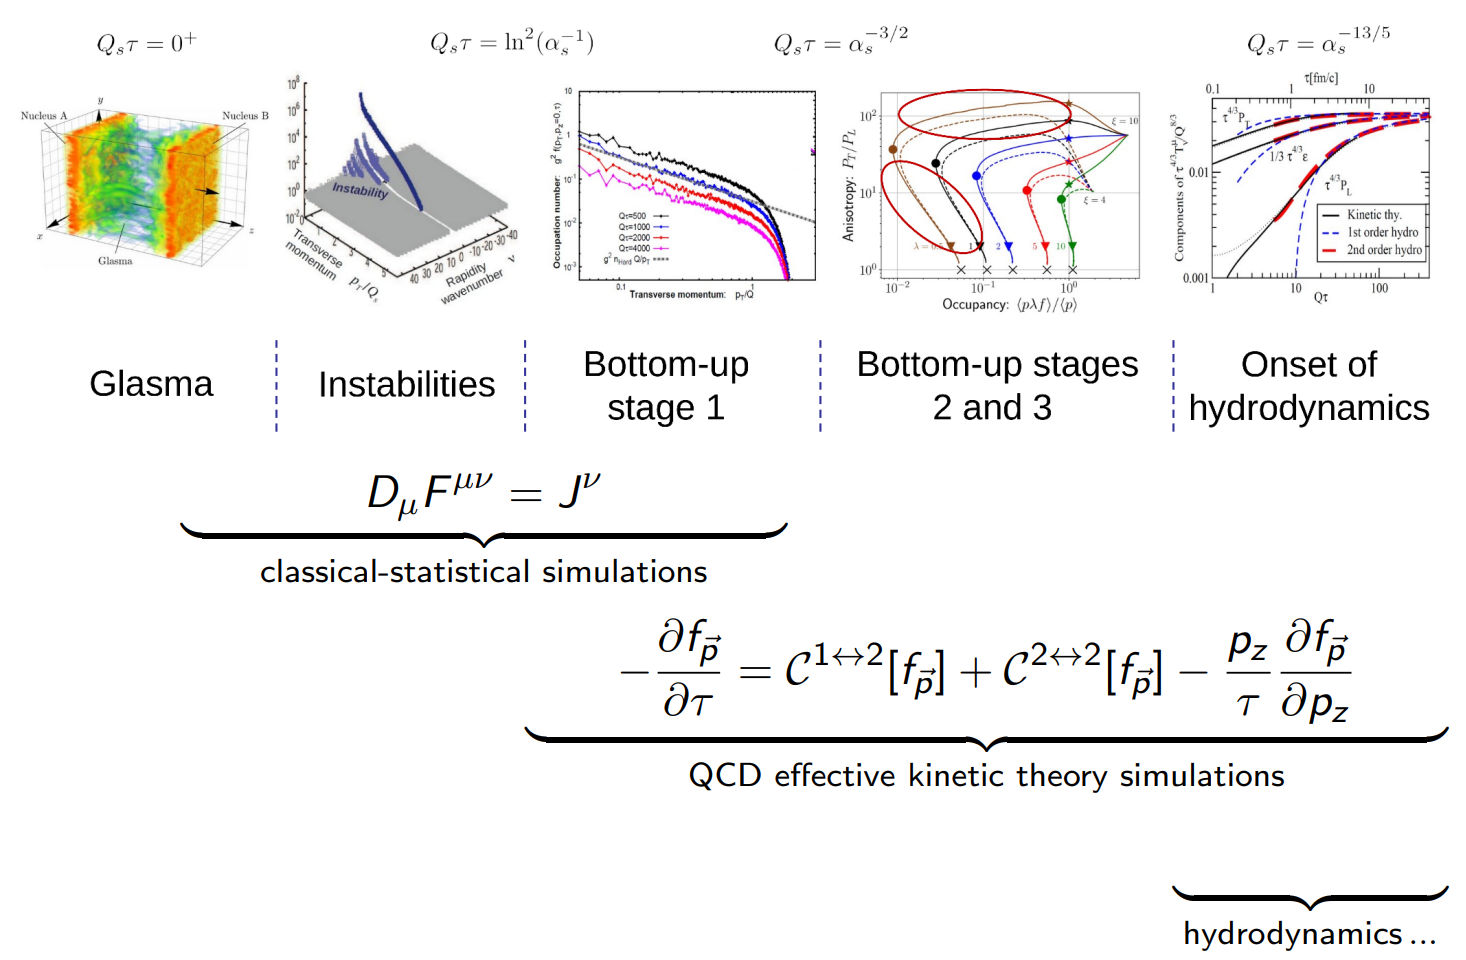
\includegraphics[width=1.4\textheight]{images/Screenshot from 2024-08-23 16-32-50.png}
        \end{figure}
        {\color{red}Add references}
    \end{center}
\end{frame}

% \setbeamertemplate{background}{
% \tikz[overlay,remember picture] \node[at=(current page.center), align=center] {\\[40pt]
% {\transparent{0.2}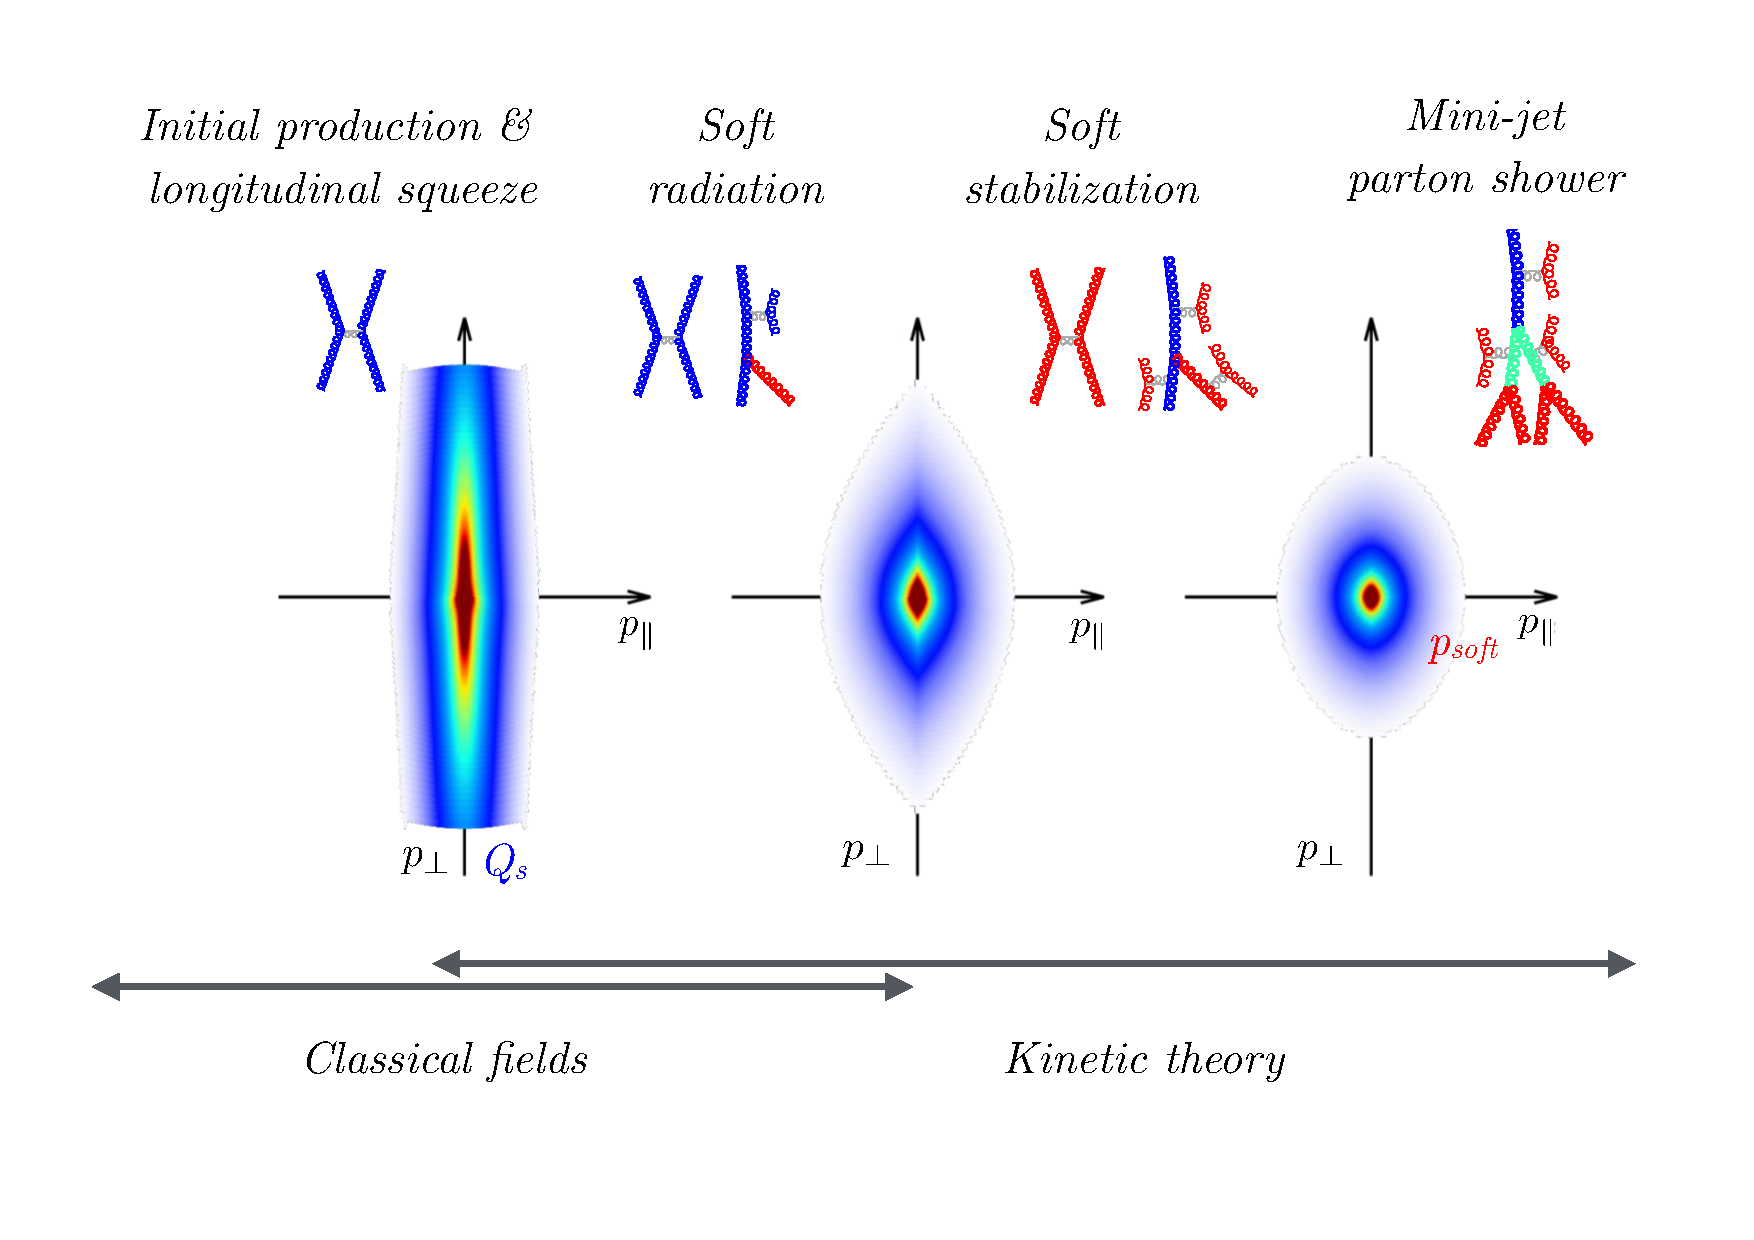
\includegraphics[height=0.65\paperheight]{images/CARTOON_BUP_SS.pdf}}
%    \\[10pt]  
%    {\transparent{5}\footnotesize\itshape Figure from  S. Schlichting, D. Teaney \href{https://arxiv.org/abs/1908.02113}{{\color{lightgray}\texttt{[1908.02113]}}}}};
% }
% \begin{frame}
%     \frametitle{Bottom-up thermalization}
%     \framesubtitle{Equilibration at weak coupling}
%     \begin{center}
%         {\huge Weak coupling parametric estimate}\\[20pt]
%         {\footnotesize\itshape Other frameworks for pre-equilibrium dynamics are not included in this talk\\
%         {\color{red}Add references}}
%     \end{center}
% \end{frame}
% \setbeamertemplate{background}{}


%%%%%%%%%%%%%%%%%%%%%%%%%%%%%%%%%%%%%%%%%%%
%%%%%%%%%%%%%%%% SECTION 3 %%%%%%%%%%%%%%%%
%%%%%%%%%%%%%%%%%%%%%%%%%%%%%%%%%%%%%%%%%%%

\section{{\color{jyublue}Heavy quarks} in pre-equilibrium}

\setbeamertemplate{background}{
\tikz[overlay,remember picture] \node[opacity=0.1, at=(current page.center), align=center] {
    % \\[-20pt]
    \\[45pt]
{\transparent{0.3}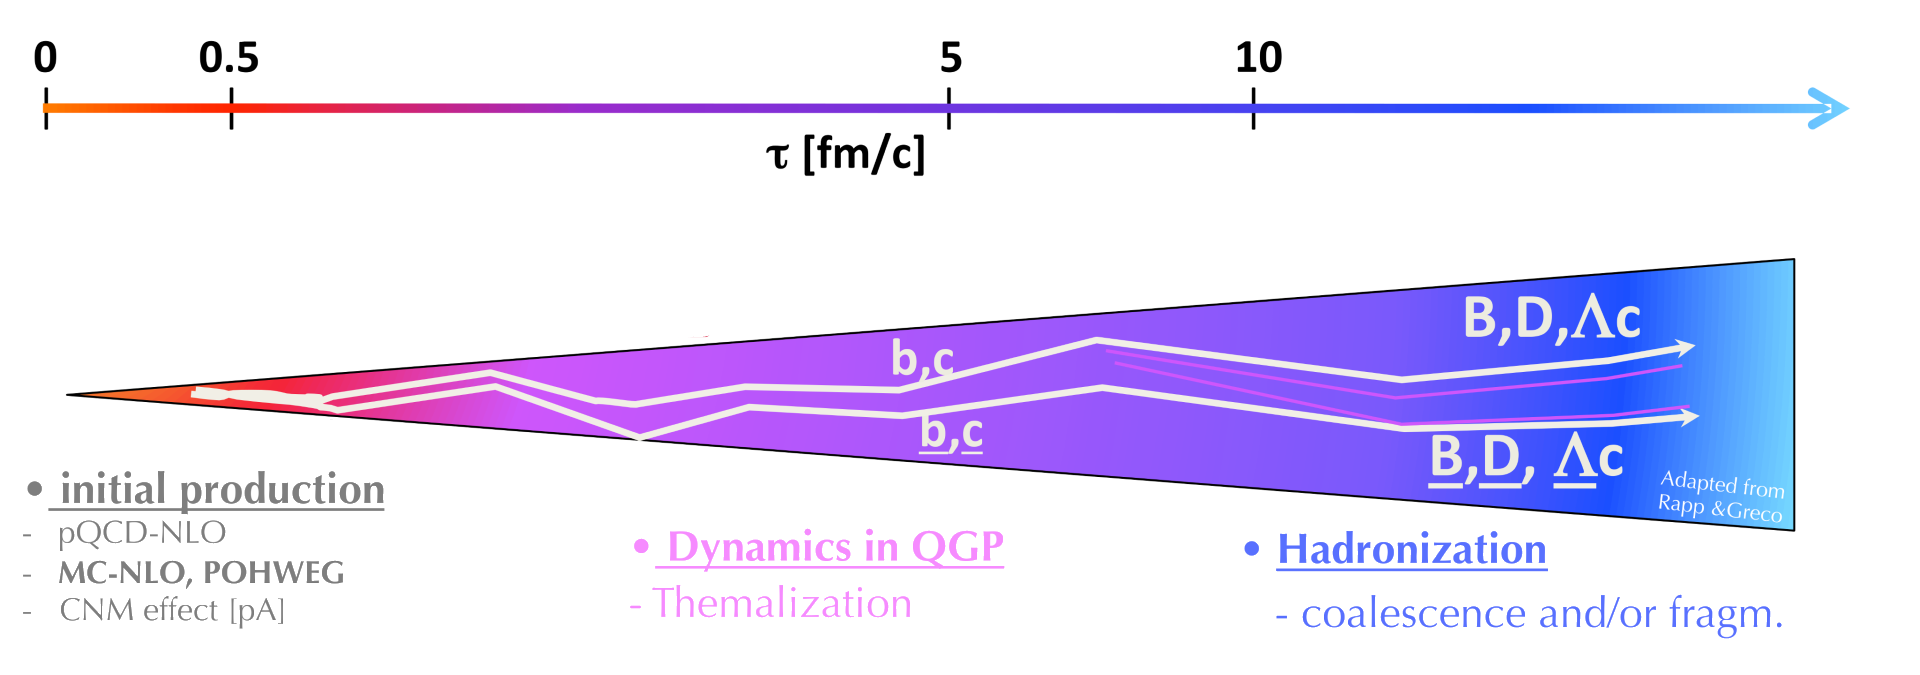
\includegraphics[height=0.6\paperheight]{images/Greco-HF-Theory-HP2020-v-5_edit.png}}
   \\[10pt]  
   {\transparent{0.3}\footnotesize\itshape Figure credits to V. Greco}};
}
\begin{frame}[plain,noframenumbering]{}
    \begin{center}
        \vspace{1cm}
        {\huge\color{destacado}Heavy quarks in pre-equilibrium}
    \end{center}
\end{frame}
\setbeamertemplate{background}{}


\subsection{Glasma}

\setbeamertemplate{background}{
\tikz[overlay,remember picture] \node[opacity=0.1, at=(current page.center), align=center] {\\[10pt]
{\transparent{0.1}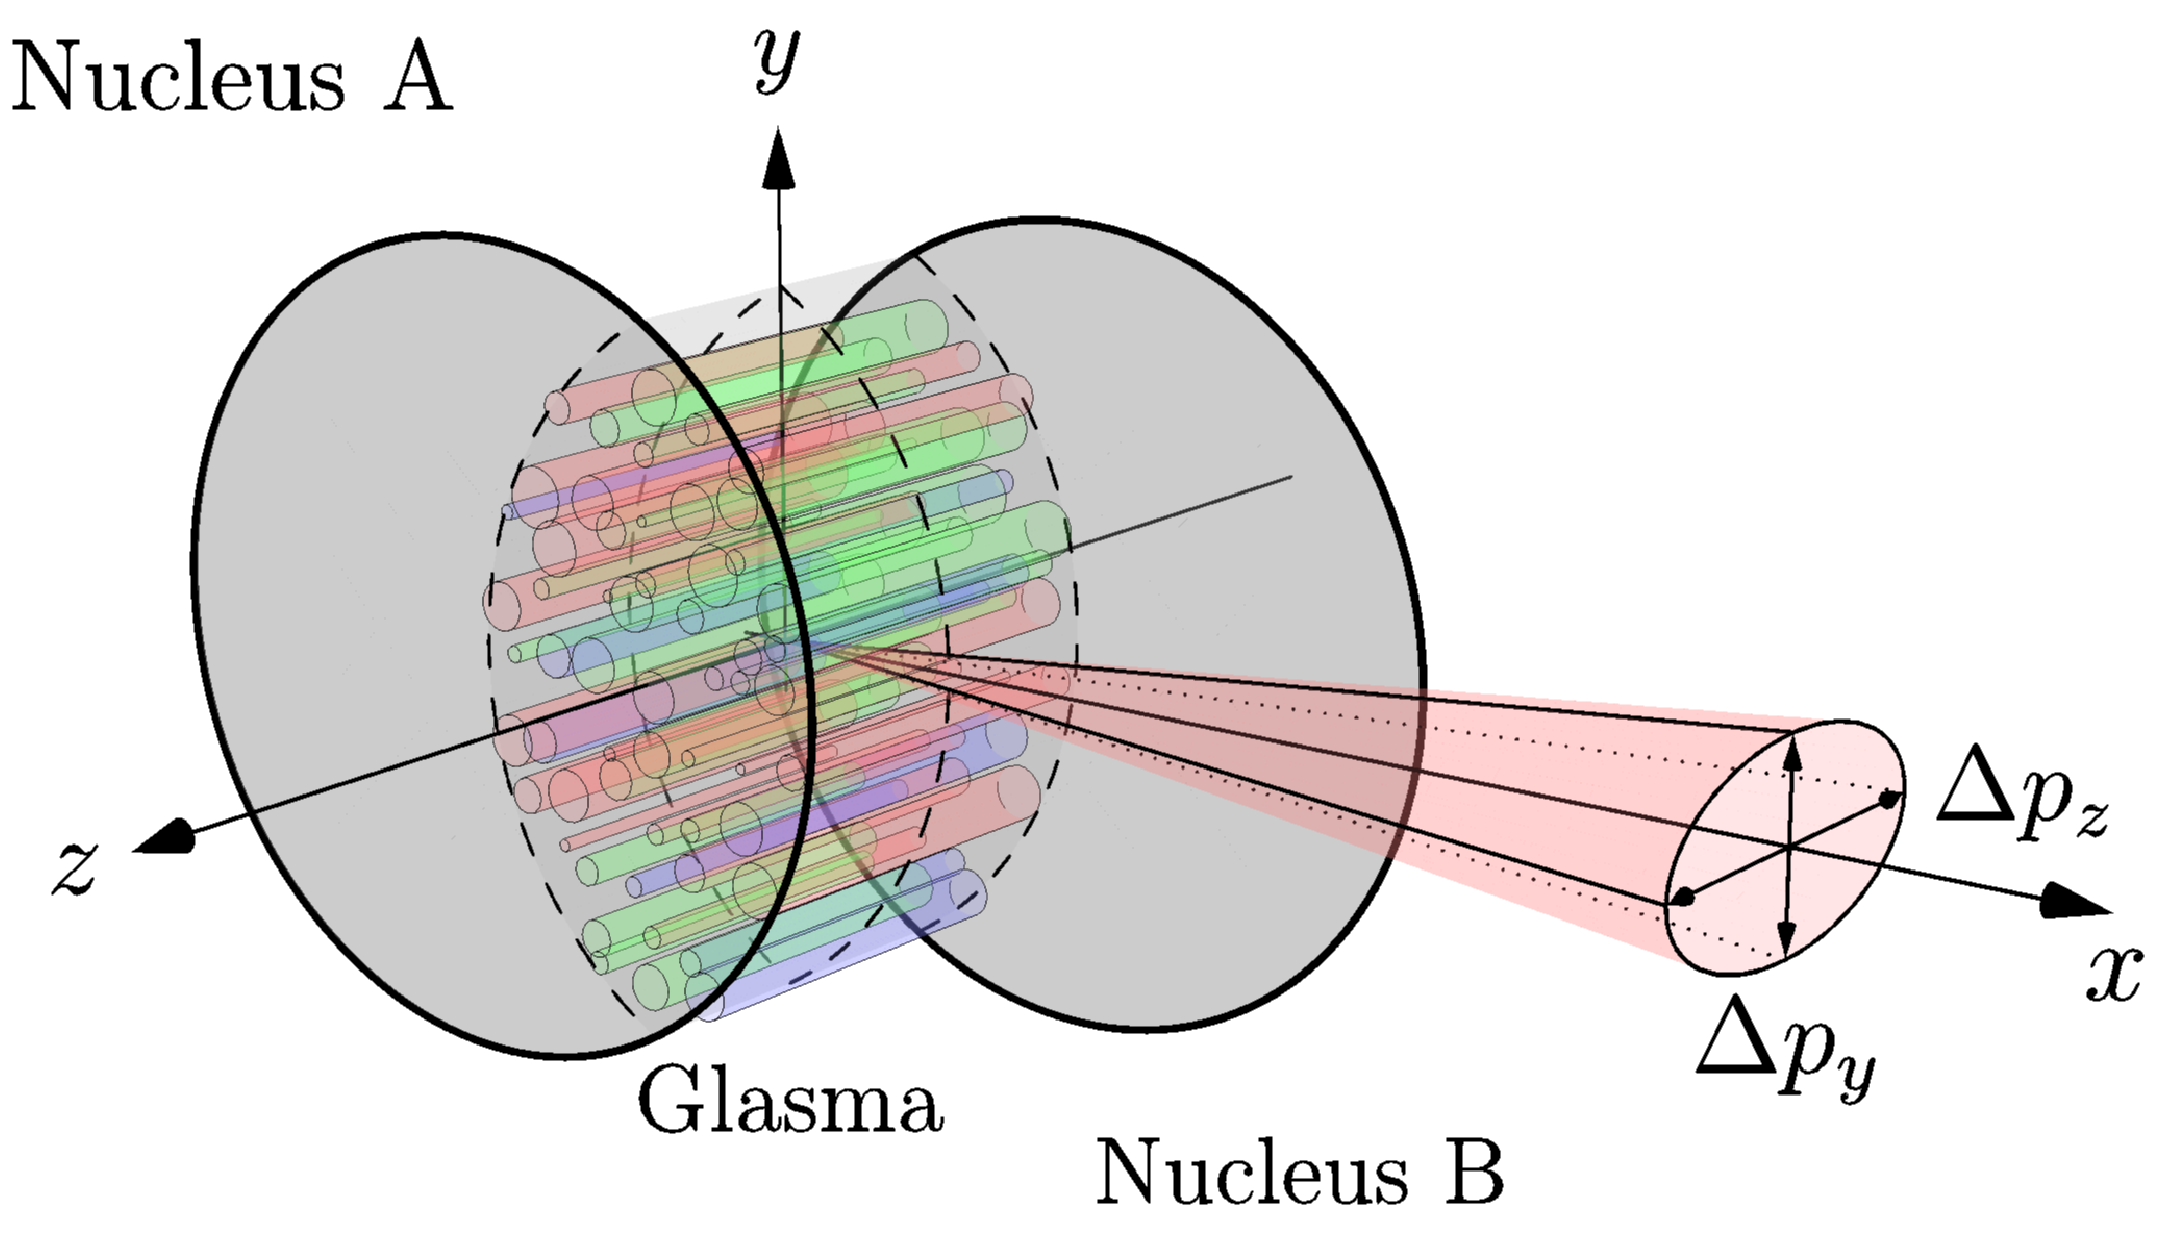
\includegraphics[height=0.7\paperheight]{images/momentum_broadening_flipped.pdf}}
   \\[10pt]  
   {\transparent{0.3}\footnotesize\itshape Figure from  A. Ipp, D. Müller, D. Schuh \href{https://arxiv.org/abs/2009.14206}{{\color{lightgray}\texttt{[2009.14206]}}}}};
}

\setbeamertemplate{itemize item}{\raisebox{0.2em}{\scalebox{0.7}{${\color{normal}\blacktriangleright}$}}} 

\begin{frame}[plain,noframenumbering]{}
    \begin{center}
        \vspace{1cm}
        {\large\color{normal}Initial stage of pre-equilibrium}\\[0.3cm]
        {\huge\color{destacado}Heavy quarks in glasma}\\[0.3cm]
        {\large\color{normal}
        \begin{center}
            % \begin{minipage}{0.45\textwidth}
            % \begin{itemize}
            %     \item Momentum broadening $\langle \delta p^2\rangle$
            %     \item Transport coefficient $\kappa$
            %     \item Observables $R_{AA}$, $v_2$, $\mathcal{C}(\Delta\phi)$
            % \end{itemize}
            % \end{minipage}
            \begin{columns}
                \begin{column}{0.066\textwidth}\end{column}
                \begin{column}{0.45\textwidth}
                    \centering
                    \\[10pt]
                    \setbeamertemplate{itemize item}{\raisebox{0.2em}{\scalebox{0.7}{${\color{pinky}\blacktriangleright}$}}} 
                    {\Large\color{pinky} Quantities}
                    \begin{itemize}
                        \item Momentum broadening $\langle \delta p^2\rangle$
                        \item Transport coefficient $\kappa$
                        \item Observables $R_{AA}$, $v_2$, $\mathcal{C}(\Delta\phi)$
                    \end{itemize}
                \end{column}
                \begin{column}{0.066\textwidth}\end{column}
                \begin{column}{0.35\textwidth}
                    \centering
                    \setbeamertemplate{itemize item}{\raisebox{0.2em}{\scalebox{0.7}{${\color{ming}\blacktriangleright}$}}} 
                    {\Large\color{ming} Approaches}
                    \begin{itemize}
                        \item Numerical trajectories
                        \item Correlator method
                    \end{itemize}
                \end{column}
                \begin{column}{0.066\textwidth}\end{column}
            \end{columns}
        \end{center}
        }
        % \\[0.3cm]
    \end{center}
\end{frame}
\setbeamertemplate{background}{}

\begin{frame}
    \frametitle{Particles in Yang-Mills fields}
    \framesubtitle{Wong's equations of motion}
        \setbeamertemplate{itemize item}{\raisebox{0.2em}{\scalebox{0.7}{${\color{ming}\blacktriangleright}$}}} 
        \begin{itemize}
            \item \begin{center}{\color{ming}Approach}: {\color{ming}numerical trajectories} of classical particles in glasma fields \end{center}
        \end{itemize} 
   \begin{center}
       Wong's equations $\leftrightarrow$ classical equations of motion for particles $({\color{customblue}x^\mu},{\color{customred}p^\mu},{\color{customyellow}Q})$ \\
    evolving in a Yang-Mills background field ${\color{starrysecond}A^\mu}$
   \end{center} 
        \vspace{1cm}
        \renewcommand{\eqnhighlightheight}{\vphantom{x}}
        \begin{equation*}
            \frac{\d}{\d\hspace{-0.1cm}\eqnmark[destacado]{tau}{\boldsymbol{\tau}}\hspace{-0.2cm}}\eqnmark[customblue]{xmu}{x^\mu}=\frac{{\color{customred}p^\mu}}{\eqnmark[destacado]{m}{m}},\qquad \eqnmark[destacado]{Ddtau}{\frac{\mathrm{D}}{\d\boldsymbol{\tau}}}\hspace{-0.2cm}\eqnmark[customred]{pmu}{p^\mu}=2\hspace{-0.1cm}\eqnmark[destacado]{g}{g}\hspace{-0.1cm}\tr{{\color{customyellow}Q}F^{\mu\nu}[\hspace{-0.1cm}\eqnmark[starrysecond]{amu}{A^\mu}\hspace{-0.1cm}]}\frac{{\color{customred}p_\nu}}{m},\qquad 
            \underbrace{\frac{\d}{\d\boldsymbol{\tau}}\hspace{-0.1cm}\eqnmark[customyellow]{Q}{Q}\hspace{-0.1cm}=-\mathrm{i}g [{\color{starrysecond}A_\mu},{\color{customyellow}Q}]\,\frac{{\color{customred}p^\mu}}{m}}_{\substack{\text{\footnotesize color rotation}\,\rightarrow\,{\color{customgreen}\mathcal{U}}\in\,\mathrm{SU(3)} \\[0.2cm] {\color{customyellow}Q}(\boldsymbol{\tau})=\,{\color{customgreen}\mathcal{U}}(\boldsymbol{\tau},\boldsymbol{\tau}^\prime){\color{customyellow}Q}(\boldsymbol{\tau^\prime})\,{\color{customgreen}\mathcal{U}^\dagger}(\boldsymbol{\tau},\boldsymbol{\tau}^\prime)}}
            \end{equation*}
            \annotate[yshift=1.2em]{above}{xmu}{coordinate}
            \annotate[yshift=1.2em]{above}{pmu}{momentum}
            \annotate[yshift=-0.5em]{below, right}{m}{\tiny mass}
            \annotate[yshift=-1.5em]{below, right}{Ddtau}{\tiny covariant derivative}
            \annotate[yshift=-1.5em]{below, right}{tau}{\tiny proper time}
            \annotate[yshift=-0.7em]{below, right}{g}{\tiny coupling constant}
            \annotate[yshift=1.2em]{above}{Q}{color charge}
            \annotate[yshift=1.2em]{above, right}{amu}{gauge field}
    %    \\
        % \begin{center}
        %     Symplectic numerical solver $\xrightarrow{\mathrm{assures}}$ ${\color{customyellow}Q}\in\mathrm{SU(3)}$, conservation of Casimir invariants 
        % \end{center} 
\end{frame}

\begin{frame}[noframenumbering]
    \frametitle{Particles in Yang-Mills fields}
    \framesubtitle{Vizualizing the trajectories\footnote{\scriptsize Avramescu, Băran, Greco, Ipp, Müller, Ruggieri  \href{https://journals.aps.org/prd/abstract/10.1103/PhysRevD.107.114021}{{\color{customblue}\texttt{[Phys.Rev.D107(2023)]}}}}}
    \vspace{-0.5cm}
    \begin{columns}[onlytextwidth,t]
        \column{.025\textwidth}
       \column{.3\textwidth}
                \begin{center}
                    Change of coordinates 
                \end{center}
                \vspace{-20pt}
                \begin{figure}[!hbt]
                    \centering
                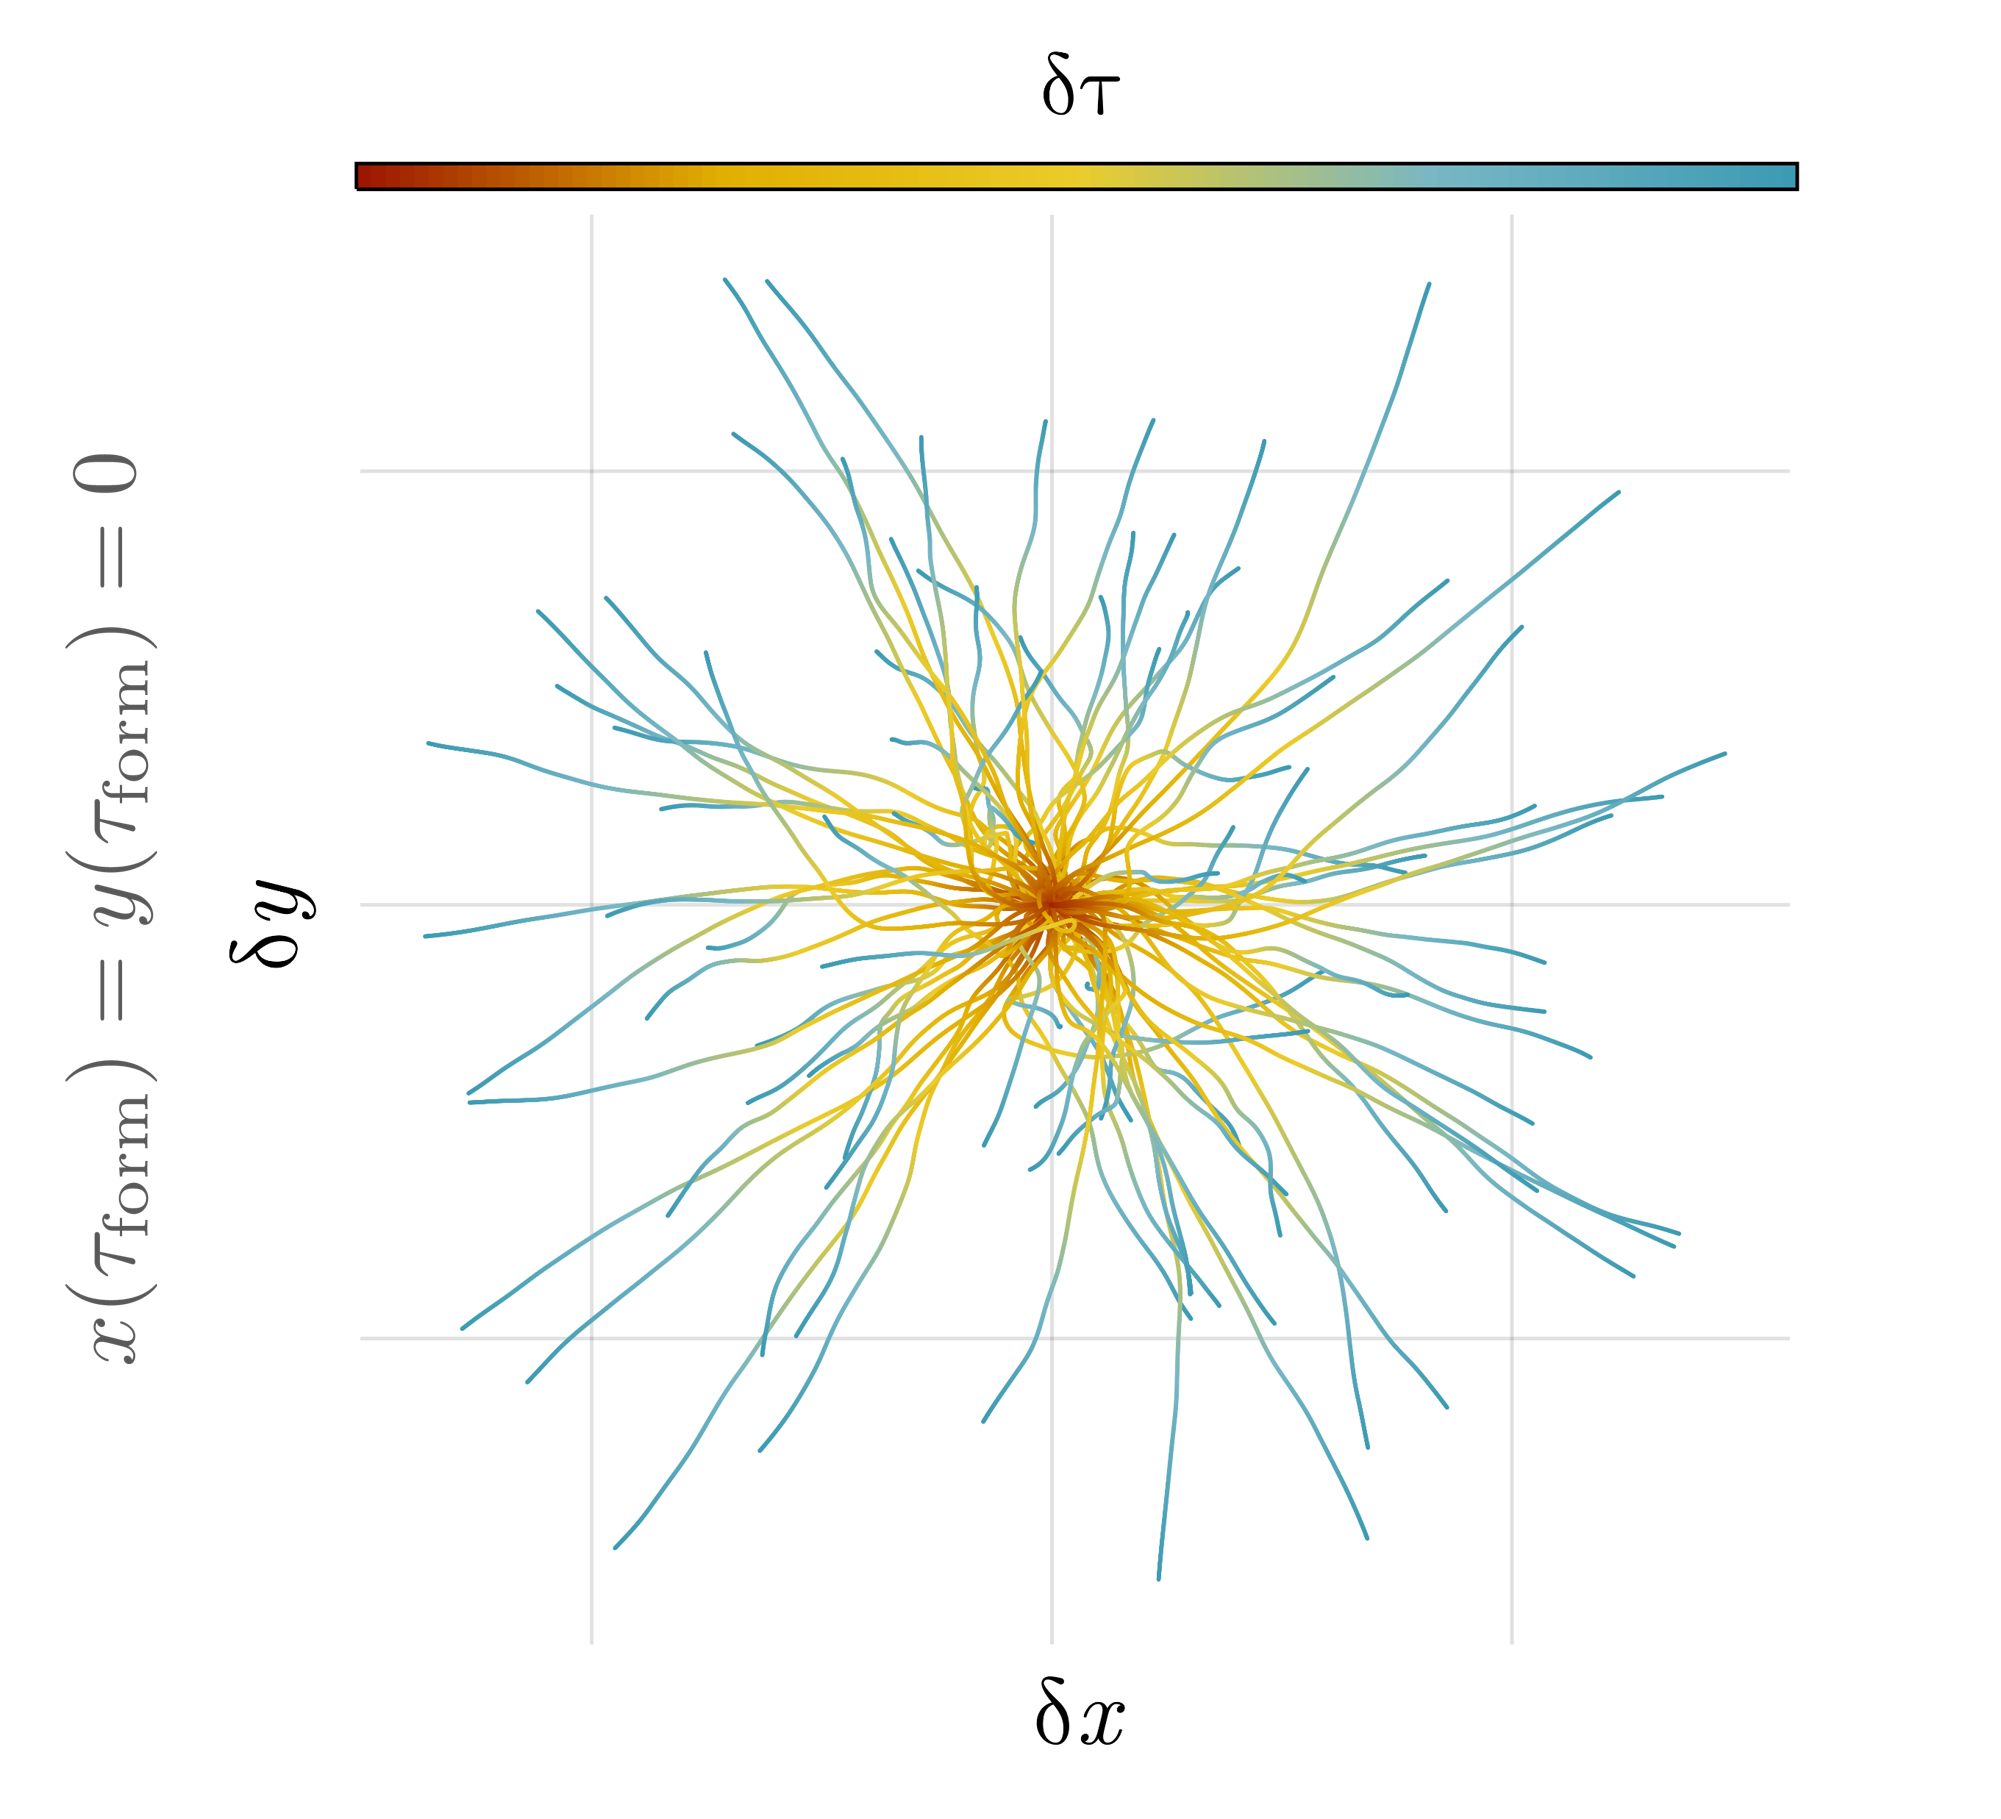
\includegraphics[width=1.1\columnwidth]{images/wong_coord.png}
                \end{figure}
                \column{.025\textwidth}
        \column{.3\textwidth}
            \begin{center}
                Color Lorentz force
            \end{center}
            \vspace{-20pt}
            \begin{figure}[!hbt]
                \centering
                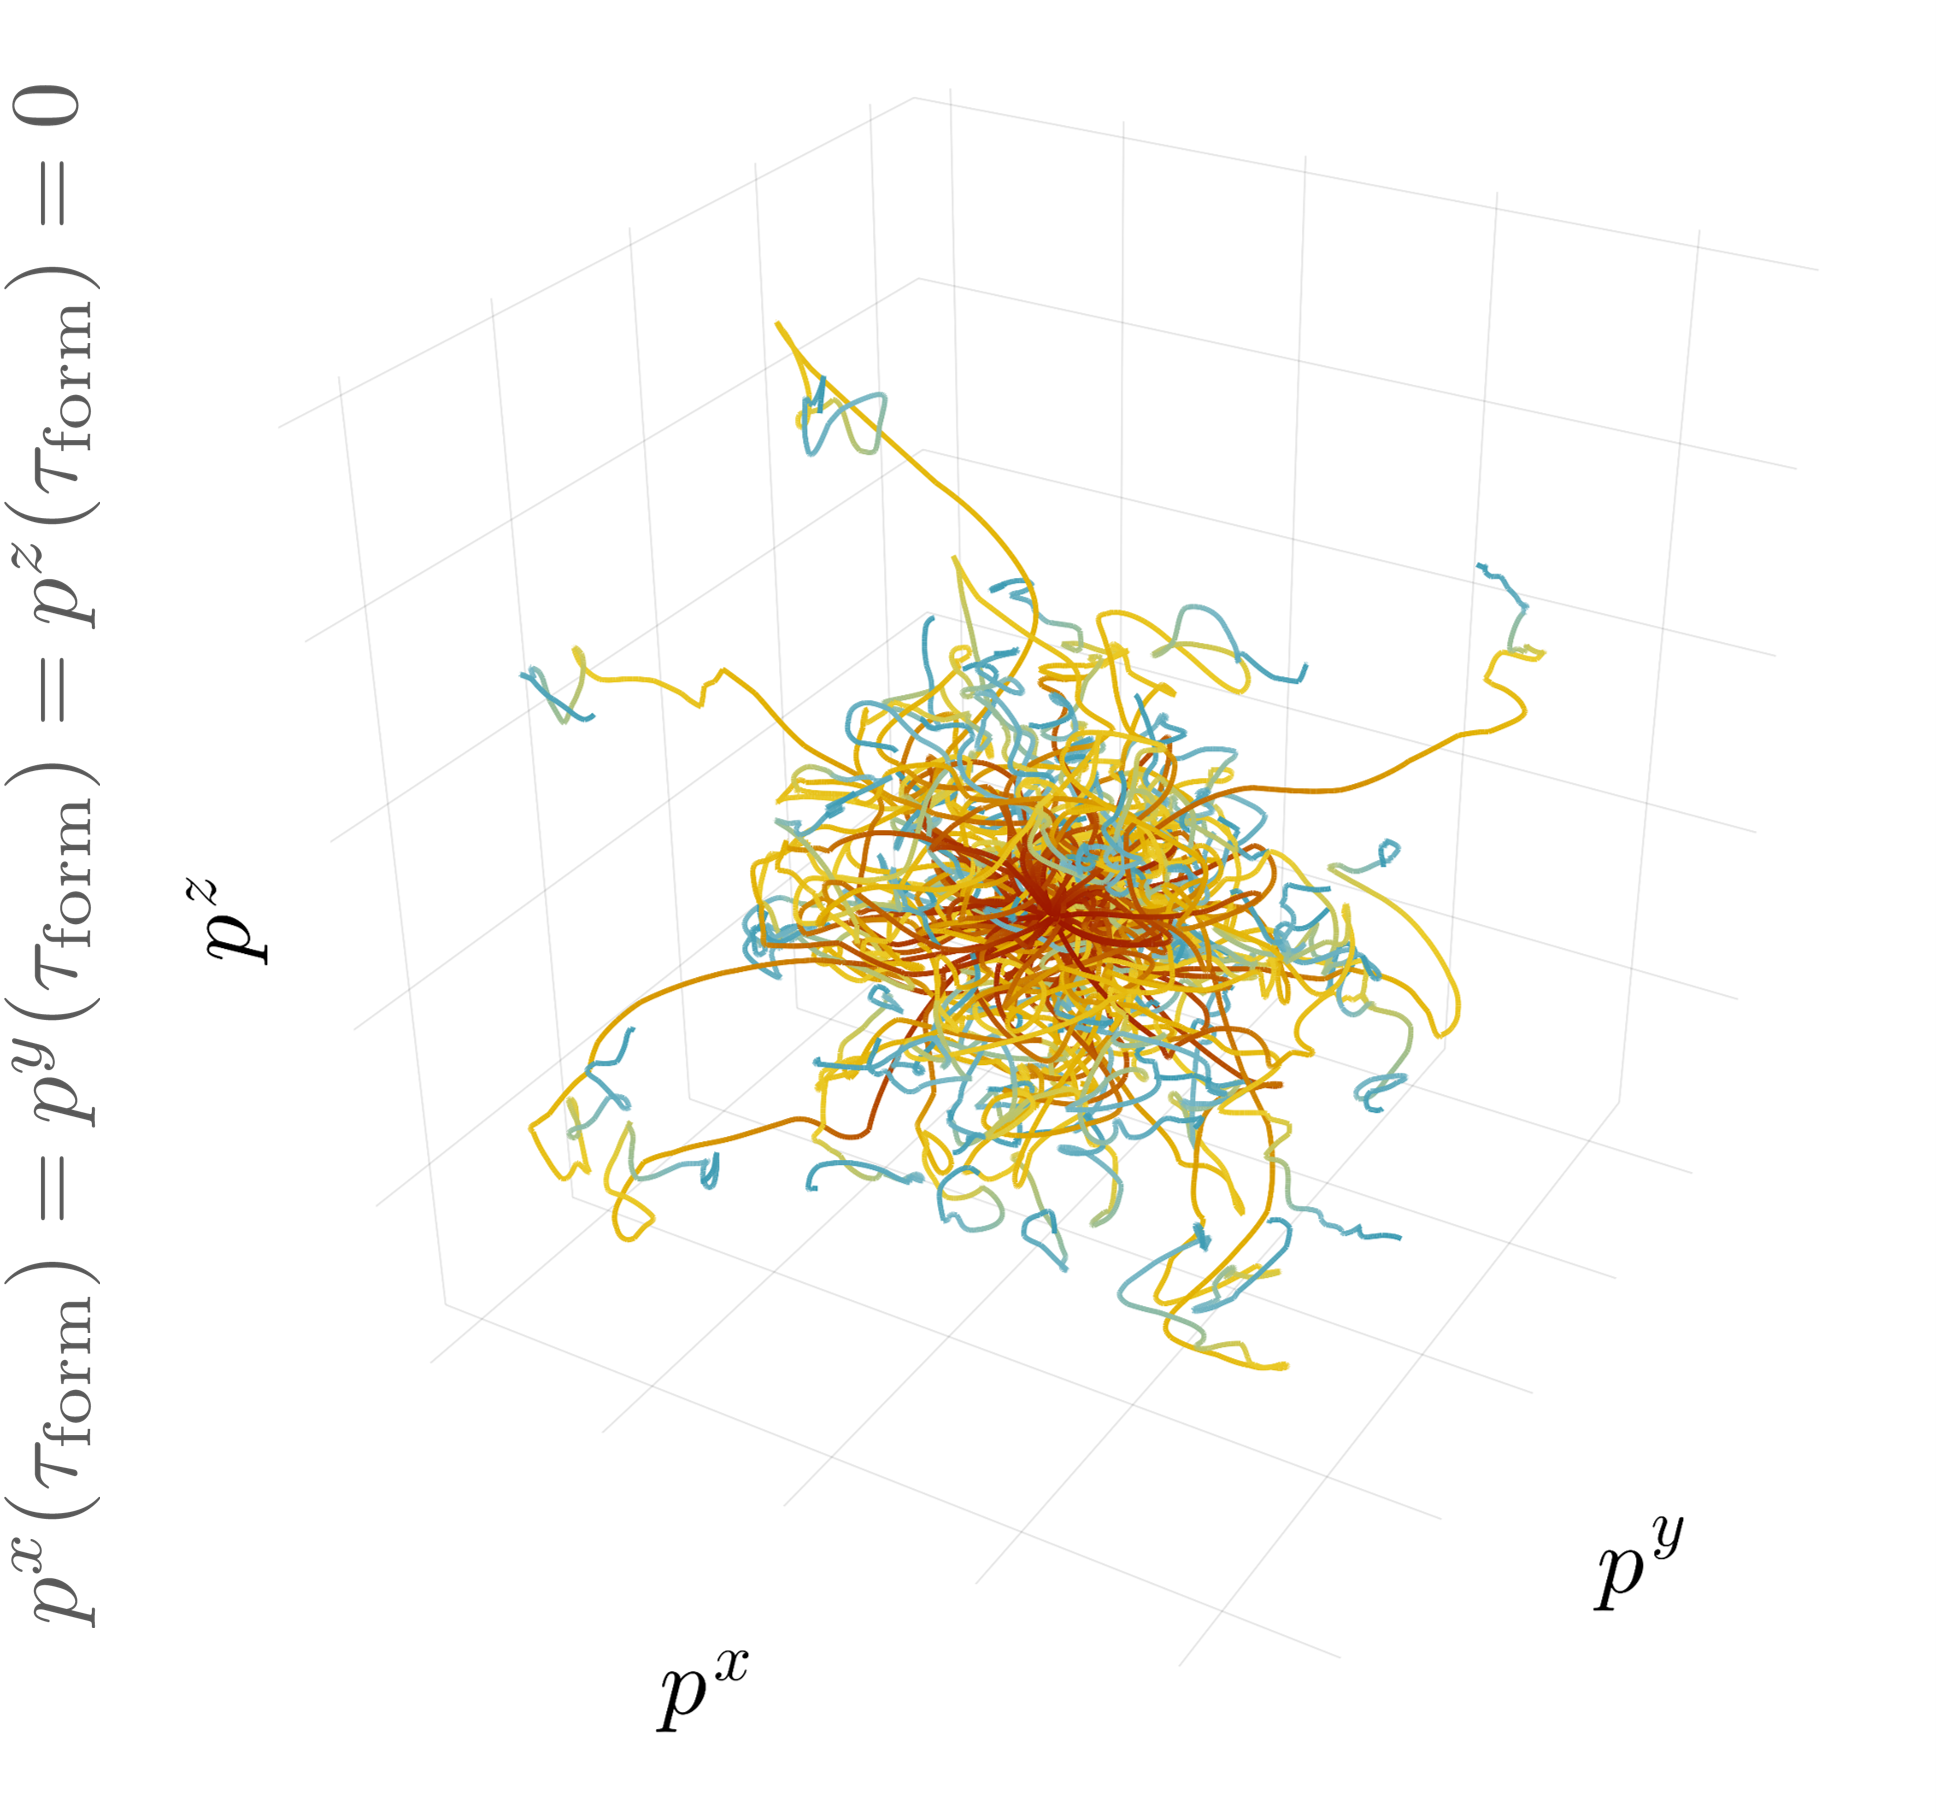
\includegraphics[width=1.1\columnwidth]{images/wong_mom.png}
            \end{figure}
            \column{.025\textwidth}
        \column{.3\textwidth}
            \begin{center}
                Color rotation
            \end{center}
            \vspace{-15pt}
            \begin{figure}[!hbt]
                \centering
                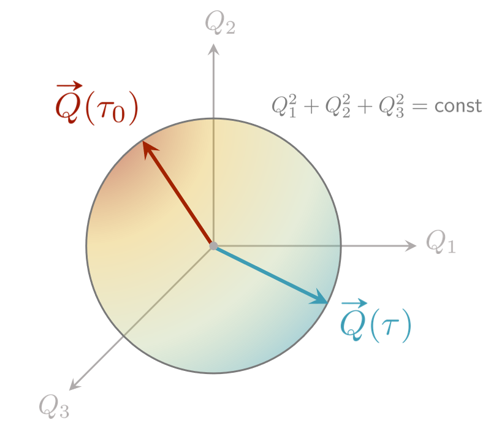
\includegraphics[width=1.05\columnwidth]{images/wong_charge.png}
            \end{figure}
            \column{.025\textwidth}
    \end{columns}
\end{frame}


\begin{frame}[t]
    \frametitle{Timeline}
    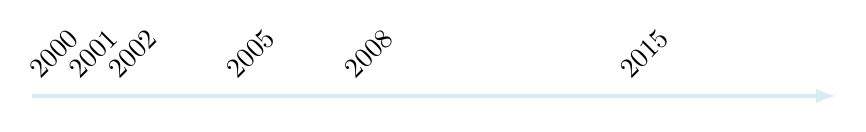
\begin{tikzpicture}[xscale=0.5]%[scale=0.9, every node/.style={scale=0.6}]
    % \draw[line width=2mm,-latex,red!20] (-0.2,0) -- (9,0);
    \draw[line width=0.5mm,-latex,customblue!20] (-0.2,0) -- (20+0.2,0);
    \foreach \X [evaluate=\X as \Y using int(\X-2000),count=\Z] in {2000,2001,2002,2005,2008,2015}
    {
    % \draw[highlight on=<\Z>] ({\Y-0.2},-0.5) -- ({\Y+0.2},-0.5) -- (\Y,-0.1) -- cycle;
    \node[circle, highlight on=<\Z>,inner sep=2pt,color=customblue] at (\Y,0) {};
    \node[anchor=south,highlight on=<\Z>,fill=white,rotate=45,anchor=south
    west,inner sep=0pt] at (\Y,0.2) {\X};
    }
    \end{tikzpicture}
    \begin{itemize}
    \item<1> November 2000: marmots start hibernating
    \end{itemize}
\end{frame}
    
\begin{frame}[t]
    \frametitle{Historial}
    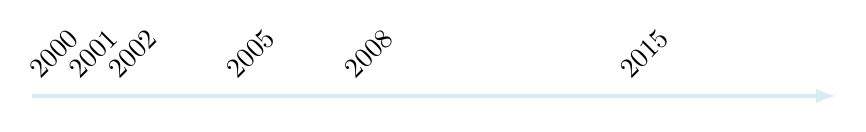
\begin{tikzpicture}[xscale=0.5]
    \draw[line width=0.5mm,-latex,customblue!20] (-0.2,0) -- (20+0.2,0);
    \foreach \X [evaluate=\X as \Y using int(\X-2000),count=\Z] in {2000,2001,2002} %<- these are the years not to be highlighted
    {
    % \draw[highlight on=<0>] ({\Y-0.2},-0.5) -- ({\Y+0.2},-0.5) -- (\Y,-0.1) -- cycle;
    \node[circle, highlight on=<\Z>,inner sep=2pt,color=customblue] at (\Y,0) {};
    \node[anchor=south,highlight on=<0>,fill=white,rotate=45,anchor=south
    west,inner sep=0pt] at (\Y,0.2) {\X};
    }
    \foreach \X [evaluate=\X as \Y using int(\X-2000),count=\Z] in {2005,2008,2015} %<- these are the years which are to be highlighted
    {
    % \draw[highlight on=<\Z>] ({\Y-0.2},-0.5) -- ({\Y+0.2},-0.5) -- (\Y,-0.1) -- cycle;
    \node[circle, highlight on=<\Z>,inner sep=2pt,color=customblue] at (\Y,0) {};
    \node[anchor=south,highlight on=<\Z>,fill=white,rotate=45,anchor=south
    west,inner sep=0pt] at (\Y,0.2) {\X};
    }
    \end{tikzpicture}
    \begin{itemize}
        \item<1> November 2005: marmots start hibernating again
    \end{itemize}
\end{frame}



\subsection{Kinetic theory}
\setbeamertemplate{background}{
\tikz[overlay,remember picture] \node[opacity=0.1, at=(current page.center), align=center] {\\[10pt]
{\transparent{0.2}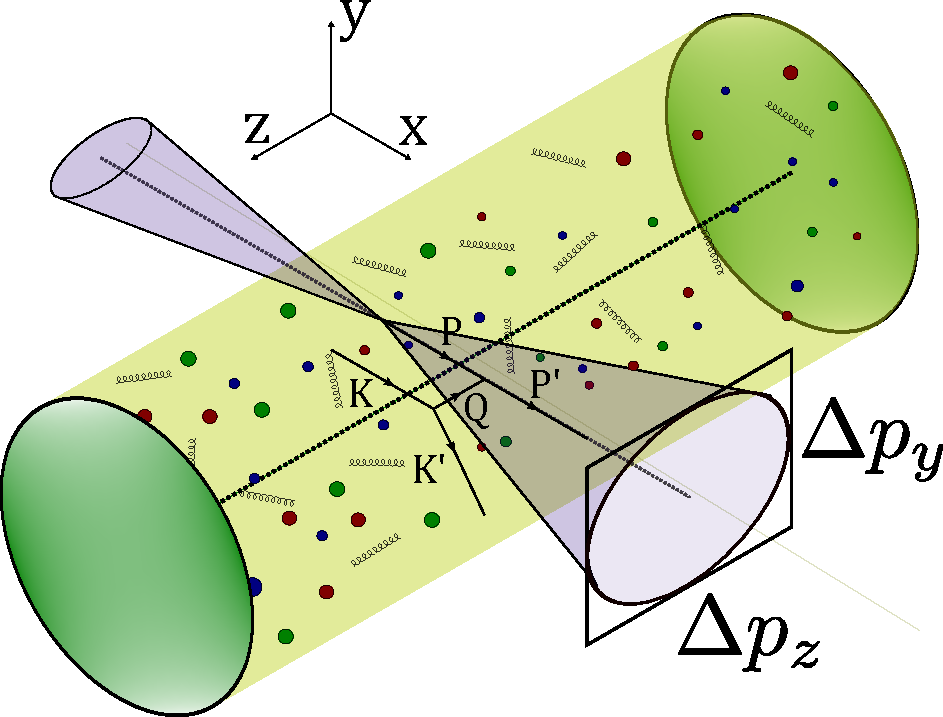
\includegraphics[height=0.7\paperheight]{images/heavy-ion3.pdf}}
   \\[10pt]  
   {\transparent{0.5}\footnotesize\itshape Figure from  K. Boguslavski, A. Kurkela, T. Lappi, F. Lindenbauer, J. Peuron \href{https://arxiv.org/abs/2312.00447}{{\color{lightgray}\texttt{[2312.00447]}}}}};
}
\begin{frame}[plain,noframenumbering]{}
    \begin{center}
        \vspace{1cm}
        {\large\color{normal}Next stages of pre-equilibrium}\\[0.3cm]
        {\huge\color{destacado}Thermalization of heavy quarks}
    \end{center}
\end{frame}
\setbeamertemplate{background}{}


%%%%%%%%%%%%%%%%%%%%%%%%%%%%%%%%%%%%%%%%%%%
%%%%%%%%%%%%%%%% SECTION 4 %%%%%%%%%%%%%%%%
%%%%%%%%%%%%%%%%%%%%%%%%%%%%%%%%%%%%%%%%%%%

\section{Open questions}

\begin{frame}
    \frametitle{Title}
    \framesubtitle{Subtitle}
\end{frame}


% \section{Introduction}
% \subsection{Framework}

% %%%%%%%%%%%%%%%%%%%%%%%%%%%%%%%%%%%%%%%%%%%
% %%%%%%%%%%%%%%%%% SLIDE 1 %%%%%%%%%%%%%%%%%
% %%%%%%%%%%%%%%%%%%%%%%%%%%%%%%%%%%%%%%%%%%%

% \begin{frame}
%     \frametitle{Heavy-ion collisions}
%     \framesubtitle{Stitching together effective theories}
%         % \begin{center}
%         %     Heavy-ion collision $\leftrightarrow$ multi-stage process with each stage $\mapsto$ effective theory
%         % \end{center}
%     \begin{figure}[!hbt]
%         \centering
%     	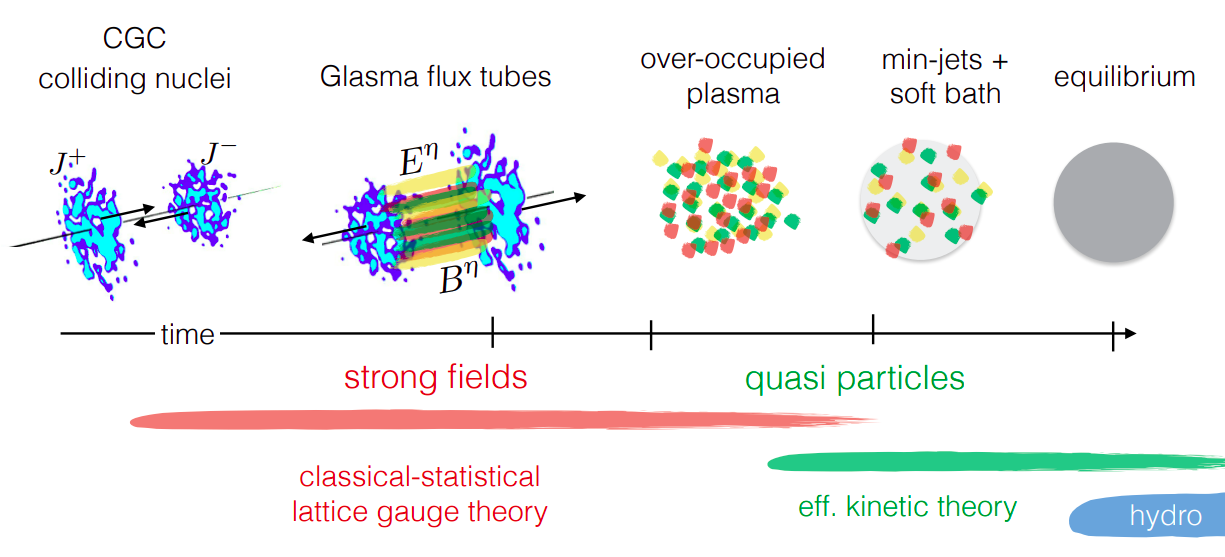
\includegraphics[width=0.8\textwidth]{images/schlichting_initial_stages_2016.png}
%         \captionsetup{justification=centering}
%         % \vspace{-0.6em}
%         \caption{\scriptsize\itshape Figure credits to S. Schlichting}
%     \end{figure}
% \end{frame}

% \begin{frame}[noframenumbering]
%     \frametitle{Heavy-ion collisions}
%     \framesubtitle{Stitching together effective theories}
%         % \begin{center}
%         %     Heavy-ion collision $\leftrightarrow$ multi-stage process with each stage $\mapsto$ effective theory
%         % \end{center}
%     \begin{figure}[!hbt]
%         \centering
%     	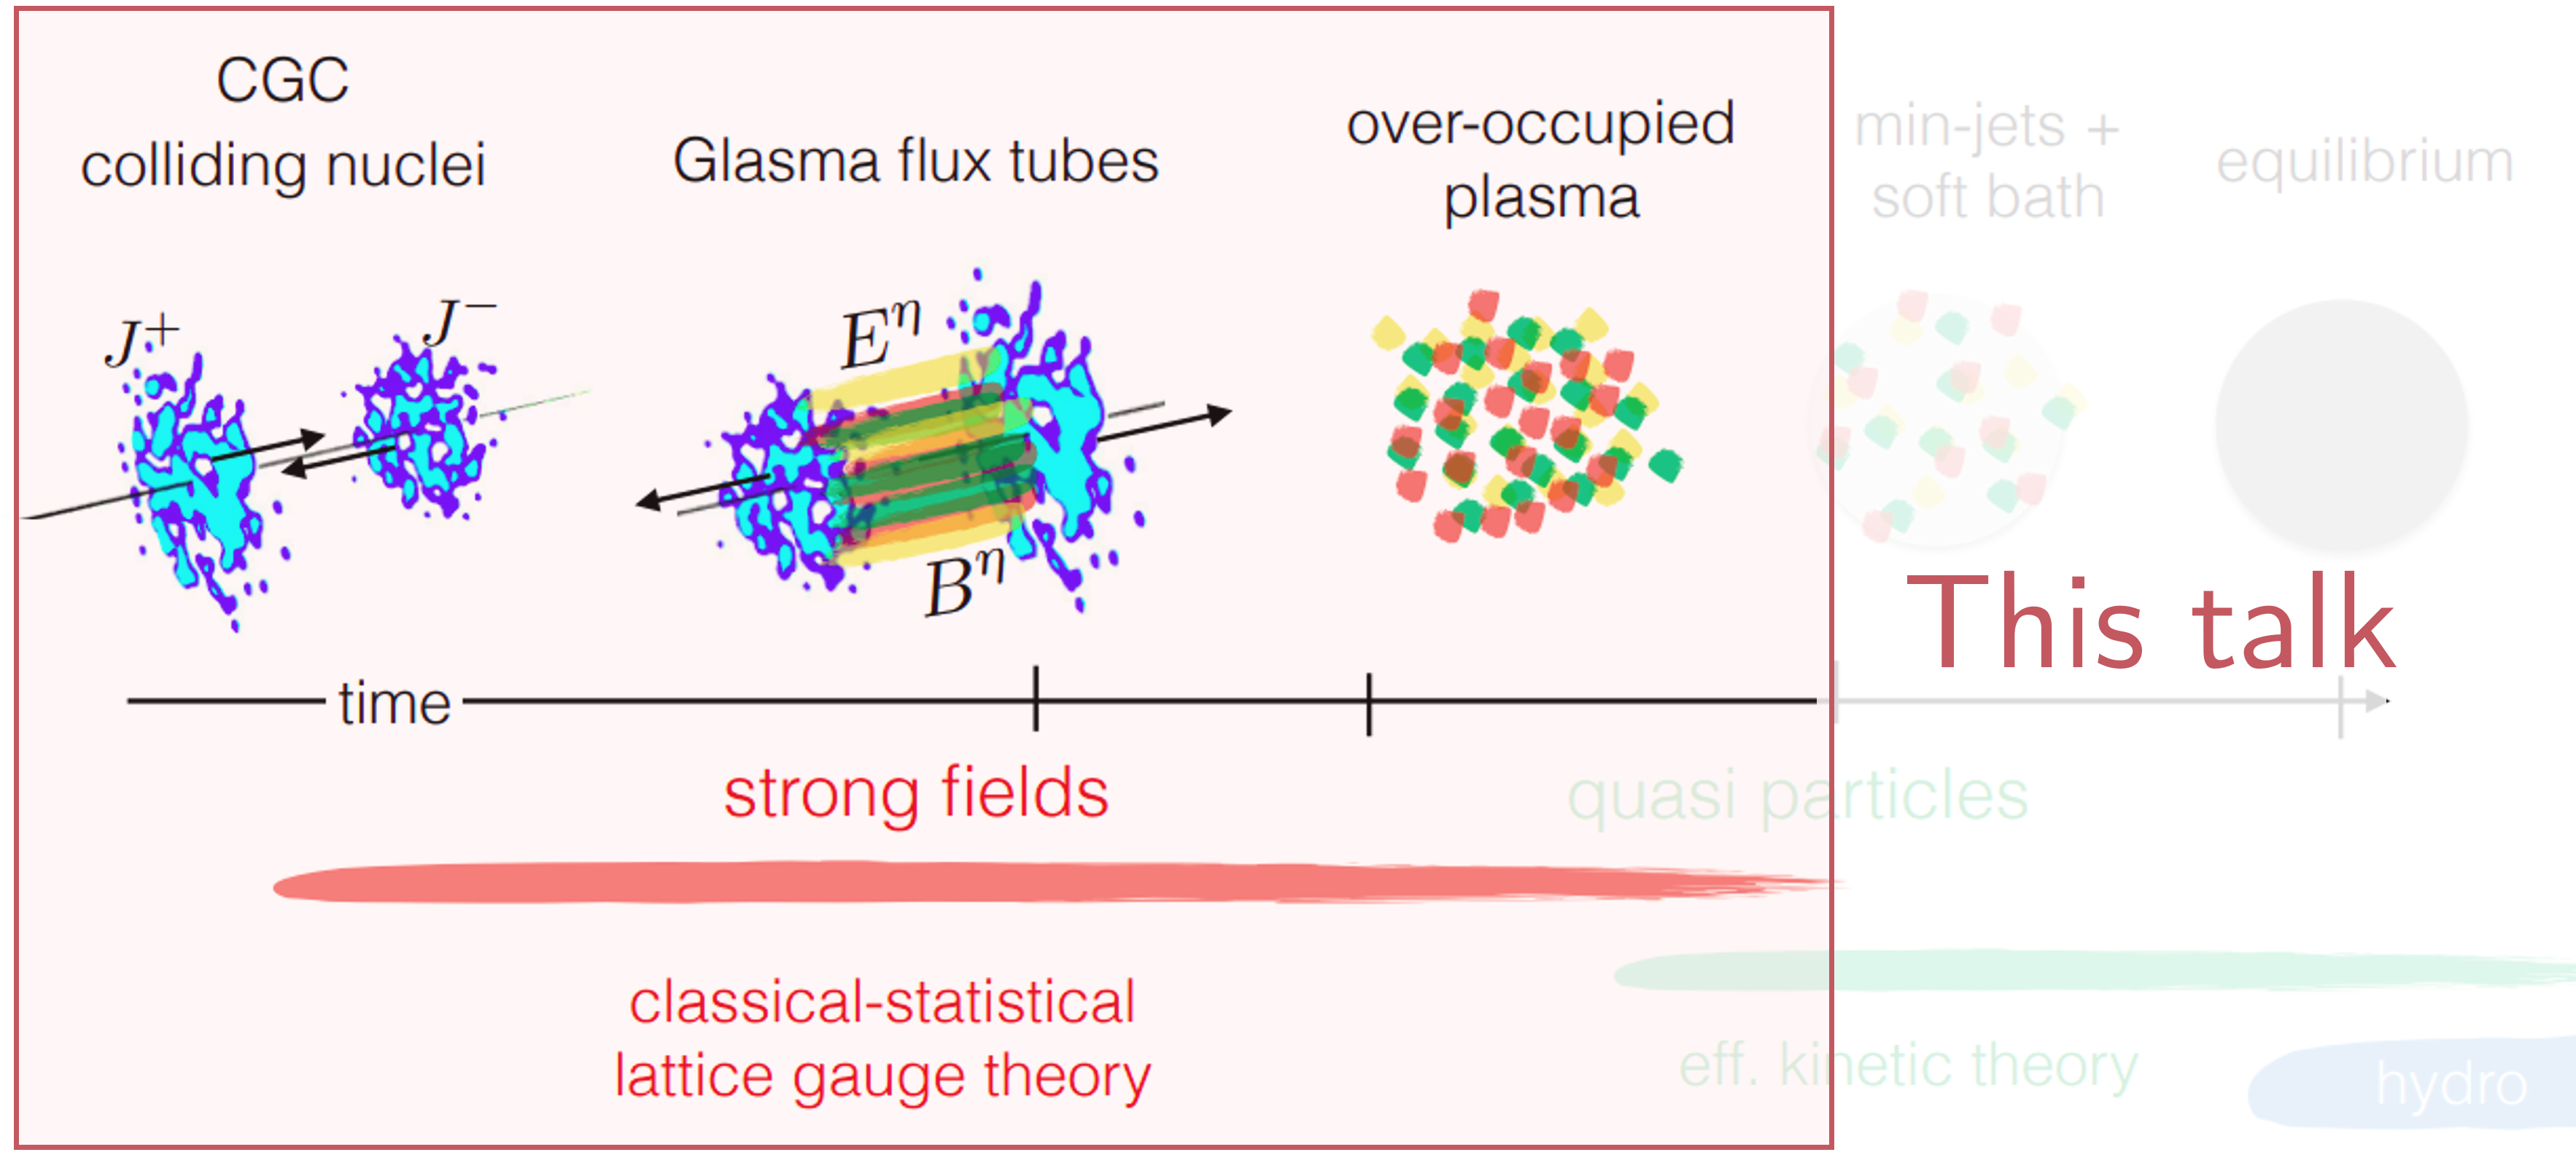
\includegraphics[width=0.8\textwidth]{images/schlichting_initial_stages_2016_thistalk.png}
%         \captionsetup{justification=centering}
%         % \vspace{-0.6em}
%         \caption{\scriptsize\itshape Figure credits to S. Schlichting}
%     \end{figure}
% \end{frame}


% \subsection{Literature}

% %%%%%%%%%%%%%%%%%%%%%%%%%%%%%%%%%%%%%%%%%%%%%
% %%%%%%%%%%%%%%%%% SLIDES 3 %%%%%%%%%%%%%%%%%
% %%%%%%%%%%%%%%%%%%%%%%%%%%%%%%%%%%%%%%%%%%%%%

% % %%%%%%%%%%%%%%%%%%%%%%%%%%%%%%%%%%%%%%%%%%%%%
% % %%%%%%%%%%%%%%%%% SLIDE 3.1 %%%%%%%%%%%%%%%%%
% % %%%%%%%%%%%%%%%%%%%%%%%%%%%%%%%%%%%%%%%%%%%%%

% \begin{frame}
%     \frametitle{Hard probes in the pre-equilibrium stage}
%     \framesubtitle{Literature timeline}
%     \begin{columns}
%     \begin{column}{0.05\textwidth}\end{column}
%     \begin{column}{0.5\textwidth}
%     \footnotesize
%        \begin{tikzpicture}[scale=0.5,every node/.style={outer sep=5pt}]
%         %Notation: {year, the title of the event}
%         %NOTE! Everyting is zero-based
%         \def\ourInfo{{
%             {"2018","Das, Ruggieri 
%             \color{normal}\href{https://arxiv.org/abs/1805.09617}{{\color{lightgray}\textit{[1805.09617]}}}"},
%             {"2020","Ipp \textit{\color{normal}et al.}"},
%             {"2021","Carrington \textit{\color{normal}et al.}"},
%             {"2023","Boguslavski \textit{\color{normal}et al.}"},
%             {"2024","Barata \textit{\color{normal}et al.}"},
%         }}
%         \pgfmathsetmacro{\length}{4}% Zero based.
%         % Loop through the array containing all events.
%         \foreach \i in {0, ..., \length}{
%             \pgfmathsetmacro{\year}{\ourInfo[\i][0]}% Get the left cell (year)
%             \pgfmathsetmacro{\eventName}{\ourInfo[\i][1]}% Get the right cell (event name)
%             \draw[thick,customblue] (0,-2*\i-2)--(0,-2*\i);% Draw vertical line
%             \ifnum \i=0 % Should be in red text
%               \draw(0,-2*\i-1) node[customblue, right, align = left]{\eventName};% Display the event name
%               \draw(0,-2*\i-1) node[customblue, left] {\year};
%             \else % Should be in black text
%                \draw(0,-2*\i-1) node[right, align = left]{\eventName};% Display the event name
%                \draw(0,-2*\i-1) node[left] {\year};% Display the year
%             \fi
%         }
%         % Draw the bullet with the dash
%         \foreach \i in {0, ..., \length}{
%             \filldraw[draw = white, fill = customblue,thick] (0,-2*\i-1) circle (5pt);
%             % \draw[thick,customblue] (-12pt,-2*\i-1)--(0,-2*\i-1);
%         }
%     \end{tikzpicture}
%     \end{column}
%     \begin{column}{0.4\textwidth} 
%         \footnotesize
%         \begin{figure}[!hbt]
%             \centering
%             \captionsetup{justification=centering}
%             \caption{{\large Heavy quarks in Glasma} \\[5pt]
%             {\color{customblue}Highlights}: Diffusion, $R_{pA}$}
%             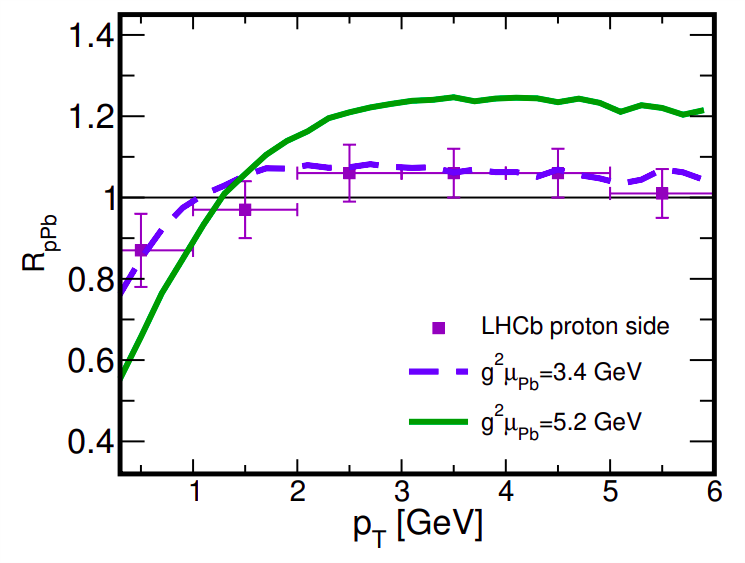
\includegraphics[width=0.85\textwidth]{img/pPb_RpPb_screenshot.png}  
%         \end{figure}
%     \end{column}
%     \begin{column}{0.05\textwidth}\end{column}
%     \end{columns}
% \end{frame}

% % %%%%%%%%%%%%%%%%%%%%%%%%%%%%%%%%%%%%%%%%%%%%%
% % %%%%%%%%%%%%%%%%% SLIDE 3.2 %%%%%%%%%%%%%%%%%
% % %%%%%%%%%%%%%%%%%%%%%%%%%%%%%%%%%%%%%%%%%%%%%

% \addtocounter{framenumber}{-1}
% \begin{frame}
%     \frametitle{Hard probes in the pre-equilibrium stage}
%     \framesubtitle{Literature timeline}
%     \begin{columns}
%     \begin{column}{0.05\textwidth}\end{column}
%     \begin{column}{0.5\textwidth}
%     \footnotesize
%        \begin{tikzpicture}[scale=0.5,every node/.style={outer sep=5pt}]
%         \def\ourInfo{{
%             {"2018","Heavy quarks in Glasma"},
%             {"2020","Ipp, Müller, Schuh
%             \color{normal} \href{https://arxiv.org/abs/2009.14206}{\textit{\color{lightgray}[2009.14206]}}"},
%             {"2021","Carrington \textit{et al.}"},
%             {"2023","Boguslavski \textit{et al.}"},
%             {"2024","Barata \textit{et al.}"},
%         }}
%         \pgfmathsetmacro{\length}{4}
%         \foreach \i in {0, ..., \length}{
%             \pgfmathsetmacro{\year}{\ourInfo[\i][0]}
%             \pgfmathsetmacro{\eventName}{\ourInfo[\i][1]}
%             \draw[thick,customblue] (0,-2*\i-2)--(0,-2*\i);
%             \ifnum \i=1
%               \draw(0,-2*\i-1) node[customblue, right, align = left]{\eventName};
%               \draw(0,-2*\i-1) node[customblue, left] {\year};
%             \else 
%                \draw(0,-2*\i-1) node[right, align = left]{\eventName};
%                \draw(0,-2*\i-1) node[left] {\year};
%             \fi
%         }
%         \foreach \i in {0, ..., \length}{
%             \filldraw[draw = white, fill = customblue,thick] (0,-2*\i-1) circle (5pt);
%         }
%     \end{tikzpicture}
%     \end{column}
%     \begin{column}{0.4\textwidth} 
%         \footnotesize
%     \begin{figure}[!hbt]
%             \centering
%             \captionsetup{justification=centering}
%             \caption{{\large Eikonal jets in Glasma} \\[5pt] {\color{customblue}Highlights}: Lattice simulations\\ Transport coefficient $\hat{q}$}
%             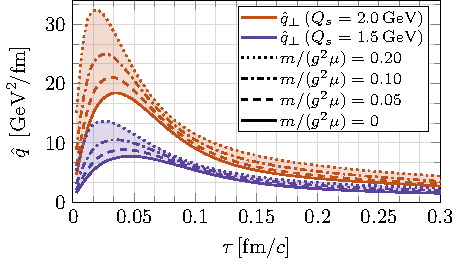
\includegraphics[width=0.9\textwidth]{img/qhat_tau.pdf}
%         \end{figure}
%     \end{column}
%     \begin{column}{0.05\textwidth}\end{column}
%     \end{columns}
% \end{frame}

% % %%%%%%%%%%%%%%%%%%%%%%%%%%%%%%%%%%%%%%%%%%%%%
% % %%%%%%%%%%%%%%%%% SLIDE 3.3 %%%%%%%%%%%%%%%%%
% % %%%%%%%%%%%%%%%%%%%%%%%%%%%%%%%%%%%%%%%%%%%%%

% \addtocounter{framenumber}{-1}
% \begin{frame}
%     \frametitle{Hard probes in the pre-equilibrium stage}
%     \framesubtitle{Literature timeline}
%     \begin{columns}
%     \begin{column}{0.05\textwidth}\end{column}
%     \begin{column}{0.5\textwidth}
%     \footnotesize
%        \begin{tikzpicture}[scale=0.5,every node/.style={outer sep=5pt}]
%         \def\ourInfo{{
%             {"2018","Heavy quarks in Glasma"},
%             {"2020","Eikonal jets in Glasma"},
%             {"2021","Carrington, Czajka, Mrowczynski \\
%             \color{normal} \href{https://arxiv.org/abs/2202.00357}{\textit{\color{lightgray}[2202.00357]}}"},
%             {"2023","Boguslavski \textit{et al.}"},
%             {"2024","Barata \textit{et al.}"},
%         }}
%         \pgfmathsetmacro{\length}{4}
%         \foreach \i in {0, ..., \length}{
%             \pgfmathsetmacro{\year}{\ourInfo[\i][0]}
%             \pgfmathsetmacro{\eventName}{\ourInfo[\i][1]}
%             \draw[thick,customblue] (0,-2*\i-2)--(0,-2*\i);
%             \ifnum \i=2
%               \draw(0,-2*\i-1) node[customblue, right, align = left]{\eventName};
%               \draw(0,-2*\i-1) node[customblue, left] {\year};
%             \else 
%                \draw(0,-2*\i-1) node[right, align = left]{\eventName};
%                \draw(0,-2*\i-1) node[left] {\year};
%             \fi
%         }
%         \foreach \i in {0, ..., \length}{
%             \filldraw[draw = white, fill = customblue,thick] (0,-2*\i-1) circle (5pt);
%         }
%     \end{tikzpicture}
%     \end{column}
%     \begin{column}{0.4\textwidth} 
%         \footnotesize
%     \begin{figure}[!hbt]
%             \centering
%             \captionsetup{justification=centering}
%             \caption{{\large Hard probes in Glasma} \\[5pt]
%             {\color{customblue}Highlight}: Analytical calculations\\
%             Transport coefficient $\hat{q}$}
%             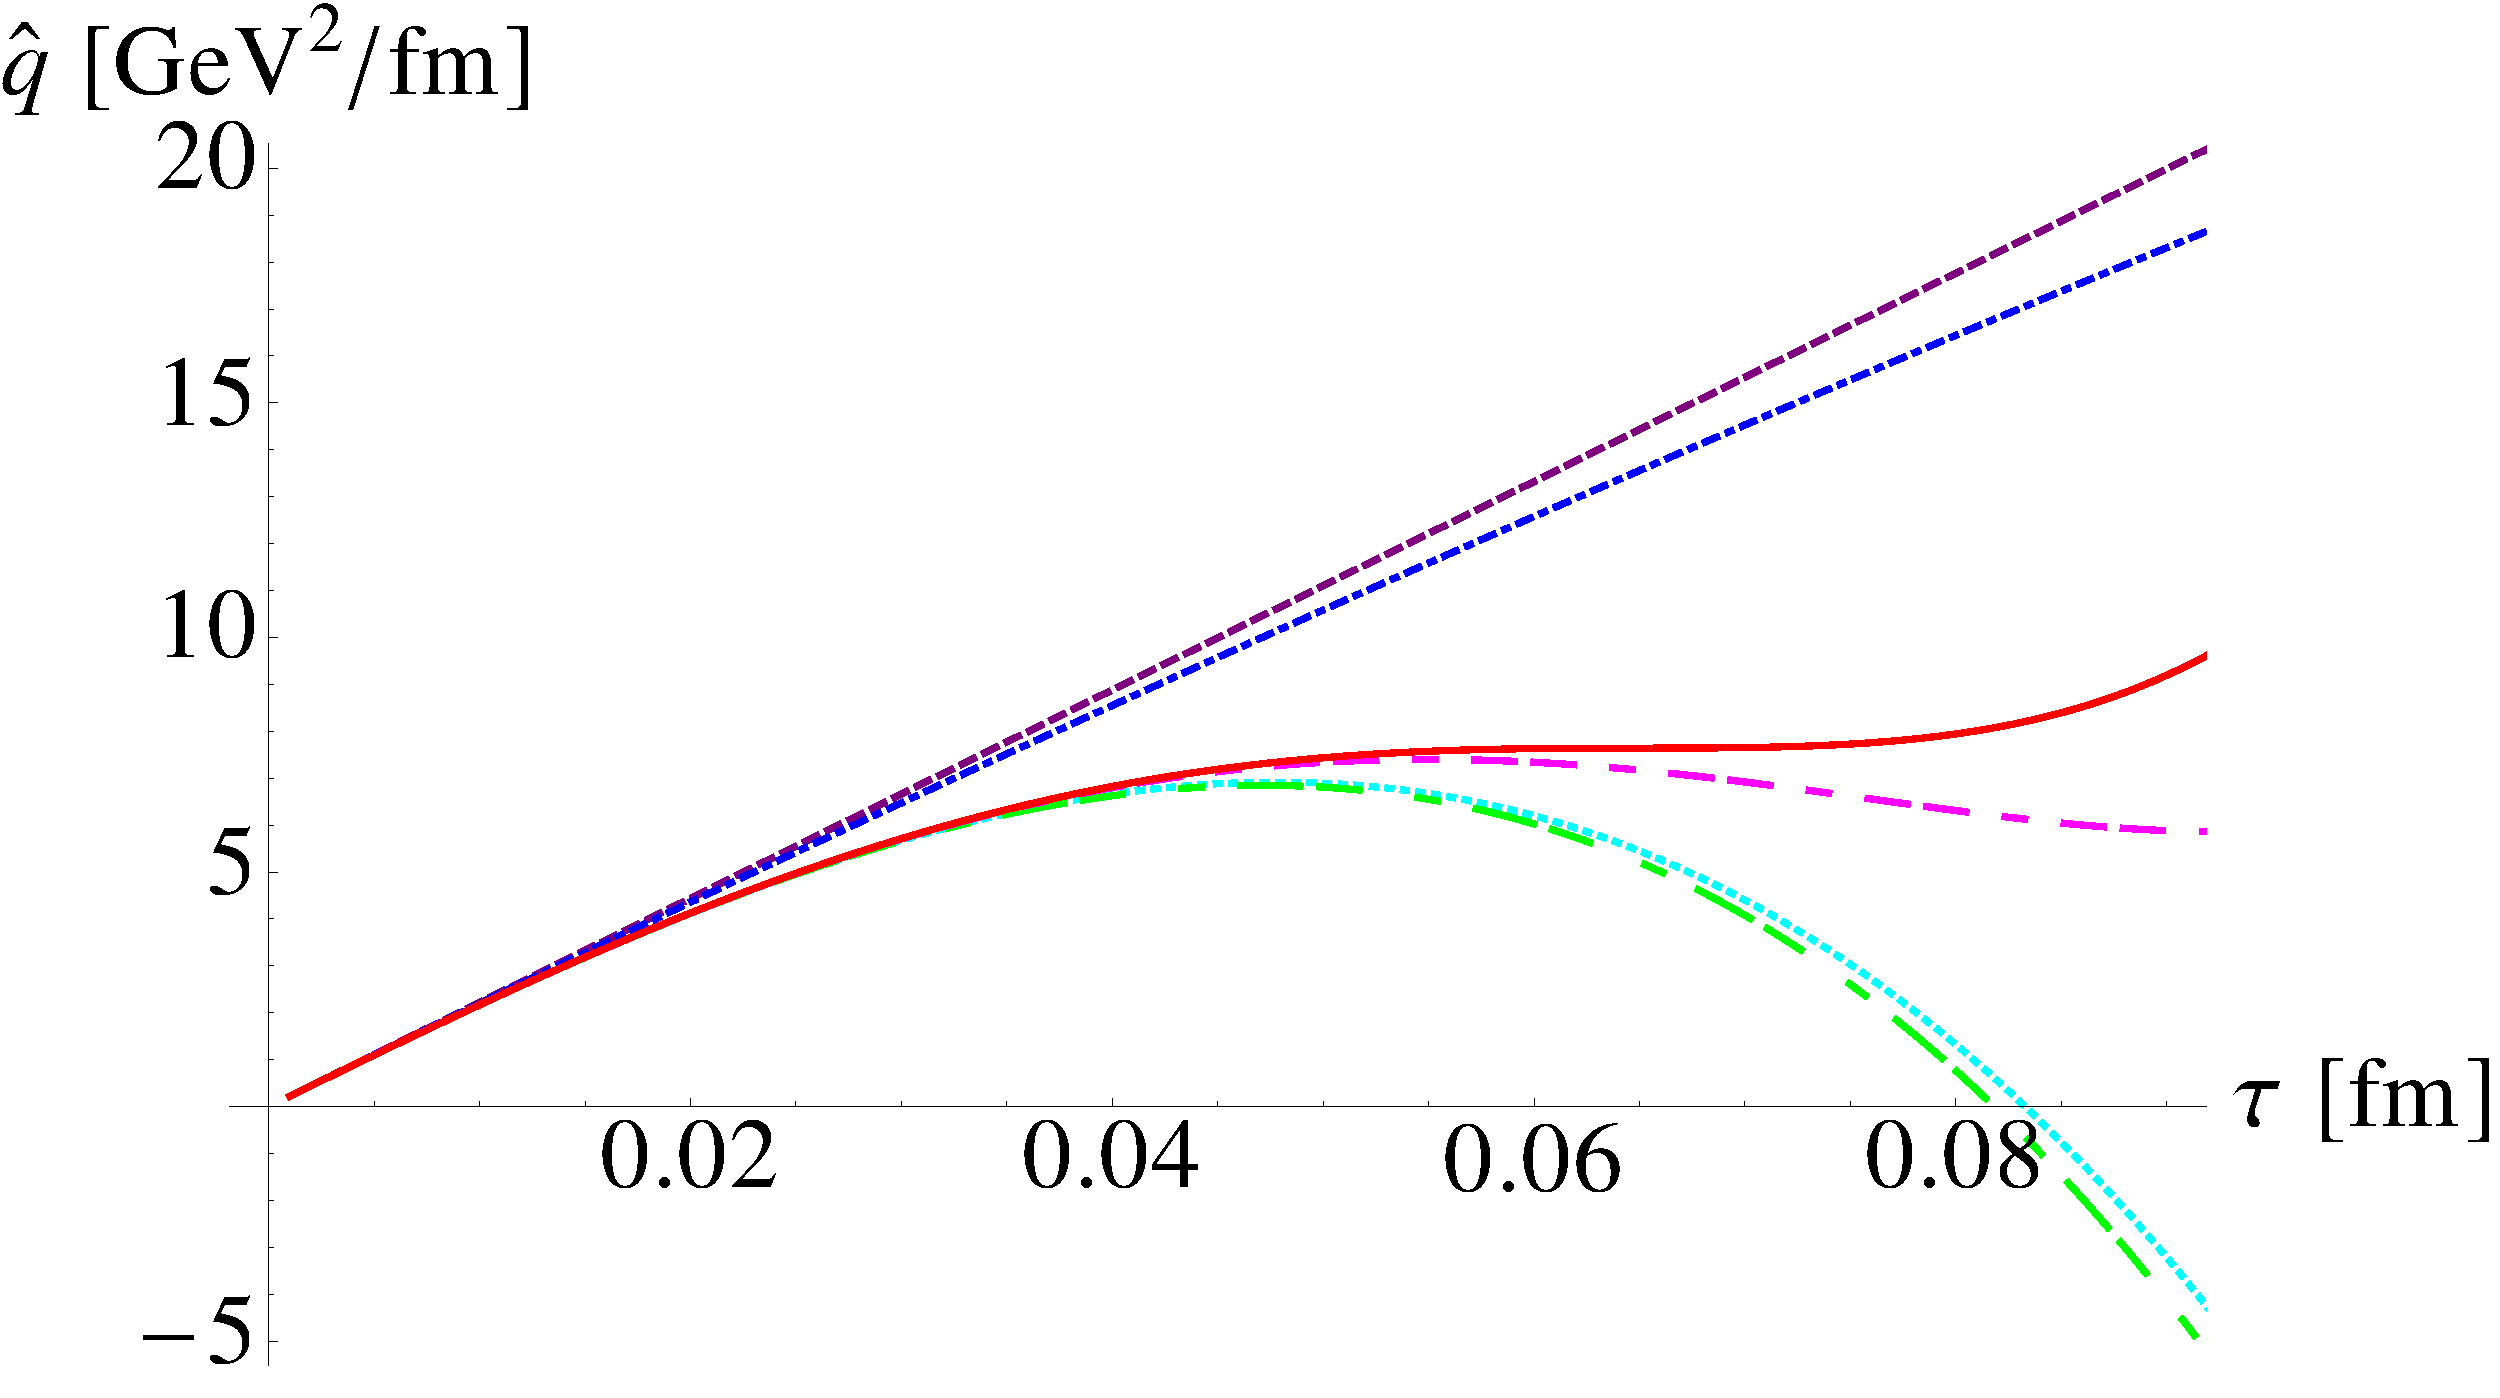
\includegraphics[width=0.85\textwidth]{img/plot-qhat-six-cases.pdf}
%         \end{figure}
%     \end{column}
%     \begin{column}{0.05\textwidth}\end{column}
%     \end{columns}
% \end{frame}

% % %%%%%%%%%%%%%%%%%%%%%%%%%%%%%%%%%%%%%%%%%%%%%
% % %%%%%%%%%%%%%%%%% SLIDE 3.4 %%%%%%%%%%%%%%%%%
% % %%%%%%%%%%%%%%%%%%%%%%%%%%%%%%%%%%%%%%%%%%%%%

% \addtocounter{framenumber}{-1}
% \begin{frame}
%     \frametitle{Hard probes in the pre-equilibrium stage}
%     \framesubtitle{Literature timeline}
%     \begin{columns}
%     \begin{column}{0.05\textwidth}\end{column}
%     \begin{column}{0.5\textwidth}
%     \footnotesize
%        \begin{tikzpicture}[scale=0.5,every node/.style={outer sep=5pt}]
%         \def\ourInfo{{
%             {"2018","Heavy quarks in Glasma"},
%             {"2020","Eikonal jets in Glasma"},
%             {"2021","Hard probes in Glasma"},
%             {"2023","Boguslavski, Kurkela, Lappi, Lindenbauer, Peuron \\ \href{https://arxiv.org/abs/2303.12595}{\color{lightgray}\textit{[2303.12595]}}"},
%             {"2024","Barata \textit{et al.}"},
%         }}
%         \pgfmathsetmacro{\length}{4}
%         \foreach \i in {0, ..., \length}{
%             \pgfmathsetmacro{\year}{\ourInfo[\i][0]}
%             \pgfmathsetmacro{\eventName}{\ourInfo[\i][1]}
%             \draw[thick,customblue] (0,-2*\i-2)--(0,-2*\i);
%             \ifnum \i=3
%               \draw(0,-2*\i-1) node[customblue, right, align = left]{\eventName};
%               \draw(0,-2*\i-1) node[customblue, left] {\year};
%             \else 
%                \draw(0,-2*\i-1) node[right, align = left]{\eventName};
%                \draw(0,-2*\i-1) node[left] {\year};
%             \fi
%         }
%         \foreach \i in {0, ..., \length}{
%             \filldraw[draw = white, fill = customblue,thick] (0,-2*\i-1) circle (5pt);
%         }
%     \end{tikzpicture}
%     \end{column}
%     \begin{column}{0.4\textwidth} 
%     \begin{figure}[!hbt]
%             \centering
%             \captionsetup{justification=centering}
%             \caption{{\large Hard probes in kinetic theory} \\[5pt]
%             {\color{customblue}Highlight}: Stage after Glasma\\
%             Compatible $\hat{q}$ and $\kappa$}
%             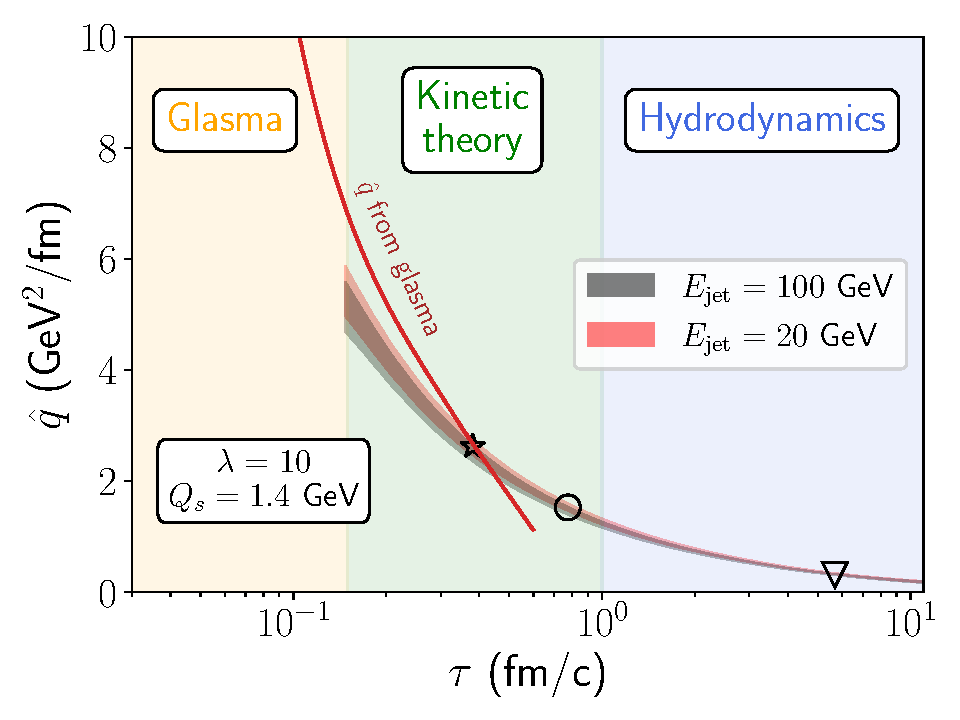
\includegraphics[width=0.8\textwidth]{img/2023-03-07-16-41-35_qhat_appetizer_glasma_comparison_493.pdf}
%         \end{figure}
%     \end{column}
%     \begin{column}{0.05\textwidth}\end{column}
%     \end{columns}
% \end{frame}


% % %%%%%%%%%%%%%%%%%%%%%%%%%%%%%%%%%%%%%%%%%%%%%
% % %%%%%%%%%%%%%%%%% SLIDE 3.5 %%%%%%%%%%%%%%%%%
% % %%%%%%%%%%%%%%%%%%%%%%%%%%%%%%%%%%%%%%%%%%%%%

% \addtocounter{framenumber}{-1}
% \begin{frame}
%     \frametitle{Hard probes in the pre-equilibrium stage}
%     \framesubtitle{Literature timeline}
%     \begin{columns}
%     \begin{column}{0.05\textwidth}\end{column}
%     \begin{column}{0.5\textwidth}
%     \footnotesize
%        \begin{tikzpicture}[scale=0.5,every node/.style={outer sep=5pt}]
%         \def\ourInfo{{
%             {"2018","Heavy quarks in Glasma"},
%             {"2020","Eikonal jets in Glasma"},
%             {"2021","Hard probes in Glasma"},
%             {"2023","Hard probes in kinetic theory"},
%             {"2024","Barata, Hauksson, López, Sadofyev \href{https://arxiv.org/abs/2406.07615}{\color{lightgray}\textit{[2406.07615]}}"},
%         }}
%         \pgfmathsetmacro{\length}{4}
%         \foreach \i in {0, ..., \length}{
%             \pgfmathsetmacro{\year}{\ourInfo[\i][0]}
%             \pgfmathsetmacro{\eventName}{\ourInfo[\i][1]}
%             \draw[thick,customblue] (0,-2*\i-2)--(0,-2*\i);
%             \ifnum \i=4
%               \draw(0,-2*\i-1) node[customblue, right, align = left]{\eventName};
%               \draw(0,-2*\i-1) node[customblue, left] {\year};
%             \else 
%                \draw(0,-2*\i-1) node[right, align = left]{\eventName};
%                \draw(0,-2*\i-1) node[left] {\year};
%             \fi
%         }
%         \foreach \i in {0, ..., \length}{
%             \filldraw[draw = white, fill = customblue,thick] (0,-2*\i-1) circle (5pt);
%         }
%     \end{tikzpicture}
%     \end{column}
%     \begin{column}{0.4\textwidth} 
%     \begin{figure}[!hbt]
%             \centering
%             \captionsetup{justification=centering}
%             \caption{{\large Energy loss in Glasma} \\[5pt]
%             {\color{customblue}Highlight}: Analytical calculations\\
%            Medium-induced gluon radiation}
%             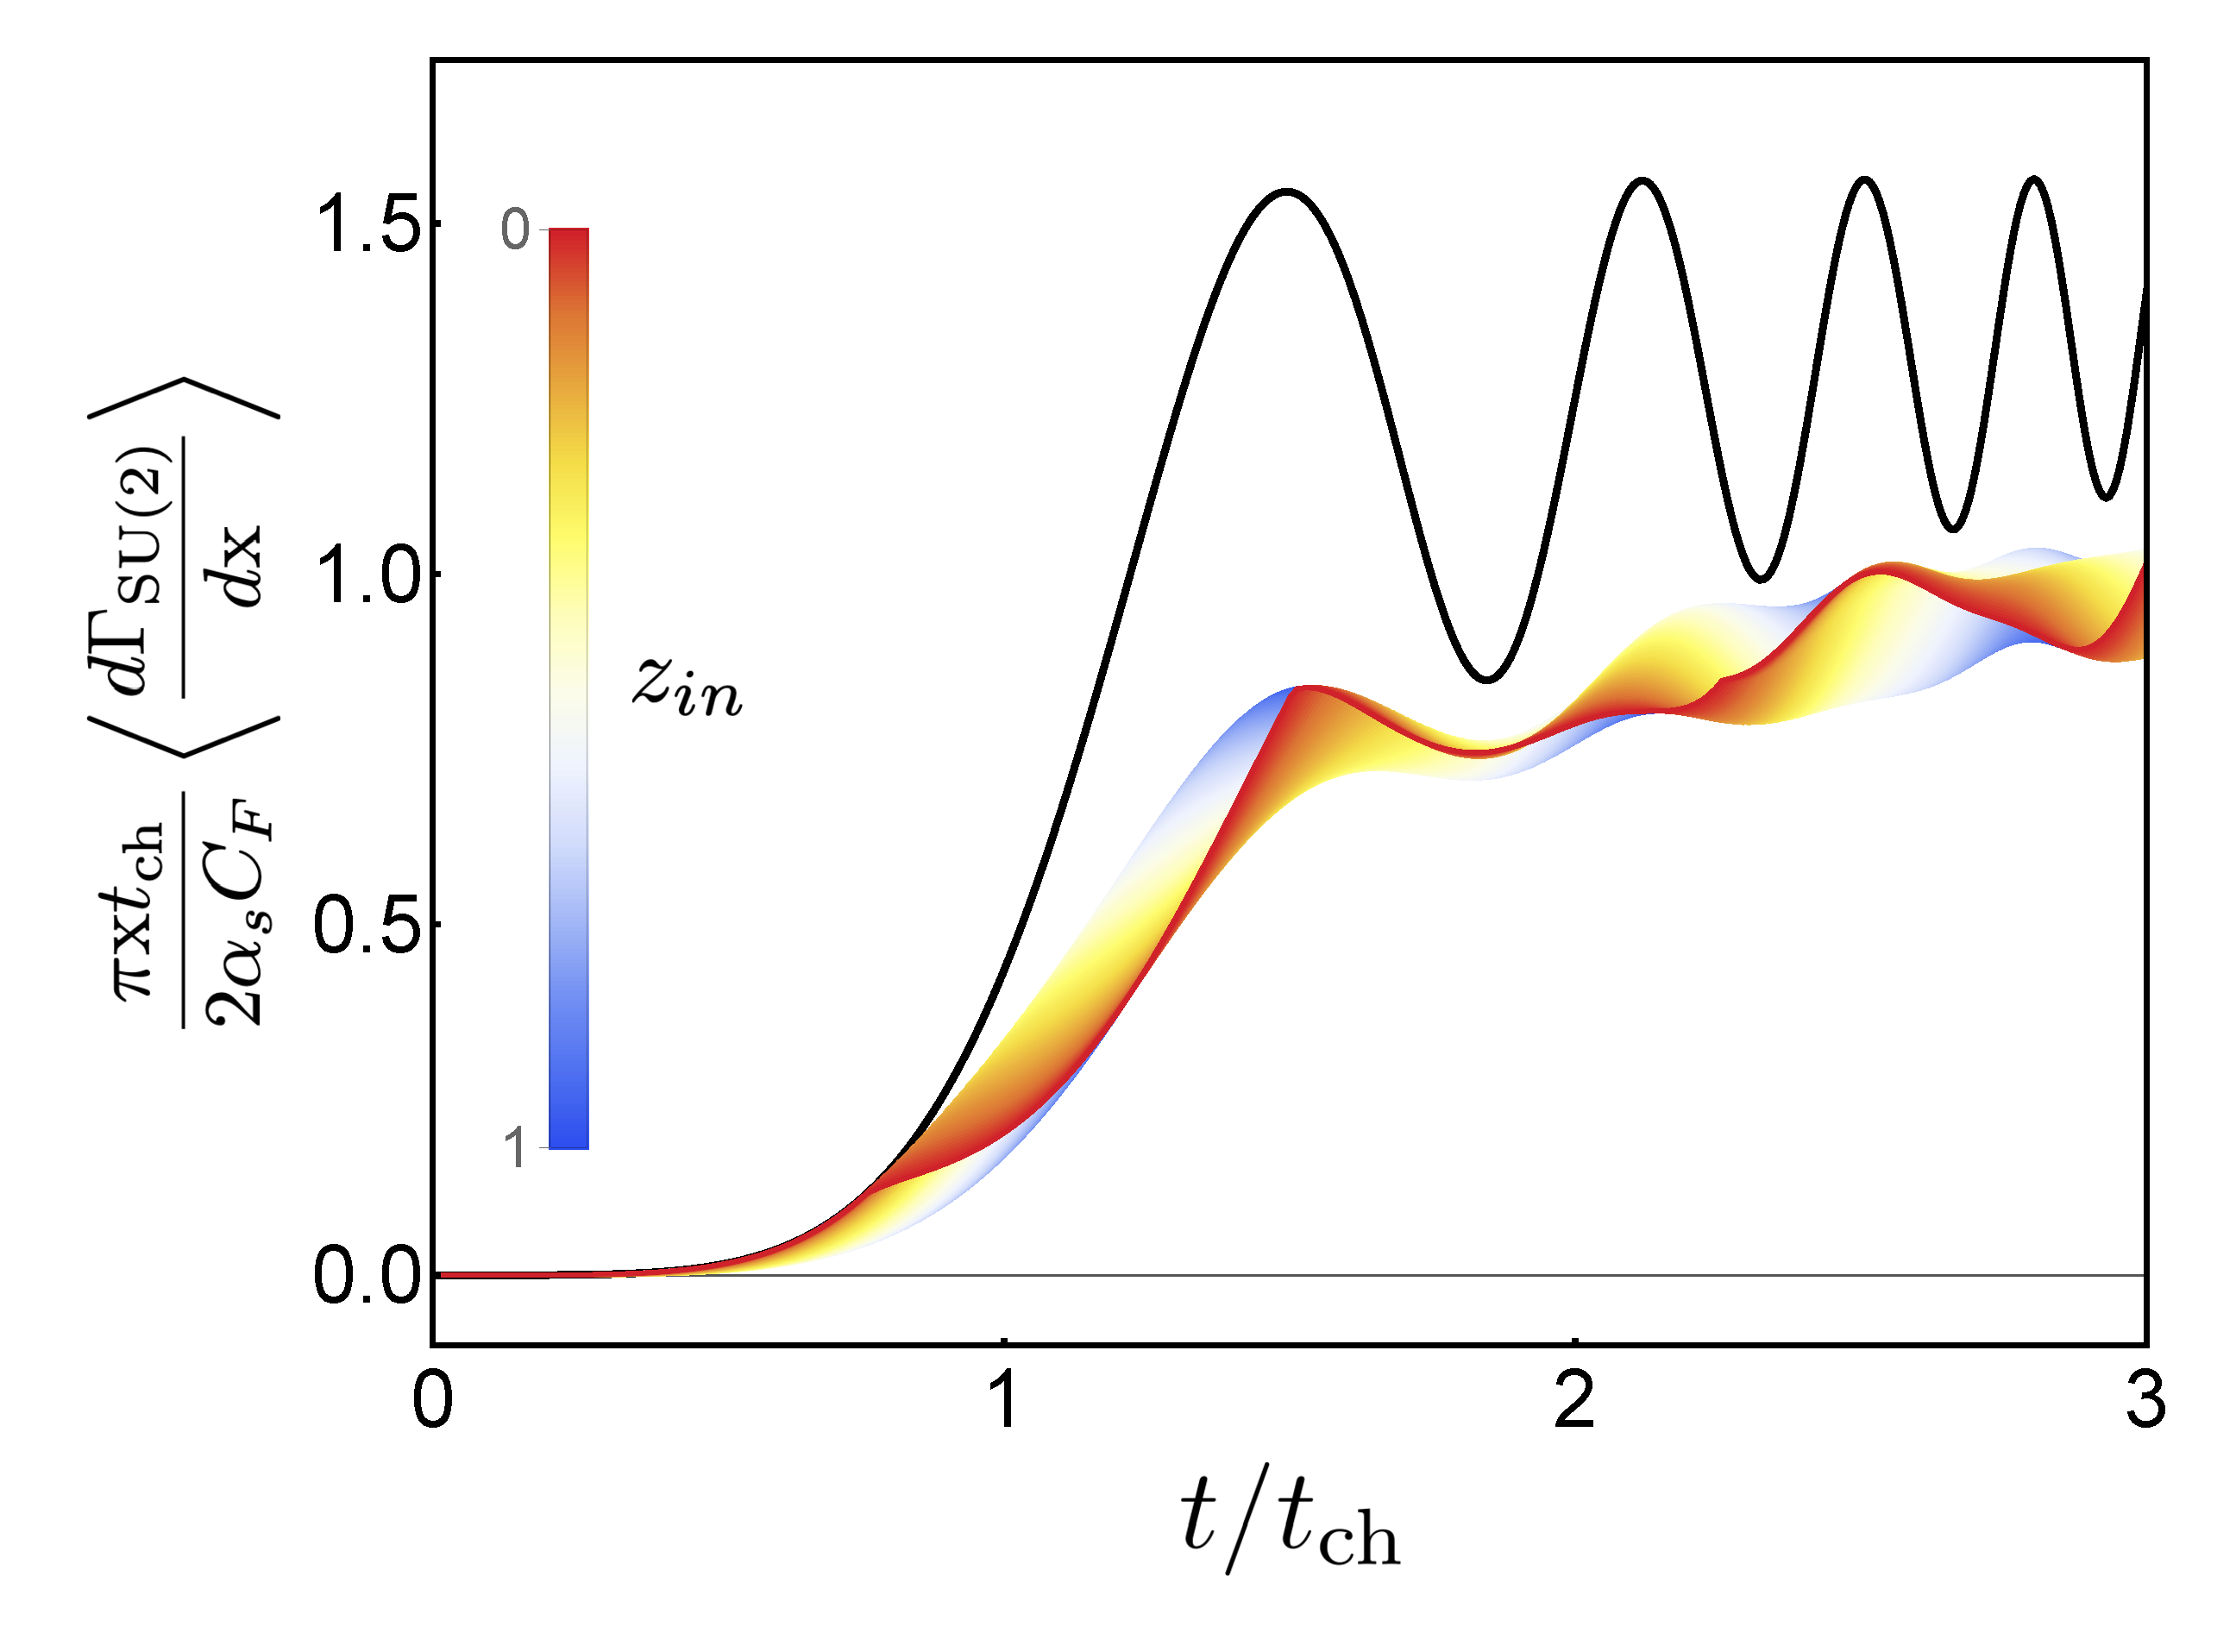
\includegraphics[width=0.8\textwidth]{images/SU2manyallother-cropped.pdf}
%         \end{figure}
%     \end{column}
%     \begin{column}{0.05\textwidth}\end{column}
%     \end{columns}
% \end{frame}


% \subsection{This study}

% %%%%%%%%%%%%%%%%%%%%%%%%%%%%%%%%%%%%%%%%%%%
% %%%%%%%%%%%%%%%%% SLIDE 3 %%%%%%%%%%%%%%%%%
% %%%%%%%%%%%%%%%%%%%%%%%%%%%%%%%%%%%%%%%%%%%


% \begin{frame}
%     \frametitle{Hard probes in Glasma}
%     \framesubtitle{Classical transport in the very-early stage}
%     \begin{center}
%         \onslide<1,2>{\textit{Prerequisite: }{\color{pinky}Classical lattice gauge theory} $\xrightarrow{\text{solver}}$ {\color{customblue}Glasma fields}\\[0.3cm]}\onslide<2>{\textit{This work: }{\color{customblue}Glasma fields} $\xleftrightarrow{\text{background}}$ test {\color{customgreen}particles} $\xleftarrow{\text{solver}}$ {\color{pinky}colored particle-in-cell}}
%         \begin{figure}[!hbt]
%             \centering
%             \only<1>{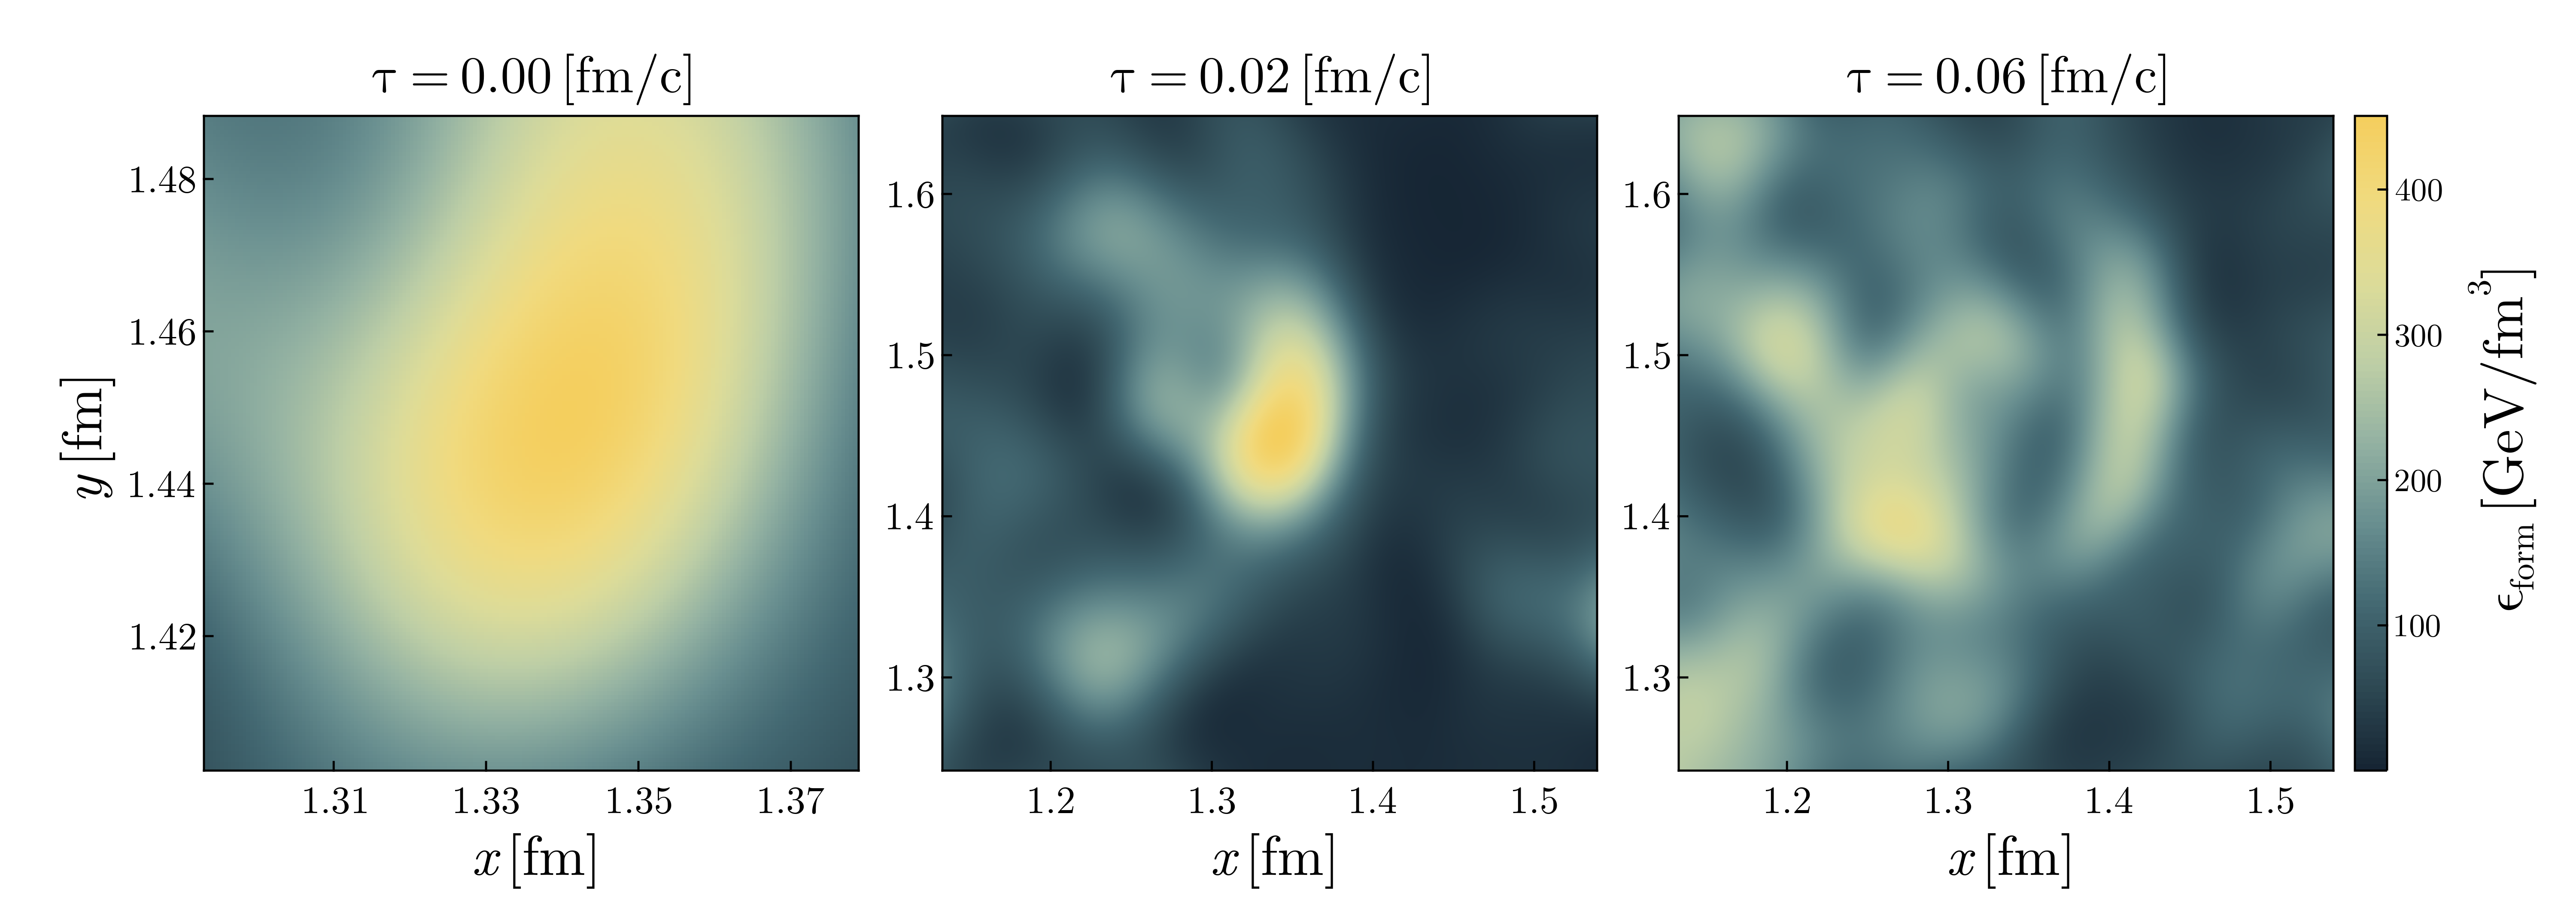
\includegraphics[width=0.8\textwidth]{images/hqs_flux_tubes_background.png}
%             }\only<2>{\includegraphics[width=0.8\textwidth]{images/hqs_flux_tubes_background+hqs.png}}
%         \end{figure}
%     \end{center}
% \end{frame}

% \section{The Glasma}
% \subsection{Color Glass Condensate}

% %%%%%%%%%%%%%%%%%%%%%%%%%%%%%%%%%%%%%%%%%%%
% %%%%%%%%%%%%%%%%% SLIDE X %%%%%%%%%%%%%%%%%
% %%%%%%%%%%%%%%%%%%%%%%%%%%%%%%%%%%%%%%%%%%%


% \setbeamertemplate{background}{
% \tikz[overlay,remember picture] \node[opacity=0.15, at=(current page.center)] {
%    \includegraphics[height=0.85\paperheight]{img/fig1_overview.pdf}};
% }
% \begin{frame}[plain,noframenumbering]{}
%     \begin{center}
%         \vspace{1cm}
%         {\large\color{normal}Part 1}\\[0.3cm]
%         {\huge\color{destacado}The Glasma}
%     \end{center}
% \end{frame}
% \setbeamertemplate{background}{}

% %%%%%%%%%%%%%%%%%%%%%%%%%%%%%%%%%%%%%%%%%%%
% %%%%%%%%%%%%%%%%% SLIDE 4 %%%%%%%%%%%%%%%%%
% %%%%%%%%%%%%%%%%%%%%%%%%%%%%%%%%%%%%%%%%%%%

% \begin{frame}
%     \frametitle{High energy QCD}
%     \framesubtitle{Glons as main degrees of freedom}
%         % \begin{center}
%         %     Initial stage using {\color{customblue}Color Glass Condensate} $\leftrightarrow$ EFT for high energy QCD \\
%         %     High energy nucleus $\leadsto$ many gluons 
%         %     % $\Leftrightarrow$ high occupation numbers for gluon fields \\ 
%         %     $\Rightarrow$ classical colored fields $\equiv$ {\color{custompink}Glasma}
%         % \end{center}
%     % \vspace{-0.2cm}
%     \begin{figure}[!hbt]
%         \centering
%     	\includegraphics[width=0.7\textwidth]{images/qcd_1.png}
%         \captionsetup{justification=centering}
%         \vspace{-0.2em}
%         \caption{\scriptsize\itshape Figure credits to T. Ullrich}
%     \end{figure}
% \end{frame}

% \begin{frame}[noframenumbering]
%     \frametitle{High energy QCD}
%     \framesubtitle{Glons as main degrees of freedom}
%         % \begin{center}
%         %     Initial stage using {\color{customblue}Color Glass Condensate} $\leftrightarrow$ EFT for high energy QCD \\
%         %     High energy nucleus $\leadsto$ many gluons 
%         %     % $\Leftrightarrow$ high occupation numbers for gluon fields \\ 
%         %     $\Rightarrow$ classical colored fields $\equiv$ {\color{custompink}Glasma}
%         % \end{center}
%     % \vspace{-0.2cm}
%     \begin{figure}[!hbt]
%         \centering
%     	\includegraphics[width=0.7\textwidth]{images/qcd_2.png}
%         \captionsetup{justification=centering}
%         \vspace{-0.2em}
%         \caption{\scriptsize\itshape Figure credits to T. Ullrich}
%     \end{figure}
% \end{frame}


% %%%%%%%%%%%%%%%%%%%%%%%%%%%%%%%%%%%%%%%%%%%%%
% %%%%%%%%%%%%%%%%%% SLIDE 5 %%%%%%%%%%%%%%%%%%
% %%%%%%%%%%%%%%%%%%%%%%%%%%%%%%%%%%%%%%%%%%%%%

% \subsection{Features of the Glasma fields}

% \begin{frame}
%     \frametitle{CGC as an EFT for high energy QCD}
%     \framesubtitle{Classical Yang-Mills fields}
%     \begin{columns}
%     \begin{column}{0.1\textwidth}\end{column}
%     \begin{column}{0.4\textwidth}
%         \begin{figure}[!hbt]
%             \centering
%             \includegraphics[width=\textwidth]{images/small_large_x.png}
%             \captionsetup{justification=centering}
%             \vspace{-0.2em}
%         \end{figure}
%     \end{column}
%     \begin{column}{0.5\textwidth}
%         \vspace{-1.3cm}
%         \begin{center}
%             Separation of scales between\\
%             {\color{customgreen}small-{\tiny $x$}} and {\color{custompink}large-{\huge $x$}} degrees of freedom
%         \end{center}
%     \end{column}
%     \begin{column}{0.1\textwidth}\end{column}
%     \end{columns}

%     % \begin{center}
%     %     Separation of scales between {\color{customgreen}small-{\tiny $x$}} and {\color{custompink}large-{\huge $x$}} degrees of freedom\\
%     %  {\color{customgreen}Small-{\tiny $x$}} $\Leftrightarrow$ classical gluon fields $\mapsto$ {\color{customblue}Yang-Mills} equations with sources $\Leftrightarrow$ {\color{custompink}large-{\huge $x$}}
%     % \end{center}
%      \vspace{-0.5cm}
%      \renewcommand{\eqnhighlightheight}{\vphantom{\mathcal{D}_\mu}\mathstrut}\begin{equation*}
%             \hspace{-3cm}\text{CYM equations: }\Big(\eqnmark[starrymain]{dmu}{\mathcal{D}_\mu}\eqnmark[starrysecond]{fmunu}{F^{\mu\nu}}\Big)\Big[\eqnmark[customgreen]{amu}{A^\mu}\Big]=\eqnmark[custompink]{jnu}{J^\nu}
%             \end{equation*}
%             \annotate[yshift=0.7em]{above, left}{dmu}{covariant derivative}
%             \annotate[yshift=0.7em]{above}{fmunu}{field strength tensor}
%             \annotate[yshift=-0.5em]{below, left}{amu}{gluons gauge field}
%             \annotate[yshift=-0.5em]{below, right}{jnu}{color current of nucleus}
%    \begin{center}
%     \vspace{-0.4cm}
%         \renewcommand{\eqnhighlightheight}{\vphantom{\delta^{\mu+}}\mathstrut}
%         \begin{equation*}
%             \eqnmark[customblue]{MV}{\text{MV model}}\text{and LC kinematics} \Rightarrow J^{\mu,a}(x)\propto
%             \delta^{\mu+}\eqnmark[custompink]{rho}{\rho^a}(x^-,\boldsymbol{x}_\perp)
%             \end{equation*}
%             \annotate[yshift=-0.1em]{below, left}{MV}{large nuclei}
%             \annotate[yshift=-0.1em]{below, right}{rho}{stochastic variable}
%         \\[0.1cm]
%         Two-point function $\langle {\color{custompink}\rho^a\rho^a}\rangle \propto {\color{customgreen} Q}^2_{\color{customgreen}s}$ {\color{customgreen}saturation momentum}   
%     \end{center}
% \end{frame}


% \begin{frame}[noframenumbering]
%     \frametitle{CGC as an EFT for high energy QCD}
%     \framesubtitle{Gauge fields before the collision}
%         % \begin{center}
%         %     Initial stage using {\color{customblue}Color Glass Condensate} $\leftrightarrow$ EFT for high energy QCD \\
%         %     High energy nucleus $\leadsto$ many gluons 
%         %     % $\Leftrightarrow$ high occupation numbers for gluon fields \\ 
%         %     $\Rightarrow$ classical colored fields $\equiv$ {\color{custompink}Glasma}
%         % \end{center}
%     % \vspace{-0.2cm}
%     \begin{figure}[!hbt]
%         \centering
%     	\includegraphics[width=0.7\textwidth]{images/cgc_nuclei.png}
%         \captionsetup{justification=centering}
%     \end{figure}
% \end{frame}



% %%%%%%%%%%%%%%%%%%%%%%%%%%%%%%%%%%%%%%%%%%%%%
% %%%%%%%%%%%%%%%%%% SLIDE 7 %%%%%%%%%%%%%%%%%%
% %%%%%%%%%%%%%%%%%%%%%%%%%%%%%%%%%%%%%%%%%%%%%

% % \addtocounter{framenumber}{-1}
% \begin{frame}
%     \frametitle{Collision of CGC nuclei}
%     \framesubtitle{Light-cone diagram of the collision}
%     \begin{columns}[onlytextwidth,t]
%        \column{.6\textwidth}
%        \begin{figure}
%             \centering
%             \includegraphics[width=0.7\columnwidth]{images/cgc_col.png}
%             % \vspace{-0.7cm}
%             \captionsetup{justification=centering}
%             % \caption{\scriptsize\itshape Figure credits to D. M\"{u}ller}
%         \end{figure}
%         \column{.35\textwidth}
%         \vspace{0.2cm}
%         \begin{center}
%             {\color{customgreen}$\sbullet[0.6]$ Known CGC fields} before the collision \\[0.1cm]
%             {\color{custompink}$\sbullet[0.6]$ Unknown Glasma fields} in the forward light-cone \\[0.5cm]
%             {\scriptsize{\color{lightgray}Milne coordinates ($\tau$, $\eta$)} \\
%             {\color{lightgray}$\tau=\sqrt{2 x^+x^-}$, $\eta=\ln(x^+/x^-)/2$}\\[0.4cm]
%             {\color{lightgray}Boost-invariant approximation $\mathrm{fields}=\mathrm{indep}(\eta)$} \\[0.3cm]
%             {\color{lightgray}Numerical solution of Yang-Mills}\\[-0.15cm] {\color{lightgray}equations $\Rightarrow$ Glasma}}
%         \end{center}
%         \column{.025\textwidth}
%     \end{columns}    
% \end{frame}


% %%%%%%%%%%%%%%%%%%%%%%%%%%%%%%%%%%%%%%%%%%%
% %%%%%%%%%%%%%%%%% SLIDE X %%%%%%%%%%%%%%%%%
% %%%%%%%%%%%%%%%%%%%%%%%%%%%%%%%%%%%%%%%%%%%


% \setbeamertemplate{background}{
% \tikz[overlay,remember picture] \node[opacity=0.15, at=(current page.center)] {
%    \includegraphics[width=\textwidth]{img/flux_tubes_auau_200_nums_1_dpi_300_nounits.png}};
% }
% \begin{frame}[plain,noframenumbering]{}
%     \begin{center}
%         \vspace{1cm}
%         {\large\color{normal}Part 2}\\[0.3cm]
%         {\huge\color{destacado}Features of the Glasma}
%     \end{center}
% \end{frame}
% \setbeamertemplate{background}{}


% %%%%%%%%%%%%%%%%%%%%%%%%%%%%%%%%%%%%%%%%%%%%%
% %%%%%%%%%%%%%%%%%% SLIDE 8 %%%%%%%%%%%%%%%%%%
% %%%%%%%%%%%%%%%%%%%%%%%%%%%%%%%%%%%%%%%%%%%%%

% % \addtocounter{framenumber}{-1}
% \begin{frame}
%     \frametitle{The Glasma fields}
%     \framesubtitle{General features}
%     \begin{figure}
%         \centering
%         \includegraphics[width=0.9\textwidth]{img/flux_tubes_auau_200_nums_1_dpi_300_nounits.png}
%         \captionsetup{justification=centering}
%         \caption{Relevant scale ${\color{custompink}Q_s}$ \\
%         {\scriptsize\itshape Fields {\color{customgreen}dilute} after $\delta\tau\simeq {\color{custompink}Q}^{-1}_{\color{custompink}s}$, arrange themselves in {\color{customgreen}correlation domains} of $\delta x_T \simeq {\color{custompink}Q}^{-1}_{\color{custompink}s}$} 
%         % \\[0.2cm]
%         % {\color{customblue}Boost-invariant} and {\color{customblue}anisotropic} field configurations
%         }
%     \end{figure}
% \end{frame}

% \begin{frame}[noframenumbering]
%     \frametitle{The Glasma fields}
%     \framesubtitle{Bjorken expansion}
%     {\transparent{0.1}\begin{figure}
%         \centering
%         \includegraphics[width=0.9\textwidth]{img/flux_tubes_auau_200_nums_1_dpi_300_nounits.png}
%         \captionsetup{justification=centering}
%         \caption{Relevant scale ${\color{custompink}Q_s}$ \\
%         {\scriptsize\itshape Fields {\color{customgreen}dilute} after $\delta\tau\simeq {\color{custompink}Q}^{-1}_{\color{custompink}s}$, arrange themselves in {\color{customgreen}correlation domains} of $\delta x_T \simeq {\color{custompink}Q}^{-1}_{\color{custompink}s}$} 
%         % \\[0.2cm]
%         % {\color{customblue}Boost-invariant} and {\color{customblue}anisotropic} field configurations
%         }
%     \end{figure}}
%     \begin{center}
%         \begin{tikzpicture}[remember picture,overlay]
%             \node[align=center] at (0,4) {
%                 The fields become {\color{customgreen}dilute} after $\delta\tau\simeq {\color{custompink}Q}^{-1}_{\color{custompink}s}$\\
%                 \includegraphics[width=0.55\textwidth]{images/dilute_2.png}
%             };
%         \end{tikzpicture} 
%     \end{center}
% \end{frame}


% \begin{frame}[noframenumbering]
%     \frametitle{The Glasma fields}
%     \framesubtitle{Flux tubes}
%     {\transparent{0.1}\begin{figure}
%         \centering
%         \includegraphics[width=0.9\textwidth]{img/flux_tubes_auau_200_nums_1_dpi_300_nounits.png}
%         \captionsetup{justification=centering}
%         \caption{Relevant scale ${\color{custompink}Q_s}$ \\
%         {\scriptsize\itshape Fields {\color{customgreen}dilute} after $\delta\tau\simeq {\color{custompink}Q}^{-1}_{\color{custompink}s}$, arrange themselves in {\color{customgreen}correlation domains} of $\delta x_T \simeq {\color{custompink}Q}^{-1}_{\color{custompink}s}$} 
%         % \\[0.2cm]
%         % {\color{customblue}Boost-invariant} and {\color{customblue}anisotropic} field configurations
%         }
%     \end{figure}}
%     \vspace{0.3cm}
%     \begin{center}
%         \begin{tikzpicture}[remember picture,overlay]
%             \node[align=center] at (0,4) {
%                 The fields arrange themselves in {\color{customgreen}correlation domains} of $\delta x_T \simeq {\color{custompink}Q}^{-1}_{\color{custompink}s}$\\
%                 \includegraphics[width=0.48\textwidth]{images/correlation_2.png}
%             };
%         \end{tikzpicture} 
%     \end{center}
% \end{frame}


% \begin{frame}[noframenumbering]
%     \frametitle{The Glasma fields}
%     \framesubtitle{Anisotropy}
%     {\transparent{0.1}\begin{figure}
%         \centering
%         \includegraphics[width=0.9\textwidth]{img/flux_tubes_auau_200_nums_1_dpi_300_nounits.png}
%         \captionsetup{justification=centering}
%         \caption{Relevant scale ${\color{custompink}Q_s}$ \\
%         {\scriptsize\itshape Fields {\color{customgreen}dilute} after $\delta\tau\simeq {\color{custompink}Q}^{-1}_{\color{custompink}s}$, arrange themselves in {\color{customgreen}correlation domains} of $\delta x_T \simeq {\color{custompink}Q}^{-1}_{\color{custompink}s}$} 
%         % \\[0.2cm]
%         % {\color{customblue}Boost-invariant} and {\color{customblue}anisotropic} field configurations
%         }
%     \end{figure}}
%     \vspace{0.3cm}
%     \begin{center}
%         \begin{tikzpicture}[remember picture,overlay]
%             \node[align=center] at (0,4) {
%                 Longitudinal $\neq$ transverse $\Rightarrow$ {\color{pinky}anisotropy}\\
%                 \includegraphics[width=0.55\textwidth]{images/anisotropy.png}
%             };
%         \end{tikzpicture} 
%     \end{center}
% \end{frame}

% \section{Hard probes in the Glasma}

% \setbeamertemplate{background}{
% \tikz[overlay,remember picture] \node[opacity=0.15, at=(current page.center)] {
%    \includegraphics[height=0.8\paperheight]{img/momentum_broadening_flipped.pdf}};
% }
% \begin{frame}[plain,noframenumbering]{}
%     \begin{center}
%         \vspace{1cm}
%         {\large\color{normal}Part 3}\\[0.3cm]
%         {\huge\color{destacado}Hard probes in the Glasma}
%     \end{center}
% \end{frame}
% \setbeamertemplate{background}{}

% \subsection{Classical transport}

% %%%%%%%%%%%%%%%%%%%%%%%%%%%%%%%%%%%%%%%%%%%%%
% %%%%%%%%%%%%%%%%%% SLIDE 9 %%%%%%%%%%%%%%%%%%
% %%%%%%%%%%%%%%%%%%%%%%%%%%%%%%%%%%%%%%%%%%%%%

% \begin{frame}
%     \frametitle{Particles in Yang-Mills fields}
%     \framesubtitle{Wong's equations of motion}
%    \begin{center}
%        Wong's equations $\leftrightarrow$ classical equations of motion for particles $({\color{customblue}x^\mu},{\color{customred}p^\mu},{\color{customyellow}Q})$ \\
%     evolving in a Yang-Mills background field ${\color{starrysecond}A^\mu}$
%    \end{center} 
%         \vspace{1cm}
%         \renewcommand{\eqnhighlightheight}{\vphantom{x}}
%         \begin{equation*}
%             \frac{\d}{\d\hspace{-0.1cm}\eqnmark[destacado]{tau}{\boldsymbol{\tau}}\hspace{-0.2cm}}\eqnmark[customblue]{xmu}{x^\mu}=\frac{{\color{customred}p^\mu}}{\eqnmark[destacado]{m}{m}},\qquad \eqnmark[destacado]{Ddtau}{\frac{\mathrm{D}}{\d\boldsymbol{\tau}}}\hspace{-0.2cm}\eqnmark[customred]{pmu}{p^\mu}=2\hspace{-0.1cm}\eqnmark[destacado]{g}{g}\hspace{-0.1cm}\tr{{\color{customyellow}Q}F^{\mu\nu}[\hspace{-0.1cm}\eqnmark[starrysecond]{amu}{A^\mu}\hspace{-0.1cm}]}\frac{{\color{customred}p_\nu}}{m},\qquad 
%             \underbrace{\frac{\d}{\d\boldsymbol{\tau}}\hspace{-0.1cm}\eqnmark[customyellow]{Q}{Q}\hspace{-0.1cm}=-\mathrm{i}g [{\color{starrysecond}A_\mu},{\color{customyellow}Q}]\,\frac{{\color{customred}p^\mu}}{m}}_{\substack{\text{\footnotesize color rotation}\,\rightarrow\,{\color{customgreen}\mathcal{U}}\in\,\mathrm{SU(3)} \\[0.2cm] {\color{customyellow}Q}(\boldsymbol{\tau})=\,{\color{customgreen}\mathcal{U}}(\boldsymbol{\tau},\boldsymbol{\tau}^\prime){\color{customyellow}Q}(\boldsymbol{\tau^\prime})\,{\color{customgreen}\mathcal{U}^\dagger}(\boldsymbol{\tau},\boldsymbol{\tau}^\prime)}}
%             \end{equation*}
%             \annotate[yshift=1.2em]{above}{xmu}{coordinate}
%             \annotate[yshift=1.2em]{above}{pmu}{momentum}
%             \annotate[yshift=-0.5em]{below, right}{m}{\tiny mass}
%             \annotate[yshift=-1.5em]{below, right}{Ddtau}{\tiny covariant derivative}
%             \annotate[yshift=-1.5em]{below, right}{tau}{\tiny proper time}
%             \annotate[yshift=-0.7em]{below, right}{g}{\tiny coupling constant}
%             \annotate[yshift=1.2em]{above}{Q}{color charge}
%             \annotate[yshift=1.2em]{above, right}{amu}{gauge field}
%        \\
%         \begin{center}
%             Symplectic numerical solver $\xrightarrow{\mathrm{assures}}$ ${\color{customyellow}Q}\in\mathrm{SU(3)}$, conservation of Casimir invariants 
%         \end{center} 
% \end{frame}

% \begin{frame}[noframenumbering]
%     \frametitle{Particles in Yang-Mills fields}
%     \framesubtitle{Wong's equations of motion}
%     {\transparent{0.1}\begin{center}
%        Wong's equations $\leftrightarrow$ classical equations of motion for particles $({\color{customblue}x^\mu},{\color{customred}p^\mu},{\color{customyellow}Q})$ \\
%     evolving in a Yang-Mills background field ${\color{starrysecond}A^\mu}$
%    \end{center} 
%         \vspace{1cm}
%         \renewcommand{\eqnhighlightheight}{\vphantom{x}}
%         \begin{equation*}
%             \frac{\d}{\d\hspace{-0.1cm}\eqnmark[destacado]{tau}{\boldsymbol{\tau}}\hspace{-0.2cm}}\eqnmark[customblue]{xmu}{x^\mu}=\frac{{\color{customred}p^\mu}}{\eqnmark[destacado]{m}{m}},\qquad \eqnmark[destacado]{Ddtau}{\frac{\mathrm{D}}{\d\boldsymbol{\tau}}}\hspace{-0.2cm}\eqnmark[customred]{pmu}{p^\mu}=2\hspace{-0.1cm}\eqnmark[destacado]{g}{g}\hspace{-0.1cm}\tr{{\color{customyellow}Q}F^{\mu\nu}[\hspace{-0.1cm}\eqnmark[starrysecond]{amu}{A^\mu}\hspace{-0.1cm}]}\frac{{\color{customred}p_\nu}}{m},\qquad 
%             \underbrace{\frac{\d}{\d\boldsymbol{\tau}}\hspace{-0.1cm}\eqnmark[customyellow]{Q}{Q}\hspace{-0.1cm}=-\mathrm{i}g [{\color{starrysecond}A_\mu},{\color{customyellow}Q}]\,\frac{{\color{customred}p^\mu}}{m}}_{\substack{\text{\footnotesize color rotation}\,\rightarrow\,{\color{customgreen}\mathcal{U}}\in\,\mathrm{SU(3)} \\[0.2cm] {\color{customyellow}Q}(\boldsymbol{\tau})=\,{\color{customgreen}\mathcal{U}}(\boldsymbol{\tau},\boldsymbol{\tau}^\prime){\color{customyellow}Q}(\boldsymbol{\tau^\prime})\,{\color{customgreen}\mathcal{U}^\dagger}(\boldsymbol{\tau},\boldsymbol{\tau}^\prime)}}
%             \end{equation*}
%             \annotate[yshift=1.2em]{above}{xmu}{coordinate}
%             \annotate[yshift=1.2em]{above}{pmu}{momentum}
%             \annotate[yshift=-0.5em]{below, right}{m}{\tiny mass}
%             \annotate[yshift=-1.5em]{below, right}{Ddtau}{\tiny covariant derivative}
%             \annotate[yshift=-1.5em]{below, right}{tau}{\tiny proper time}
%             \annotate[yshift=-0.7em]{below, right}{g}{\tiny coupling constant}
%             \annotate[yshift=1.2em]{above}{Q}{color charge}
%             \annotate[yshift=1.2em]{above, right}{amu}{gauge field}
%        \\
%         \begin{center}
%             Symplectic numerical solver $\xrightarrow{\mathrm{assures}}$ ${\color{customyellow}Q}\in\mathrm{SU(3)}$, conservation of Casimir invariants 
%         \end{center}}
%         \begin{center}
%             \vspace{40pt}
%             \begin{tikzpicture}[remember picture,overlay]
%                 \node[align=center] at (0,4) {
%                     \large Boltzmann-Vlasov collisionless non-Abelian plasma\\[10pt]
%                     \large ${\color{customred}p^\mu}[\partial_\mu+g {\color{customyellow}Q^a} {\color{starrysecond}F^{\mu\nu}}({\color{customblue}x^\mu})\partial^\nu_{{\color{customred}p^\mu}}+gf^{abc}{\color{starrysecond}A^b_\mu}({\color{customblue}x^\mu}){\color{customyellow}Q^c}\partial_{{\color{customyellow}Q^a}}]\boldsymbol{f}({\color{customblue}x^\mu}, {\color{customred}p^\mu}, {\color{customyellow}Q^a})=0$\\[30pt]
%                     \large $\boldsymbol{f}({\color{customblue}x^\mu}, {\color{customred}p^\mu}, {\color{customyellow}Q^a})\xrightarrow{\text{sample}}$ test particles $({\color{customblue}x^\mu}, {\color{customred}p^\mu}, {\color{customyellow}Q^a})$\\[10pt]
%                     \large $\Rightarrow$ Wong's equations
%                 };
%             \end{tikzpicture} 
%         \end{center}
% \end{frame}


% %%%%%%%%%%%%%%%%%%%%%%%%%%%%%%%%%%%%%%%%%%%%%
% %%%%%%%%%%%%%%%%%% SLIDE 10 %%%%%%%%%%%%%%%%%%
% %%%%%%%%%%%%%%%%%%%%%%%%%%%%%%%%%%%%%%%%%%%%%

% \begin{frame}[noframenumbering]
%     \frametitle{Particles in Yang-Mills fields}
%     \framesubtitle{Vizualizing the trajectories}
%     \vspace{-0.5cm}
%     \begin{columns}[onlytextwidth,t]
%         \column{.025\textwidth}
%        \column{.3\textwidth}
%                 \begin{center}
%                     Change of coordinates 
%                 \end{center}
%                 \vspace{-20pt}
%                 \begin{figure}[!hbt]
%                     \centering
%                 \includegraphics[width=1.1\columnwidth]{images/wong_coord.png}
%                 \end{figure}
%                 \column{.025\textwidth}
%         \column{.3\textwidth}
%             \begin{center}
%                 Color Lorentz force
%             \end{center}
%             \vspace{-20pt}
%             \begin{figure}[!hbt]
%                 \centering
%                 \includegraphics[width=1.1\columnwidth]{images/wong_mom.png}
%             \end{figure}
%             \column{.025\textwidth}
%         \column{.3\textwidth}
%             \begin{center}
%                 Color rotation
%             \end{center}
%             \vspace{-15pt}
%             \begin{figure}[!hbt]
%                 \centering
%                 \includegraphics[width=1.05\columnwidth]{images/wong_charge.png}
%             \end{figure}
%             \column{.025\textwidth}
%     \end{columns}
% \end{frame}

% \subsection{Momentum broadening}

% %%%%%%%%%%%%%%%%%%%%%%%%%%%%%%%%%%%%%%%%%%%%%
% %%%%%%%%%%%%%%%%%% SLIDE 7 %%%%%%%%%%%%%%%%%%
% %%%%%%%%%%%%%%%%%%%%%%%%%%%%%%%%%%%%%%%%%%%%%

% \begin{frame}
%     \frametitle{Quantifying the effect of Glasma}
%     \framesubtitle{Momentum broadening}
%     \begin{columns}[onlytextwidth,t]
%         \column{.03\textwidth}
%        \column{.45\textwidth}
%         \vspace{-15pt}
%        \begin{figure}
%             \centering
%             \includegraphics[width=\columnwidth]{img/hqs_trajectories.png}
%             % \vspace{-0.7cm}
%             \captionsetup{justification=centering}
%             % \caption{\scriptsize\itshape Figure credits to D. M\"{u}ller}
%         \end{figure}
%         \column{.08\textwidth}
%         \column{.4\textwidth}
%         \vspace{0.2cm}
%         \begin{center}
%             {\color{ming}Momentum broadening} 
%             \begin{equation*}
%                 {\color{ming}\delta p_i^2}(\tau)\equiv p_i^2(\tau)-p_i^2(\tau_\mathrm{form})
%             \end{equation*}
%             Instantaneous {\color{customyellow}transport coefficient}
%             \begin{equation*}
%                 \frac{\d }{\d\tau}\langle\delta p^2_i(\tau)\rangle\equiv \begin{cases}{\color{customyellow}\kappa_i}(\tau),&\text{heavy quarks}\\
%                 {\color{customyellow}\hat{q}_i}(\tau),&\text{jets}\end{cases}
%             \end{equation*}
%             {\color{customblue}Anisotropy} $\equiv$ ${\color{customblue}\langle\delta p_L^2\rangle/\langle\delta p_T^2\rangle}$
            
%         \end{center}
%         \column{.05\textwidth}
%     \end{columns}    
% \end{frame}


% %%%%%%%%%%%%%%%%%%%%%%%%%%%%%%%%%%%%%%%%%%%%%
% %%%%%%%%%%%%%%%%%% SLIDE 12 %%%%%%%%%%%%%%%%%%
% %%%%%%%%%%%%%%%%%%%%%%%%%%%%%%%%%%%%%%%%%%%%%

% \begin{frame}
%     \frametitle{Heavy quarks in Glasma}
%     \framesubtitle{Momentum broadening and $\kappa$}
%     \vspace{5pt}
%     \begin{center}
%         \begin{figure}[!hbt]
%         \centering
%         \includegraphics[width=1.6\textheight]{images/hp23_mom_broad_kappa_anis_wong_vs_kappa.pdf}
%         \end{figure}
%         \end{center}
%     \end{frame}


% %%%%%%%%%%%%%%%%%%%%%%%%%%%%%%%%%%%%%%%%%%%%%
% %%%%%%%%%%%%%%%%%% SLIDE 12 %%%%%%%%%%%%%%%%%%
% %%%%%%%%%%%%%%%%%%%%%%%%%%%%%%%%%%%%%%%%%%%%%

% \begin{frame}
%     \frametitle{Jets in Glasma}
%     \framesubtitle{Momentum broadening and $\hat{q}$}
%     \vspace{5pt}
%     \begin{center}
%         \begin{figure}[!hbt]
%         \centering
%         \includegraphics[width=1.6\textheight]{images/hp23_mom_broad_qhat_anis_wong_vs_qhat.pdf}
%         \end{figure}
%         \end{center}
%     \end{frame}


% %%%%%%%%%%%%%%%%%%%%%%%%%%%%%%%%%%%%%%%%%%%%%
% %%%%%%%%%%%%%%%%%% SLIDE 15 %%%%%%%%%%%%%%%%%%
% %%%%%%%%%%%%%%%%%%%%%%%%%%%%%%%%%%%%%%%%%%%%%


% \begin{frame}
%     \frametitle{Large transport coefficients}
%     \framesubtitle{Plausible in an EKT framework}
%     \vspace{-0.4cm}
%     \begin{columns}[onlytextwidth,t]
%     \column{.5\textwidth}
%         \begin{figure}[!hbt]
%             \centering
%             \captionsetup{justification=centering}
%             \caption{Schematic evolution of $\hat{q}$}\vspace{-0.3cm}
%             \includegraphics[width=0.8\columnwidth]{img/qhat_schematic_evolution.pdf}\vspace{-0.3cm}
%             \caption{\scriptsize\itshape Figure from \href{https://arxiv.org/abs/2303.12595}{\color{ForestGreen}[2303.12595]}}
%         \end{figure}
%     \column{.5\textwidth}
%         \begin{figure}[!hbt]
%             \centering
%             \captionsetup{justification=centering}
%             \caption{{\color{ForestGreen}Kinetic theory}$^*$ connects the large $\hat{q}$ in {\color{Dandelion}Glasma}\\ to subsequent {\color{Periwinkle}hydrodynamics}}\vspace{-0.2cm}
%             \includegraphics[width=0.8\columnwidth]{img/2023-03-07-16-41-35_qhat_appetizer_glasma_comparison_493.pdf}
%         \end{figure}
%     \end{columns}   
% \end{frame}

% \begin{frame}[noframenumbering]
%     \frametitle{Large transport coefficients}
%     \framesubtitle{Plausible in an EKT framework}
%     \vspace{-0.4cm}
%     \begin{columns}[onlytextwidth,t]
%     \column{.5\textwidth}
%         \begin{figure}[!hbt]
%             \centering
%             \captionsetup{justification=centering}
%             \caption{Schematic evolution of $\hat{q}$}\vspace{-0.3cm}
%             \includegraphics[width=0.78\columnwidth]{img/qhat_schematic_evolution.pdf}\vspace{-0.3cm}
%             \caption{\scriptsize\itshape Figure from \href{https://arxiv.org/abs/2303.12595}{\color{ForestGreen}[2303.12595]}}
%         \end{figure}
%     \column{.5\textwidth}
%         \begin{figure}[!hbt]
%             \centering
%             \captionsetup{justification=centering}
%             \caption{{\color{ForestGreen}Kinetic theory}$^*$ connects the large $\hat{q}$ in {\color{Dandelion}Glasma}\\ to subsequent {\color{Periwinkle}hydrodynamics}}\vspace{-0.2cm}
%             \includegraphics[width=0.8\columnwidth]{images/qhat_whole.png}
%         \end{figure}
%     \end{columns}   
% \end{frame}


% \section{Observables}

% \setbeamertemplate{background}{
% \tikz[overlay,remember picture] \node[opacity=0.15, at=(current page.center)] {
%    \includegraphics[height=0.8\paperheight]{images/Cdetadphi_3D_toy_charm_pT_1_tau_0.1_crop.png}};
% }
% \begin{frame}[plain,noframenumbering]{}
%     \begin{center}
%         \vspace{1cm}
%         {\large\color{normal}Part 4}\\[0.3cm]
%         {\huge\color{destacado}Phenomenology}
%     \end{center}
% \end{frame}
% \setbeamertemplate{background}{}

% \subsection{Two particle correlations}

% \begin{frame}
%     \frametitle{Two particle correlations}
%     \framesubtitle{Sketch of $Q\overline{Q}$ pairs in the Glasma}
%     \begin{center}
%     \vspace{0.6cm}
%     % : initial particle $p_T$ and Glasma $Q_s$\\[0.5cm]
%     $\text{Control parameters: }\eqnmark[jyublue]{glasma}{\text{saturation momentum $Q_s$}} \text{ and }\eqnmark[pinky]{probes}{\text{initial $p_T$}}\text{\footnotesize with $\tau_\mathrm{form}=1/(2 m_T)$}$
%     \annotate[yshift=1em]{above,left}{glasma}{\text{Glasma fields}}
%     \annotate[yshift=1em]{above}{probes}{\text{heavy quarks}}
%     \\[0.2cm]
%     \begin{figure}[!hbt]
%         \centering
%         \includegraphics[width=0.95\textwidth]{images/sketch_quark_pair_evo_v2.png}
%     \end{figure}
%     \end{center}
% \end{frame}


% \begin{frame}[noframenumbering]
%     \frametitle{Two particle correlations}
%     \framesubtitle{Quantifying the decorrelation}
%     \vspace{5pt}
%     \begin{center}
%     {\color{pinky}Rapidity} and {\color{pinky}azimuthal} correlations ${\color{pinky}\mathcal{C}(\Delta\eta, \Delta\phi)}\equiv\dfrac{1}{N_\mathrm{pairs}}\dfrac{\mathrm{d}^2 N}{\mathrm{d}\Delta\eta \mathrm{d}\Delta\phi}$ \\[0.3cm]
%     {\color{customblue}Initial} $\mathcal{C}(\tau_\mathrm{form})\propto{\color{customblue}\delta(\Delta\phi-\pi)\delta(\Delta\eta)}\xmapsto{\Delta\tau\text{ in Glasma}}\mathcal{C}(\tau_\mathrm{form}+\Delta\tau)\xRightarrow{\text{extract}}{\color{pinky}\sigma_{\Delta\phi}}(\Delta\tau), {\color{pinky}\sigma_{\Delta\eta}}(\Delta\tau)$ 

%     % \vspace{-10pt}
%     \begin{figure}[!hbt]
%     \centering
%     \includegraphics[width=\textwidth]{images/sketch_decorrelation_v2_crop.png}
%     \end{figure}
%     \end{center}
% \end{frame}

% \begin{frame}
%     \frametitle{Azimuthal decorrelation width}
%     \framesubtitle{Effect of heavy quark $p_T$ and Glasma $Q_s$}
%     \begin{center}
%         \begin{columns}[onlytextwidth,t]
%             \column{.02\textwidth}
%            \column{.47\textwidth}
%            \begin{figure}
%                 \centering
%                 \vspace{5pt}
%                 \includegraphics[width=\columnwidth]{images/sigma_dphideta_tau_charm_beauty_pT_dep_final_azimuth.png}
%                 % \captionsetup{justification=centering}
%                 % \caption{\scriptsize\itshape EPPS16 nuclear PDF from \href{https://arxiv.org/abs/1612.05741}{\color{ForestGreen}[1612.05741]}}
%                 % \vspace{-0.7cm}
%             \end{figure}
%             \column{.02\textwidth}
%             \column{.47\textwidth}
%             \vspace{-17pt}
%             \begin{figure}
%                 \centering
%                 \includegraphics[width=1.02\columnwidth]{images/sigma_dphideta_tau_charm_beauty_Qs_dep_scaled_final_azimuth.png}
%                 % \vspace{-0.7cm}
%                 % \captionsetup{justification=centering}
%                 % \caption{\scriptsize\itshape Figure credits to D. M\"{u}ller}
%             \end{figure}
%             \column{.02\textwidth}
%         \end{columns}    
%     \end{center}

%     % \begin{center}
%     %     \begin{figure}[!hbt]
%     %         \centering
%     %         \includegraphics[width=0.9\textwidth]{images/sigma_dphideta_tau_charm_beauty_pT_dep_final.png}
%     %     \end{figure}
%     % \end{center}
% \end{frame}

% \begin{frame}[noframenumbering]
%     \frametitle{Azimuthal decorrelation width}
%     \framesubtitle{Effect of heavy quark $p_T$ and Glasma $Q_s$}
%     {\transparent{0.1}\begin{center}
%         \begin{columns}[onlytextwidth,t]
%             \column{.02\textwidth}
%            \column{.47\textwidth}
%            \begin{figure}
%                 \centering
%                 \vspace{5pt}
%                 \includegraphics[width=\columnwidth]{images/sigma_dphideta_tau_charm_beauty_pT_dep_final_azimuth.png}
%                 % \captionsetup{justification=centering}
%                 % \caption{\scriptsize\itshape EPPS16 nuclear PDF from \href{https://arxiv.org/abs/1612.05741}{\color{ForestGreen}[1612.05741]}}
%                 % \vspace{-0.7cm}
%             \end{figure}
%             \column{.02\textwidth}
%             \column{.47\textwidth}
%             \vspace{-17pt}
%             \begin{figure}
%                 \centering
%                 \includegraphics[width=1.02\columnwidth]{images/sigma_dphideta_tau_charm_beauty_Qs_dep_scaled_final_azimuth.png}
%                 % \vspace{-0.7cm}
%                 % \captionsetup{justification=centering}
%                 % \caption{\scriptsize\itshape Figure credits to D. M\"{u}ller}
%             \end{figure}
%             \column{.02\textwidth}
%         \end{columns}    
%     \end{center}}
%     \begin{center}
%         % \vspace{10pt}
%         \begin{tikzpicture}[remember picture,overlay]
%             \node[align=center] at (0,4.5) {
%             \Large {\color{customblue}Significant decorrelaton} for $Q\overline{Q}$ pairs with\\[0.2cm]
%             \Large sufficiently {\color{pinky}small initial $p_T$} and {\color{jyublue}large $Q_s$}
%             };
%         \end{tikzpicture} 
%     \end{center}
% \end{frame}


% \begin{frame}
%     \frametitle{Phenomenology implications}
%     \framesubtitle{Azimuthal angle correlations}
%     \begin{center}
%         % \\[0.5cm]
%         \vspace{5pt}
%         {\color{pinky}First measurement} of azimuthal correlations in PbPb from \href{https://arxiv.org/abs/2308.16652}{\color{customblue}[ATLAS 2308.16652]} \\
%         \vspace{-10pt}
%         \begin{columns}[onlytextwidth,t]
%             \column{.02\textwidth}
%            \column{.47\textwidth}
%            \begin{figure}
%                 \centering
%                 \vspace{-5pt}
%                 \includegraphics[width=\columnwidth]{images/atlas_fig1_crop.png}
%                 % \captionsetup{justification=centering}
%                 % \caption{\scriptsize\itshape EPPS16 nuclear PDF from \href{https://arxiv.org/abs/1612.05741}{\color{ForestGreen}[1612.05741]}}
%                 % \vspace{-0.7cm}
%             \end{figure}
%             \column{.02\textwidth}
%             \column{.47\textwidth}
%             % \vspace{0.1cm}
%             \begin{figure}
%                 \centering
%                 \includegraphics[width=0.9\columnwidth]{images/atlas_fig2_crop.png}
%                 % \vspace{-0.7cm}
%                 % \captionsetup{justification=centering}
%                 % \caption{\scriptsize\itshape Figure credits to D. M\"{u}ller}
%             \end{figure}
%             \column{.02\textwidth}
%         \end{columns}    
%     \end{center}
% \end{frame}

% \begin{frame}[noframenumbering]
%     \frametitle{Phenomenology implications}
%     \framesubtitle{Azimuthal angle correlations}
%     {\transparent{0.1} \begin{center}
%         % \\[0.5cm]
%         \vspace{5pt}
%         {\color{pinky}First measurement} of azimuthal correlations in PbPb from \href{https://arxiv.org/abs/2308.16652}{\color{customblue}[ATLAS 2308.16652]} \\
%         \vspace{-10pt}
%         \begin{columns}[onlytextwidth,t]
%             \column{.02\textwidth}
%            \column{.47\textwidth}
%            \begin{figure}
%                 \centering
%                 \vspace{-5pt}
%                 \includegraphics[width=\columnwidth]{images/atlas_fig1_crop.png}
%                 % \captionsetup{justification=centering}
%                 % \caption{\scriptsize\itshape EPPS16 nuclear PDF from \href{https://arxiv.org/abs/1612.05741}{\color{ForestGreen}[1612.05741]}}
%                 % \vspace{-0.7cm}
%             \end{figure}
%             \column{.02\textwidth}
%             \column{.47\textwidth}
%             % \vspace{0.1cm}
%             \begin{figure}
%                 \centering
%                 \includegraphics[width=0.9\columnwidth]{images/atlas_fig2_crop.png}
%                 % \vspace{-0.7cm}
%                 % \captionsetup{justification=centering}
%                 % \caption{\scriptsize\itshape Figure credits to D. M\"{u}ller}
%             \end{figure}
%             \column{.02\textwidth}
%         \end{columns}    
%     \end{center}}
%     \begin{center}
%         \vspace{10pt}
%         \begin{tikzpicture}[remember picture,overlay]
%             \node[align=center] at (0,3.8) {
%             \Large No theoretical model predictions consider the {\color{customblue}inital stage}\\[1.0cm]
%             \Large The azimiuthal decorrelation $\sigma_{\Delta\phi}$ from {\color{pinky}Glasma} \\[0.2cm] \Large needs to be accounted for
%             };
%         \end{tikzpicture} 
%     \end{center}
% \end{frame}

% \subsection{Nuclear modification factor}


% %%%%%%%%%%%%%%%%%%%%%%%%%%%%%%%%%%%%%%%%%%%%%
% %%%%%%%%%%%%%%%%%% SLIDE 16 %%%%%%%%%%%%%%%%%%
% %%%%%%%%%%%%%%%%%%%%%%%%%%%%%%%%%%%%%%%%%%%%%

% \section{Highlights}
% \begin{frame}
%     \frametitle{Highlights}
%     \begin{center}
%         {\Large\color{customblue} Framework:}\\
%         Numerical solver for hard probes in Glasma
%         \\
%         \textbf{Anisotropic} momentum broadening\\
%         \textbf{Large} transport coefficients $\boldsymbol{\kappa}$ and $\boldsymbol{\hat{q}}$\\[0.5cm]

%         {\Large\color{customblue} Phenomenology:}\\
%         \textbf{Azimuthal decorrelation} of $Q\overline{Q}$ pairs\\
%         Nuclear modification factor $R_{AA}$ with \textbf{nPDFs}\\[0.5cm]
        
%         {\Large\color{customblue} Improvements:}\\
%         Energy loss
%     \end{center}
% \end{frame}

% \appendix

% \begin{frame}[plain,noframenumbering]{}
%     \vspace{20pt}
%     \huge\centering Thank you!
% \end{frame}

% \begin{frame}[plain,noframenumbering]{}
%     \huge\centering Back-up
% \end{frame}

% \subsection{Nuclear modification factor}

% \begin{frame}
%     \frametitle{Nuclear modification factor}
%     \framesubtitle{Sketch of $p_T$ spectra in the Glasma}
%     \begin{center}
%     \vspace{0.6cm}
%     % : initial particle $p_T$ and Glasma $Q_s$\\[0.5cm]
%     Heavy quarks $\xmapsto{\text{FONLL}^*}$ initial $p_T$ distribution $\propto\mathrm{d}\sigma^{pp/AA}/\mathrm{d}p_T(\sqrt{s}, \mathrm{PDF/nPDF})$
%     \\[0.2cm]
%     \begin{figure}[!hbt]
%         \centering
%         \includegraphics[width=0.95\textwidth]{images/sketch_dndpt_v3.png}
%     \end{figure}
%     \end{center}
%     \begin{center}
%         \scriptsize $^*$\textit{Fixed Order + Next-to-Leading Logarithms}, state-of-the-art resummed heavy quark production
%     \end{center}
% \end{frame}

% \begin{frame}[noframenumbering]
%     \frametitle{Nuclear modification factor}
%     \framesubtitle{Extraction of $R_{AA}$ in Glasma}
%     \begin{columns}[onlytextwidth,t]
%         % \column{.02\textwidth}
%        \column{.56\textwidth}
%         \vspace{-20pt}
%        \begin{figure}
%             \centering
%             \includegraphics[width=1.05\columnwidth]{images/sketch_raa_gl_fonll_v4.png}
%             % \vspace{-0.7cm}
%             \captionsetup{justification=centering}
%             % \caption{\scriptsize\itshape Figure credits to D. M\"{u}ller}
%         \end{figure}
%         \column{.02\textwidth}
%         \column{.4\textwidth}
%         \vspace{0.1cm}
%         \begin{center}
%             Glasma $p_T$ broadening $\Rightarrow {\color{customblue}\dfrac{\mathrm{d}N}{\mathrm{d}p_T}}(\tau)$\\[0.1cm] Initialized with FONLL in $pp/AA$\\[1.2cm]   
%             {\color{pinky}Nuclear modification factor} at $\tau$
%             \begin{equation*}
%                 {\color{pinky}R_{AA}}=\dfrac{\sigma_\mathrm{tot}^{AA}}{A^2\sigma_\mathrm{tot}^{pp}}\dfrac{{\color{customblue}\dfrac{\mathrm{d} N}{\mathrm{d} p_T}}(\tau;pp/AA)}{\dfrac{\mathrm{d} N^{pp}}{\mathrm{d} p_T}(\tau_\mathrm{form})}
%             \end{equation*}
%         \end{center}
%         \column{.04\textwidth}
%     \end{columns}    
% \end{frame}



% \begin{frame}
%     \frametitle{$R_{AA}$ in the Glasma}
%     \framesubtitle{Temporal evolution and $Q_s$ dependence}
%     \vspace{-5pt}
%     \begin{center}
%         \begin{columns}[onlytextwidth,t]
%             \column{.02\textwidth}
%            \column{.47\textwidth}
%            \begin{figure}
%                 \centering
%                 \includegraphics[width=\columnwidth]{images/clean_raa_tau_dep_quarks_charmQs_2.0_fonll_energy_5500_pdf_cteq.png}
%                 % \captionsetup{justification=centering}
%                 % \caption{\scriptsize\itshape EPPS16 nuclear PDF from \href{https://arxiv.org/abs/1612.05741}{\color{ForestGreen}[1612.05741]}}
%                 % \vspace{-0.7cm}
%             \end{figure}
%             \column{.02\textwidth}
%             \column{.47\textwidth}
%             \vspace{-20pt}
%             \begin{figure}
%                 \centering
%                 \includegraphics[width=1.01\columnwidth]{images/clean_raa_tau_dep_charm_quark_Qs_dep.png}
%                 % \vspace{-0.7cm}
%                 % \captionsetup{justification=centering}
%                 % \caption{\scriptsize\itshape Figure credits to D. M\"{u}ller}
%             \end{figure}
%             \column{.02\textwidth}
%         \end{columns}    
%     \end{center}
% \end{frame}

% \begin{frame}[noframenumbering]
%     \frametitle{$R_{AA}$ in the Glasma}
%     \framesubtitle{Temporal evolution and $Q_s$ dependence}
%     {\transparent{0.1}\vspace{-5pt}
%     \begin{center}
%         \begin{columns}[onlytextwidth,t]
%             \column{.02\textwidth}
%            \column{.47\textwidth}
%            \begin{figure}
%                 \centering
%                 \includegraphics[width=\columnwidth]{images/clean_raa_tau_dep_quarks_charmQs_2.0_fonll_energy_5500_pdf_cteq.png}
%                 % \captionsetup{justification=centering}
%                 % \caption{\scriptsize\itshape EPPS16 nuclear PDF from \href{https://arxiv.org/abs/1612.05741}{\color{ForestGreen}[1612.05741]}}
%                 % \vspace{-0.7cm}
%             \end{figure}
%             \column{.02\textwidth}
%             \column{.47\textwidth}
%             \vspace{-20pt}
%             \begin{figure}
%                 \centering
%                 \includegraphics[width=1.01\columnwidth]{images/clean_raa_tau_dep_charm_quark_Qs_dep.png}
%                 % \vspace{-0.7cm}
%                 % \captionsetup{justification=centering}
%                 % \caption{\scriptsize\itshape Figure credits to D. M\"{u}ller}
%             \end{figure}
%             \column{.02\textwidth}
%         \end{columns}    
%     \end{center}}
%     \begin{center}
%         \vspace{10pt}
%         \begin{tikzpicture}[remember picture,overlay]
%             \node[align=center] at (0,4.5) {
%             \Large Glasma fields $\xrightarrow{p_T\text{ broadening}}$ shifted heavy quark {\color{customblue}$p_T$ spectra} \\[1.2cm]
%             \Large Small-$p_T$ $\xmapsto{p_T\text{ migration}}$ large-$p_T$ $\Rightarrow$ {\color{pinky}$R_{AA}$ in Glasma} exhibits \\[0.2cm] 
%             \Large {\color{pinky}suppresion} at small $p_T$ + {\color{pinky}enhancement} at large $p_T$
%             };
%         \end{tikzpicture} 
%     \end{center}
% \end{frame}

% \begin{frame}
%     \frametitle{$R_{AA}$ in the Glasma with nPDFs}
%     \framesubtitle{Cold nuclear matter effects}
%     \vspace{-15pt}
%     \begin{center}
%         \begin{columns}[onlytextwidth,t]
%             \column{.04\textwidth}
%            \column{.44\textwidth}
%            \begin{figure}
%                 \centering
%                 \vspace{5pt}
%                 \includegraphics[width=\columnwidth]{images/FitForm_EPPS16.pdf}
%                 \captionsetup{justification=centering}
%                 \caption{\scriptsize\itshape EPPS16 nuclear PDF from \href{https://arxiv.org/abs/1612.05741}{\color{ForestGreen}[1612.05741]}}
%                 % \vspace{-0.7cm}
%             \end{figure}
%             \column{.04\textwidth}
%             \column{.44\textwidth}
%             % \vspace{0.1cm}
%             \begin{figure}
%                 \centering
%                 \includegraphics[width=\columnwidth]{images/clean_raa_tau_0.6_charm_quark_Qs_2.0_fonll_pdf_vs_npdf_v2.png}
%                 % \vspace{-0.7cm}
%                 \captionsetup{justification=centering}
%                 % \caption{\scriptsize\itshape Figure credits to D. M\"{u}ller}
%             \end{figure}
%             \column{.04\textwidth}
%         \end{columns}    
%     \end{center}
% \end{frame}


% \begin{frame}[noframenumbering]
%     \frametitle{$R_{AA}$ in the Glasma with nPDFs}
%     \framesubtitle{Cold nuclear matter effects}
%     {\transparent{0.1}\vspace{-15pt}
%     \begin{center}
%         \begin{columns}[onlytextwidth,t]
%             \column{.04\textwidth}
%            \column{.44\textwidth}
%            \begin{figure}
%                 \centering
%                 \vspace{5pt}
%                 \includegraphics[width=\columnwidth]{images/FitForm_EPPS16.pdf}
%                 \captionsetup{justification=centering}
%                 \caption{\scriptsize\itshape EPPS16 nuclear PDF from \href{https://arxiv.org/abs/1612.05741}{\color{ForestGreen}[1612.05741]}}
%                 % \vspace{-0.7cm}
%             \end{figure}
%             \column{.04\textwidth}
%             \column{.44\textwidth}
%             % \vspace{0.1cm}
%             \begin{figure}
%                 \centering
%                 \includegraphics[width=\columnwidth]{images/clean_raa_tau_0.6_charm_quark_Qs_2.0_fonll_pdf_vs_npdf_v2.png}
%                 % \vspace{-0.7cm}
%                 \captionsetup{justification=centering}
%                 % \caption{\scriptsize\itshape Figure credits to D. M\"{u}ller}
%             \end{figure}
%             \column{.04\textwidth}
%         \end{columns}    
%     \end{center}}
%     \begin{center}
%         \vspace{10pt}
%         \begin{tikzpicture}[remember picture,overlay]
%             \node[align=center] at (0,4.5) {
%             \Large Combined effect on $R_{AA}$ from 2 initial stage frameworks\\[1.2cm]
%             \Large {\color{pinky}Gluon saturation} from Glasma\\[0.2cm]
%             \Large +\\[0.2cm]
%             \Large {\color{ForestGreen}Gluon shadowing} from nPDFs
%             };
%         \end{tikzpicture} 
%     \end{center}
% \end{frame}



% \begin{frame}
%     \frametitle{Phenomenology implications}
%     \framesubtitle{$R_{AA}$ and $v_2$ puzzle}
%     \begin{center}
%         \begin{figure}[!hbt]
%             \centering
%             \captionsetup{justification=centering}
%             \caption{$D$ mesons $R_{AA}$ and $v_2$ from \href{https://arxiv.org/abs/2110.09420}{\color{customblue}[ALICE 2110.09420]} compared to various transport models}
%             \vspace{-10pt}
%             \includegraphics[width=0.8\textwidth]{images/D_Raa_V2_vs_transportModel_010.pdf}
%         \end{figure}
%     \end{center}
% \end{frame}

% \begin{frame}[noframenumbering]
%     \frametitle{Phenomenology implications}
%     \framesubtitle{$R_{AA}$ and $v_2$ puzzle}
%     {\transparent{0.1} \begin{center}
%         \begin{figure}[!hbt]
%             \centering
%             \captionsetup{justification=centering}
%             \caption{$D$ mesons $R_{AA}$ and $v_2$ from \href{https://arxiv.org/abs/2110.09420}{\color{customblue}[ALICE 2110.09420]} compared to various transport models}
%             \vspace{-10pt}
%             \includegraphics[width=0.8\textwidth]{images/D_Raa_V2_vs_transportModel_010.pdf}
%         \end{figure}
%     \end{center}}
%     \begin{center}
%         \vspace{10pt}
%         \begin{tikzpicture}[remember picture,overlay]
%             \node[align=center] at (0,4.5) {
%             \Large Currently, no models consider the effect of the {\color{customblue}initial stage}\\[1.2cm]
%             \Large The $R_{AA}$ from {\color{pinky}Glasma} and {\color{ForestGreen}nPDFs} needs to be accounted for 
%             };
%         \end{tikzpicture} 
%     \end{center}
% \end{frame}


\end{document}